\documentclass[hyperref=colorlinks]{beamer}
\mode<presentation>
\usetheme{iclpt}
\setbeamertemplate{navigation symbols}{}
\setbeamertemplate{headline}{
  \begin{beamercolorbox}[leftskip=.2cm,rightskip=.2cm,topskip=.2cm,ht=1.1cm,dp=0.1cm,wd=\textwidth]{institute in head/foot}
    
\includegraphics[height=1cm]{icl.pdf}
    \hfill
%    \includegraphics[height=1cm]{../Pics/ATLAS-Logo-Square-Blue-RGB.png}
    
\includegraphics[height=1cm]{../Pics/CMS-Color.pdf}
  \end{beamercolorbox}
}
\setbeamertemplate{footline}{
  \begin{beamercolorbox}[ht=.35cm,dp=0.2cm,wd=\textwidth,leftskip=.3cm]{author in head/foot}%
    \begin{minipage}[c]{5cm}%
      \usebeamerfont{author in head/foot}
      \insertshortauthor 
      \insertshorttitle
    \end{minipage}\hfill%
    \hfill
    \insertframenumber{} / \ref{lastframe}
    %\hfill
    \begin{minipage}{6cm}
      \hfill
      %\insertshorttitle
    \end{minipage}
  \end{beamercolorbox}%
}

\definecolor{beamer@icdarkblue}{RGB}{0,51,102}
\definecolor{beamer@icmiddleblue}{RGB}{0,82,150} 
\definecolor{beamer@iclightblue}{RGB}{200,212,232}
\definecolor{beamer@icmiddlered}{RGB}{204,51,0}
\definecolor{beamer@iclightred}{RGB}{232,212,32}

\usepackage{tikz}
\def\checkmark{\tikz\fill[scale=0.4](0,.35) -- (.25,0) -- (1,.7) -- (.25,.15) -- cycle;}
\usetikzlibrary{arrows,shapes,backgrounds}
\usepackage{color}
\usepackage{tabularx,colortbl}
\usepackage{graphicx}
\usepackage{pdfpages}
\usepackage{feynmp}
\usepackage{rotating}
\usepackage{moresize}
\usepackage{slashed}
\usepackage{xcolor,colortbl}
\DeclareGraphicsRule{*}{mps}{*}{}
\hypersetup{colorlinks=false}

\title[Searches for invisibly decaying Higgs bosons]{\vspace{-0.2cm} Searches for invisibly decaying Higgs bosons}
\author[P. Dunne]{Patrick Dunne - Imperial College London \\ RHUL 05/10/2016}
\titlegraphic{
  \vspace{-0.4cm}
  %% \begin{fmffile}{dmlhcfeyndiagstitle}
  %%   \begin{fmfgraph*}(75,75)
  %%     \fmfleft{i0,i2,ix,i3,i5}
  %%     \fmfright{o0,o3,o1,o4,o6}
  %%     \fmf{phantom,tension=4/3}{i2,v1,o3}
  %%     \fmf{phantom,tension=4/3}{i3,v2,o4}
  %%     \fmffreeze
  %%     \fmf{gluon,tension=4/3}{i2,v1}
  %%     \fmf{gluon,tension=4/3}{i3,v2}
  %%     \fmf{fermion,tension=0}{v1,v2}
  %%     \fmf{fermion,tension=2/3}{v2,v3,v1}
  %%     \fmf{dashes}{v3,o1}
  %%     \fmflabel{$g$}{i2}
  %%     \fmflabel{$g$}{i3}
  %%     \fmflabel{$H$}{o1}
  %%   \end{fmfgraph*}    
  %%   \hspace{.5cm}
  %%   \begin{fmfgraph*}(75,75)
  %%     \fmfleft{i1,i2}
  %%     \fmfright{o1,o2,o3}
  %%     \fmf{fermion}{i1,v1,o1}
  %%     \fmf{fermion}{i2,v2,o3}
  %%     \fmf{photon,label=$W,,Z$}{v1,v3}
  %%     \fmf{photon,label=$W,,Z$}{v2,v3}
  %%     \fmf{dashes}{v3,o2}
  %%     \fmflabel{$q$}{i1}
  %%     \fmflabel{$q$}{i2}
  %%     \fmflabel{$q$}{o1}
  %%     \fmflabel{$q$}{o3}
  %%     \fmflabel{$H$}{o2}
  %%   \end{fmfgraph*}
  %%   \hspace{.5cm}
  %%   \begin{fmfgraph*}(75,75)
  %%     \fmfleft{i1,i2}
  %%     \fmfright{o1,o2}
  %%     \fmf{fermion}{i1,v1}
  %%     \fmf{fermion}{v1,i2}
  %%     \fmf{photon,label=$W,,Z$}{v1,v2}
  %%     \fmf{photon}{v2,o1}
  %%     \fmf{dashes}{v2,o2}
  %%     \fmflabel{$q$}{i1}
  %%     \fmflabel{$\bar{q}$}{i2}
  %%     \fmflabel{$W,Z$}{o1}
  %%     \fmflabel{$H$}{o2}
  %%   \end{fmfgraph*}
  %% \end{fmffile}


  %% \begin{fmfgraph*}(100,70)
  %%         \fmfleft{i1,i2}
  %%         \fmfright{o1,o2,o3}
  %%         \fmf{fermion}{i1,v1,o1}
  %%         \fmf{fermion}{i2,v2,o3}
  %%         \fmf{phantom,tension=4/5}{v1,v2}
  %%         \fmffreeze
  %%         \fmf{photon,label=$W,,Z$}{v1,v3}
  %%         \fmf{photon,label=$W,,Z$}{v2,v3}
  %%         \fmf{dashes}{v3,o2}
  %%         \fmflabel{$q$}{i1}
  %%         \fmflabel{$q$}{i2}
  %%         \fmflabel{$q$}{o1}
  %%         \fmflabel{$q$}{o3}
  %%         \fmflabel{$H$}{o2}

  %%       \end{fmfgraph*}
}
\date{}
\begin{document}
\tikzstyle{every picture}+=[remember picture]
\tikzstyle{na} = [baseline=-.5ex]

\begin{fmffile}{rhulseminarfeyndiags}


  %TITLE PAGE
  %20 mins + 5 questions
  \section{Title}
  \begin{frame}
    \titlepage
  \end{frame}

  \begin{frame}
    \frametitle{Outline}
    \begin{block}{}
      \begin{itemize}
      \item Why search for invisibly decaying Higgs bosons
      \item How to search for invisibly decaying Higgs bosons:
      \item[-] Direct and indirect searches
      \item[-] Focus on most sensitive result: Run 1 VBF channel
      \item Results from LHC Runs 1 and 2
      \item Interpretations of results
      \item Projections of future sensitivity
      \end{itemize}
    \end{block}
  \end{frame}

  %new unconstrained thing, what we know so far, lots of room left  
  \begin{frame}
    \frametitle{Why look for invisibly decaying Higgs bosons?}
    \begin{columns}
    \column{.55\textwidth}
    \vspace{-.2cm}    
    \begin{block}{New particle}
      \small
      \begin{itemize}
      \item Measurements of the Higgs boson made so far are impressive:
        \vspace{-.1cm}
      \item[-] Mass measured with 0.2\% error
      \item But a lot of parameters are still relatively unconstrained:
        \vspace{-.1cm}
      \item[-] Indirect limit on width is $\sim$4$\Gamma_{SM}$
      \item Plenty of room for Higgs boson couplings to exotic particles
      \end{itemize}
    \end{block}
    \column{.45\textwidth}
    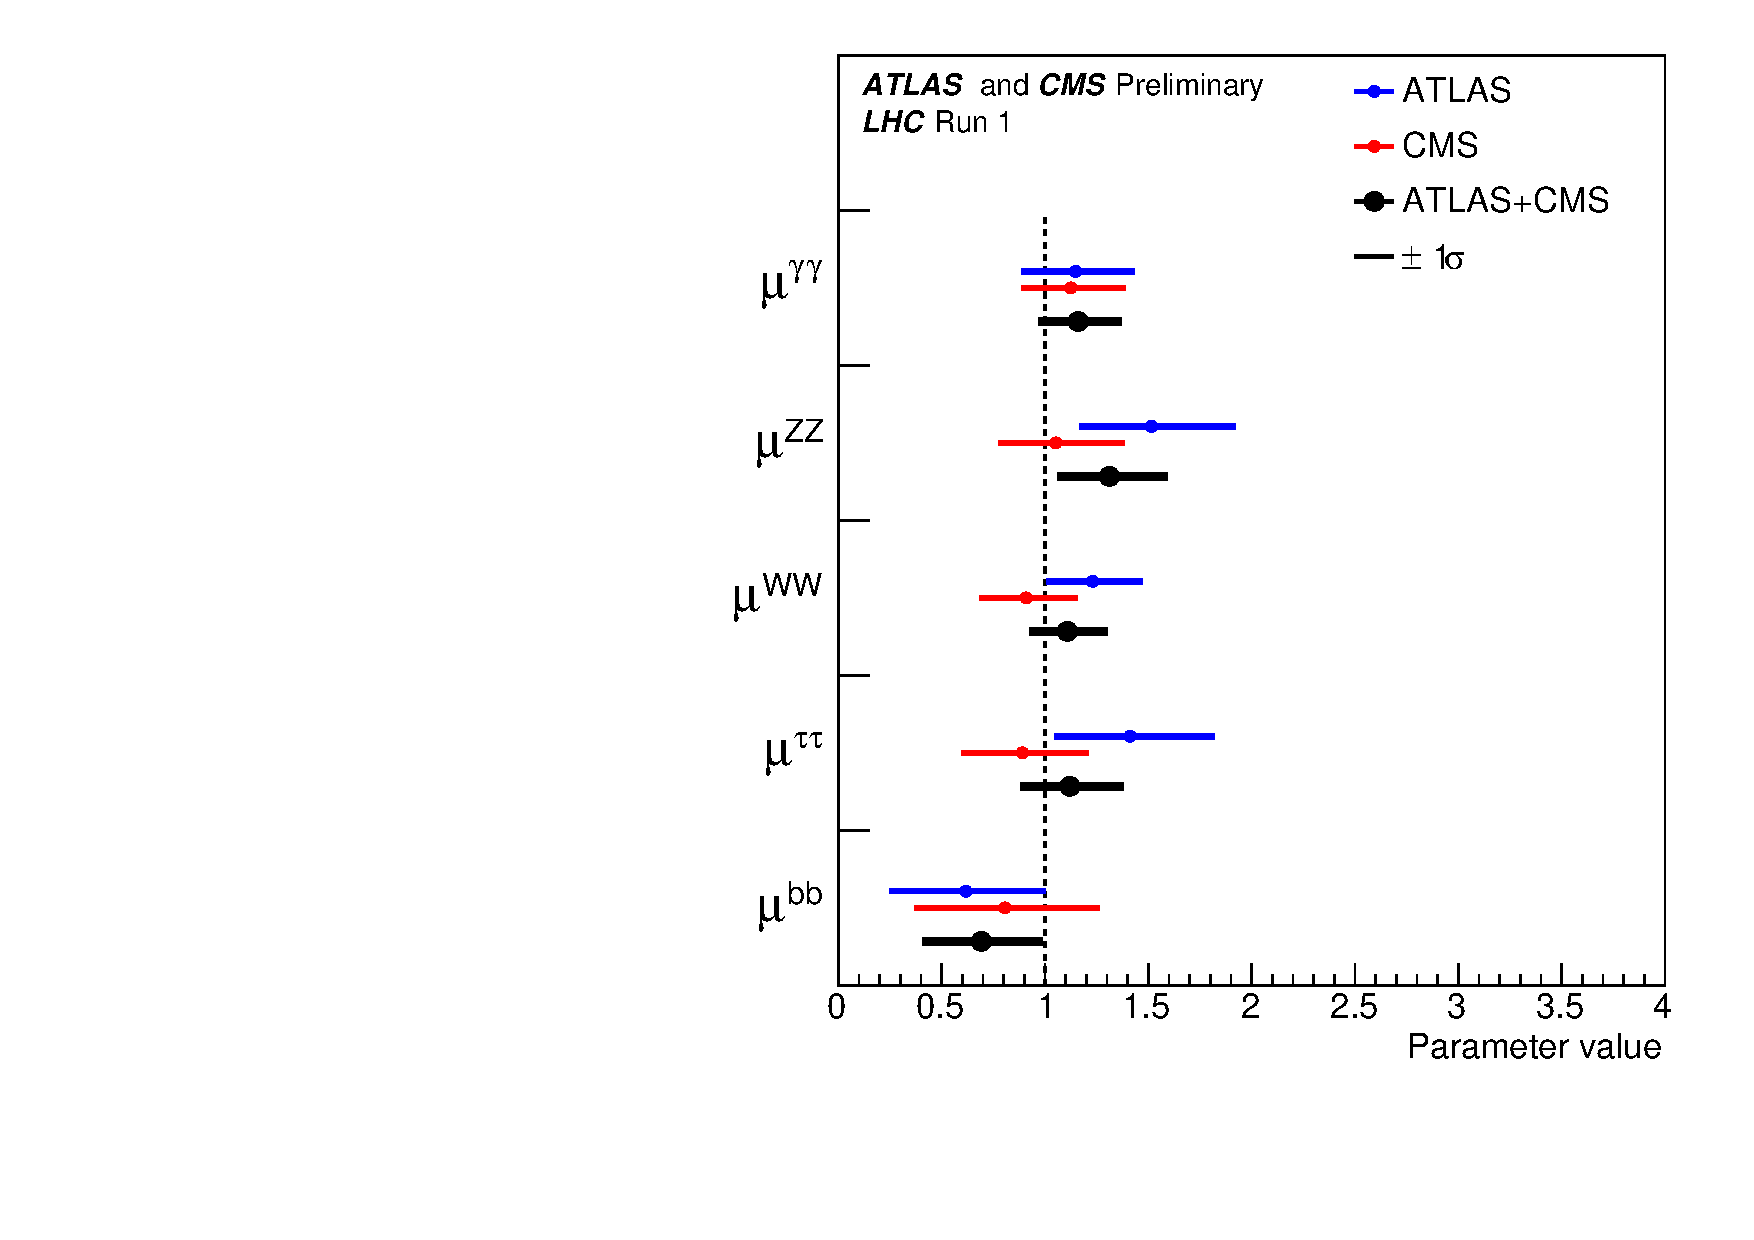
\includegraphics[width=.95\textwidth]{TalkPics/DM@LHC2016/CMS-PAS-HIG-15-002_Figure_012.pdf}
      \centering
      \scriptsize

      CMS-PAS-HIG-15-002
      
      ATLAS-CONF-2015-044
    \end{columns}
  \end{frame}

  \begin{frame}
    \frametitle{Why invisible particularly?}
    \begin{block}{}
      \begin{itemize}
      \item There is evidence from several sources for ``dark matter'' (DM)
      \item Where does dark matter get its mass from?
      \item Amounts of DM and SM matter seem to be of the same order of magnitude so it's likely they interact
      \end{itemize}
    \end{block}
    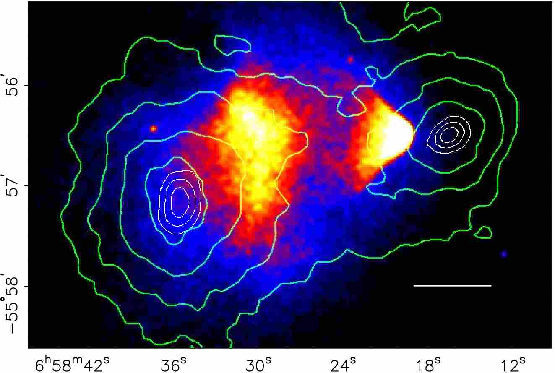
\includegraphics[clip=true,trim=0 0 0 0,height=.5\textheight,width=.5\textwidth]{TalkPics/sgs120315/bulletcluster.png}
    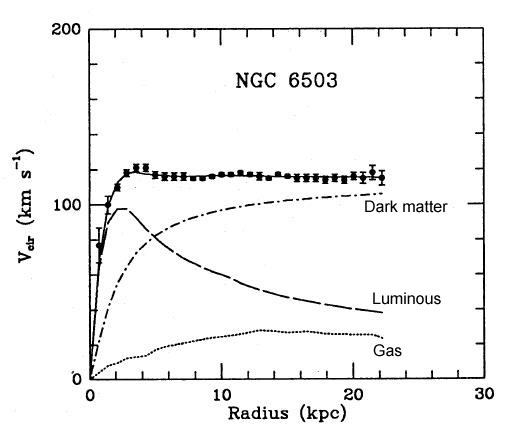
\includegraphics[clip=true,trim=0 0 0 0,height=.5\textheight,width=.5\textwidth]{TalkPics/sgs120315/rotationcurve.jpg}
  \end{frame}
  

  %Expand with mass term lagrangian and some DM intro
  \begin{frame}
    \frametitle{Why look for invisibly decaying Higgs bosons?}
    \vspace{-.3cm}
    \begin{columns}
      \column{1.06\textwidth}
    \begin{block}{}
      \small
      \begin{itemize}
      \item All massive SM particles get their mass through Higgs field couplings:
      \item[-] Fermions: $ \bar{\psi}_{i}y_{ij}\psi_{j}\phi+$ hermitian conjugate
      \item[-] Bosons: $|D_{\mu}\phi|^2-V(\phi)$
      \item Higgs mechanism is the only known locally gauge invariant way to give mass to particles charged under the SM symmetry groups
      \item DM must also get its mass from somewhere motivating interaction with a scalar like the Higgs
      \item Some theories of collider DM also have similar production mechanisms to the Higgs
      \end{itemize}
    \end{block}
    %feynman diagram of VBF
    \end{columns}
  \end{frame}
  

  %expand a bit more, decisions on fixed width etc.
  \begin{frame}
    \frametitle{How to search for invisibly decaying Higgs bosons}
    \vspace{-.2cm}
    \begin{columns}
      \column{.5\textwidth}
      \begin{block}{Indirect searches}
          \small
          \begin{itemize}
          \item Compare visible width to total width:
          \item[-] $\rm{BR}_{BSM}=\frac{\Gamma_{H}-\Gamma_{vis}}{\Gamma_{H}}$
          \item No measurement of $\Gamma_{H}$, need to make an assumption
          \item[-] Usually assume SM width
          \item ATLAS+CMS combination gives an observed (expected) limit on $\rm{BR}_{BSM}$ of 0.34 (0.35)
          \end{itemize}
      \end{block}
      \column{.5\textwidth}
      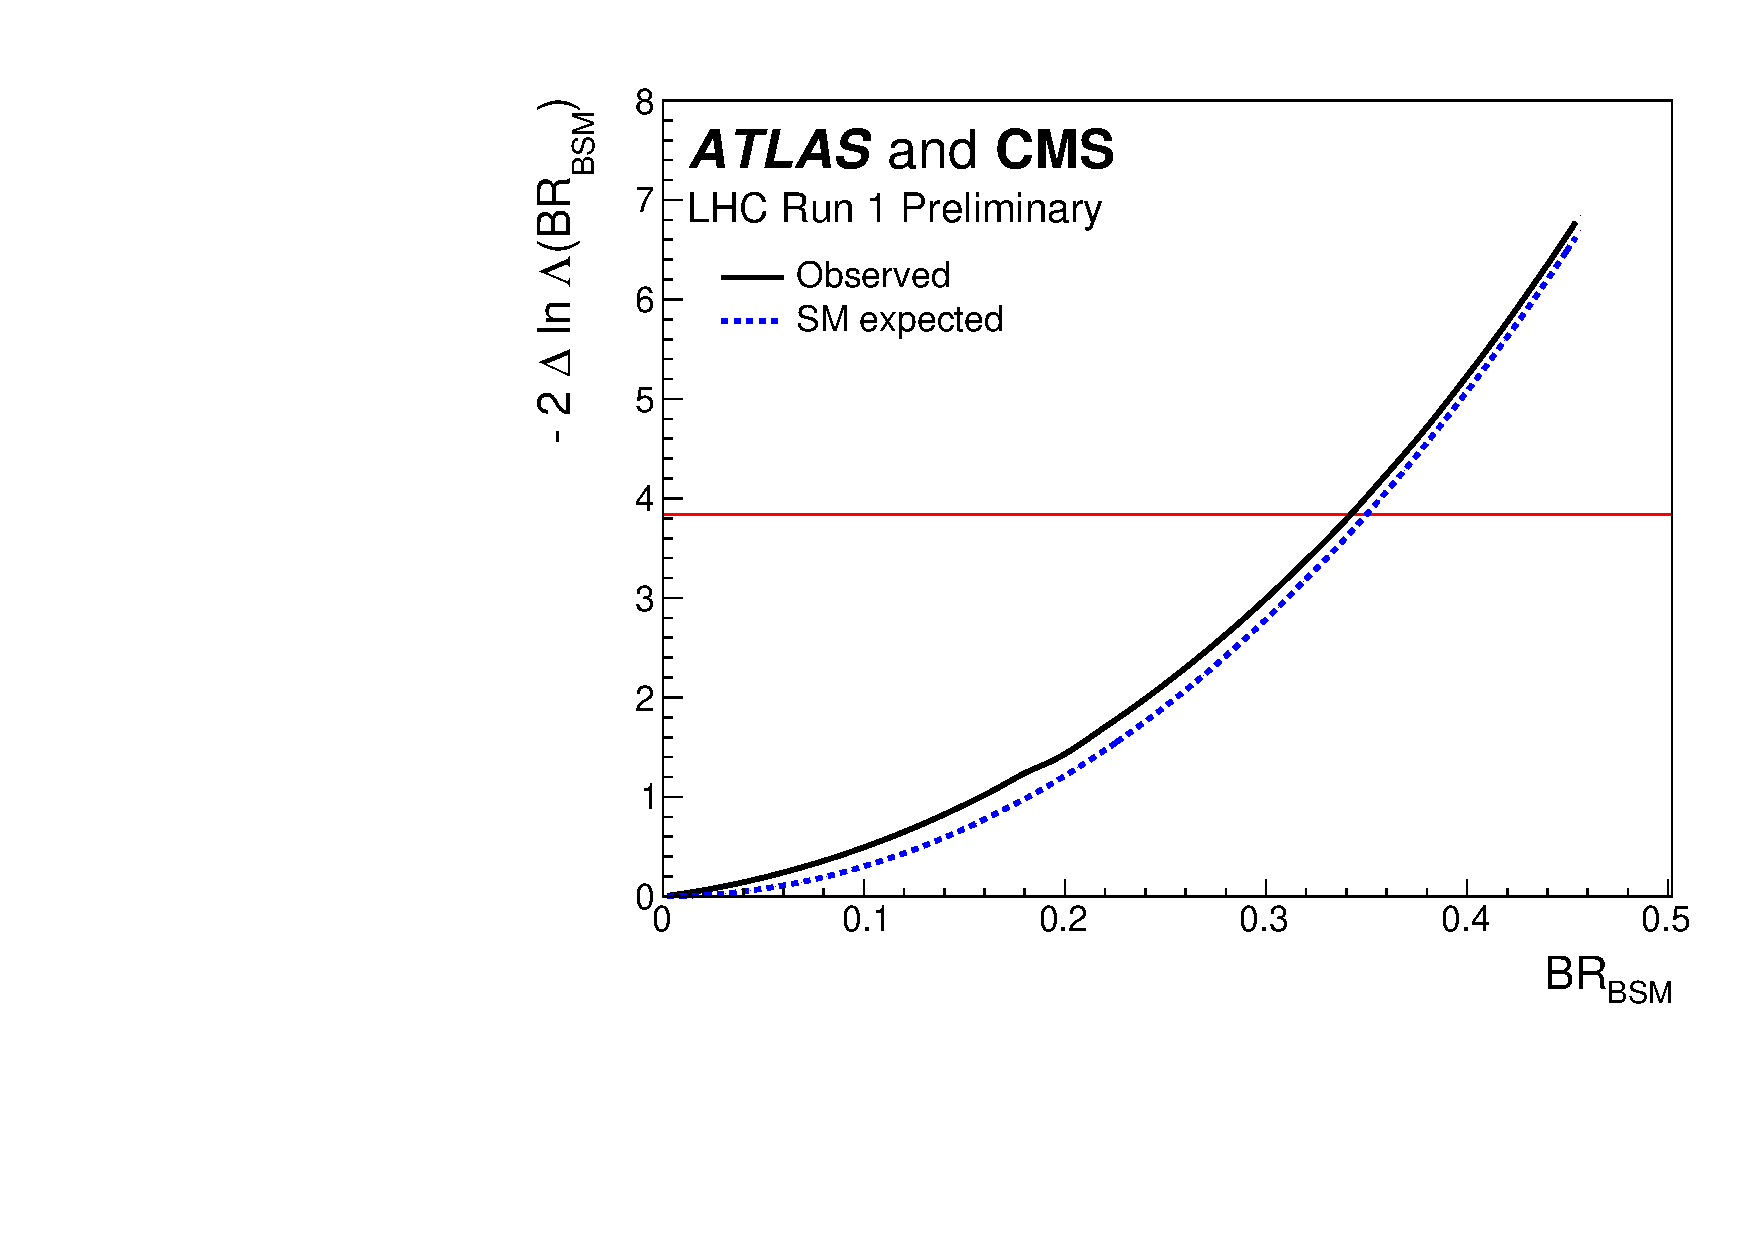
\includegraphics[width=\textwidth]{TalkPics/DM@LHC2016/CMS-PAS-HIG-15-002_Figure_015.pdf}
      \centering
      \scriptsize

      CMS-PAS-HIG-15-002
      
      ATLAS-CONF-2015-044
       \end{columns}
       %ATLAS or CMS rates of each channel plot
  \end{frame}

  %one slide on each process
  \begin{frame}
    \frametitle{How to search for invisibly decaying Higgs bosons}
    \begin{columns}
      \column{.5\textwidth}
      %diagram of MET
    \begin{block}{Direct searches}
      \begin{itemize}
      \item No visible products if Higgs boson is created alone
      \item Have to use associated Higgs production
      \item Tag associated production, then look for momentum imbalance ``$E_{T}^{miss}$''
      \end{itemize}
    \end{block}

      \column{.5\textwidth}
      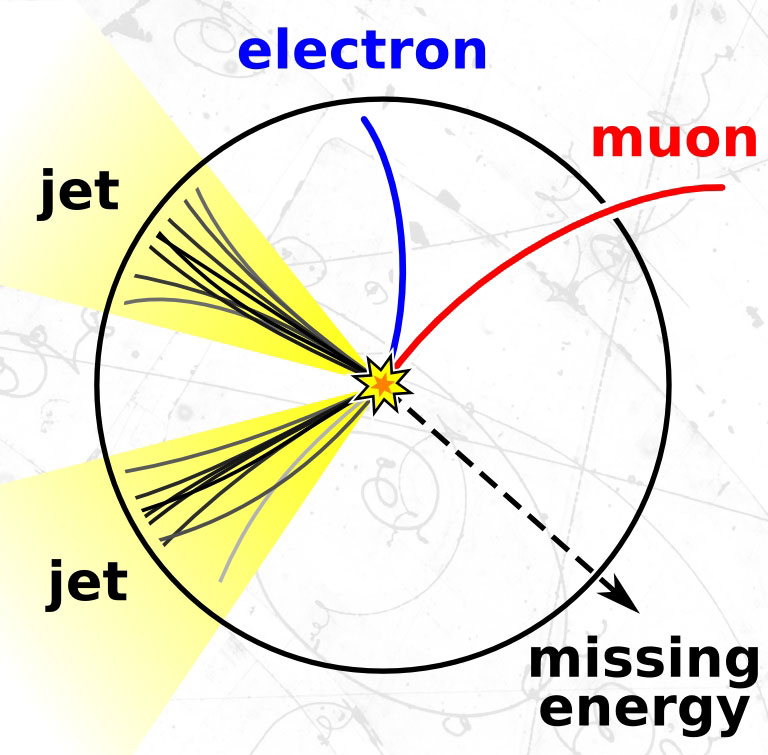
\includegraphics[width=\textwidth]{TalkPics/RHULSeminar051016/CMSResult042211figure1.jpg}
      \end{columns}
    \end{frame}

  %ggh
  \begin{frame}
    \frametitle{Gluon Fusion: ggH}
    \begin{columns}
      \column{.5\textwidth}
      \begin{block}{}
          \small
          %high rate low purity
          %ggH, VBF, VH tikz lines to plot if time
          \begin{itemize}
          \item Gluon fusion production has
            \tikz[na] \node (ggH) {\hspace{-.1cm} the highest rate \checkmark};
          \item Normally leaves no visible products $\boldsymbol{\times}$
          \item Only visible with initial state radiation (ISR)
          \item[-] ISR is difficult to tag and lowers rate
          \end{itemize}
      \end{block}
          
          \column{.5\textwidth}
            \centering
            \begin{fmfgraph*}(75,75)
              \fmfleft{i0,i2,ix,i3,i5}
              \fmfright{o0,o3,o1,o4,o6}
              \fmf{phantom,tension=4/3}{i2,v1,o3}
              \fmf{phantom,tension=4/3}{i3,v2,o4}
              \fmffreeze
              \fmf{gluon,tension=4/3}{i2,v1}
              \fmf{gluon,tension=4/3}{i3,v2}
              \fmf{fermion,tension=0}{v1,v2}
              \fmf{fermion,tension=2/3}{v2,v3,v1}
              \fmf{dashes}{v3,o1}
              \fmflabel{$g$}{i2}
              \fmflabel{$g$}{i3}
              \fmflabel{$H$}{o1}
            \end{fmfgraph*}

            \begin{tikzpicture}%[show background grid]
              \node [inner sep=0pt,above right]
                    {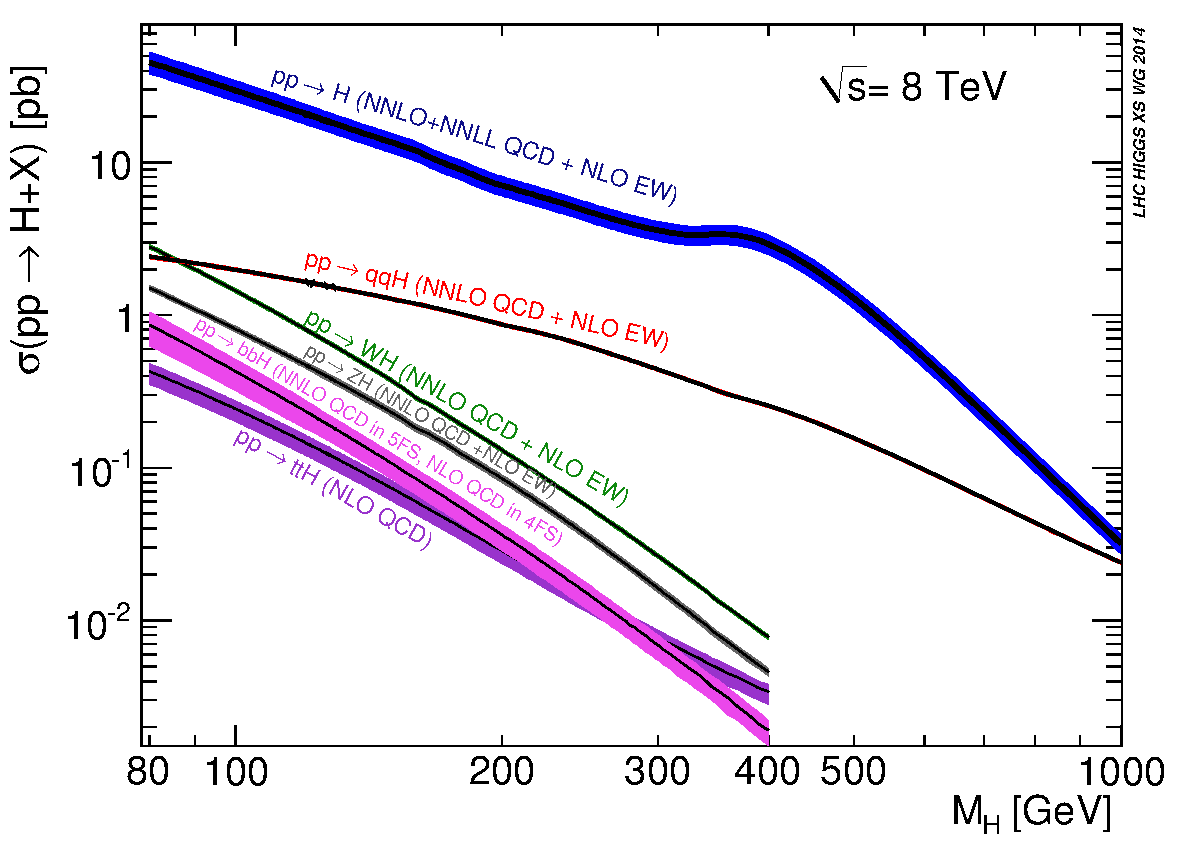
\includegraphics[width=\textwidth]{TalkPics/DM@LHC2016/XS_8TeV-eps-converted-to.pdf}};
                    %           \fill (0,0) circle (2pt);                                                                                                                                                                                                       
                    
                    \path (1.2,3.5) coordinate (ggHl)
                    (1.9,2.2) coordinate (VBFl)
                    (2.6,1.2) coordinate (ZHl);
            \end{tikzpicture}


            \begin{tikzpicture}[overlay]
              \path[->,blue,thick] (ggH.east) edge [bend left] (ggHl);
              %\path[->,red,thick] (VBF.west) edge [bend right] (VBFl);
              %\path[->,red,thick] (VBF.east) edge [bend left] (VBFdiag);
              %\path[->,green,thick] (ZH.south) edge [bend left] (ZHl);
              
            \end{tikzpicture}
            
      \end{columns}


  \end{frame}

  %zh
  \begin{frame}
    \frametitle{Vector boson associated production: VH}
    %high purity low rate
    \begin{columns}
      \column{.5\textwidth}
      \begin{block}{}
          \small
          %high rate low purity
          %ggH, VBF, VH tikz lines to plot if time
          \begin{itemize}
          \item VH production has a much
            \tikz[na] \node (VH) {\hspace{-.1cm}lower rate than ggH $\boldsymbol{\times}$};
          \item Leptonically decaying vector bosons are easy to tag \checkmark
          \item[-] Particularly $Z\rightarrow\ell\ell$ which was the first VH channel used
          \end{itemize}
      \end{block}
          
          \column{.5\textwidth}
            \centering
    \begin{fmfgraph*}(75,75)
      \fmfleft{i0,i1,i2,i3}
      \fmfright{o0,o1,o2,o3}
      \fmf{fermion}{i1,v1}
      \fmf{fermion}{v1,i2}
      \fmf{photon,label=$W,,Z$}{v1,v2}
      \fmf{photon}{v2,o1}
      \fmf{dashes}{v2,o2}
      \fmflabel{$q$}{i1}
      \fmflabel{$\bar{q}$}{i2}
      \fmflabel{$W,Z$}{o1}
      \fmflabel{$H$}{o2}
    \end{fmfgraph*}
            
            \begin{tikzpicture}%[show background grid]
              \node [inner sep=0pt,above right]
                    {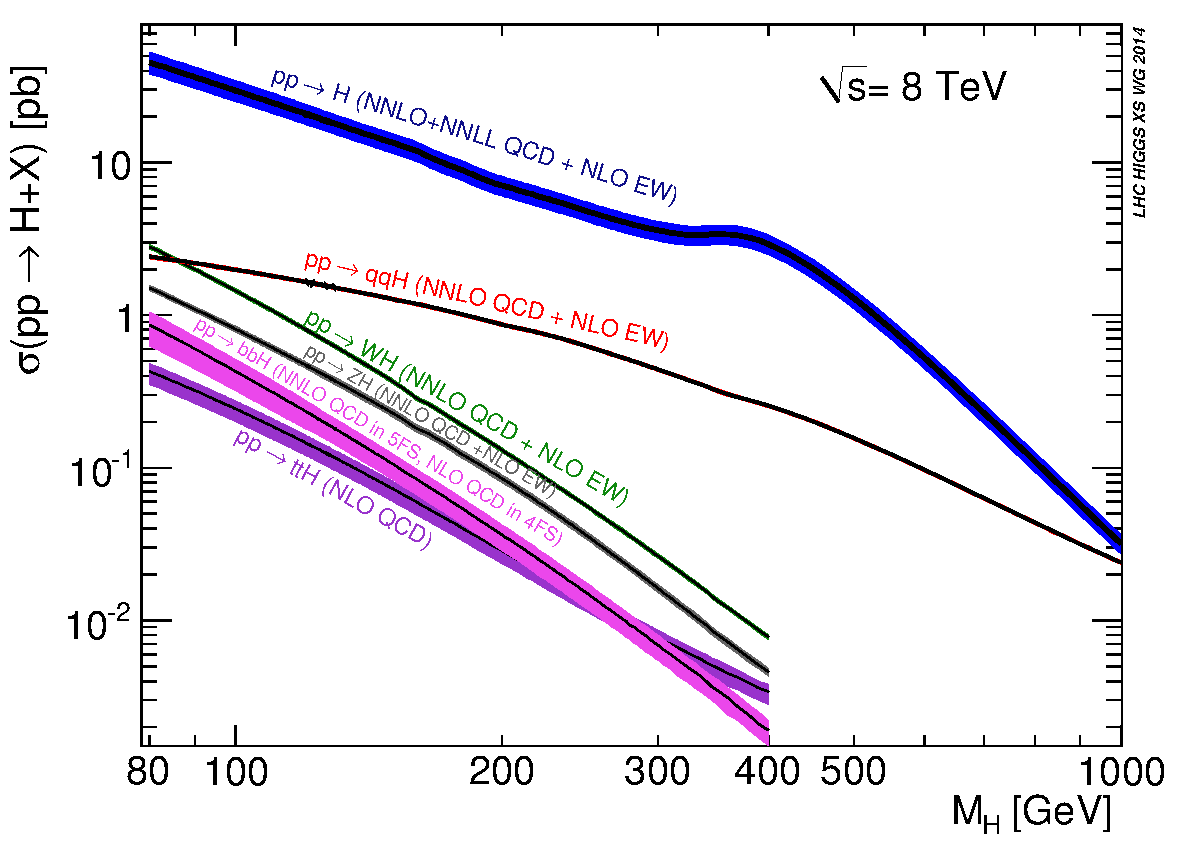
\includegraphics[width=\textwidth]{TalkPics/DM@LHC2016/XS_8TeV-eps-converted-to.pdf}};
                    %           \fill (0,0) circle (2pt);                                                                                                                                                                                                       
                    
                    \path (1.2,3.5) coordinate (ggHl)
                    (1.9,2.2) coordinate (VBFl)
                    (2.6,1.5) coordinate (ZHl);
            \end{tikzpicture}


            \begin{tikzpicture}[overlay]
              %\path[->,blue,thick] (ggH.east) edge [bend left] (ggHl);
              %\path[->,red,thick] (VBF.west) edge [bend right] (VBFl);
              %\path[->,red,thick] (VBF.east) edge [bend left] (VBFdiag);
              \path[->,green,thick] (VH.east) edge [bend left] (ZHl);
              
            \end{tikzpicture}
            
      \end{columns}

  \end{frame}

  %vbf
  \begin{frame}
    \frametitle{Vector Boson Fusion: VBF}
    %best of both worlds
    \begin{columns}
      \column{.5\textwidth}
      \begin{block}{}
          \small
          %high rate low purity
          %ggH, VBF, VH tikz lines to plot if time
          \begin{itemize}
          \item VBF has a relatively high
            \tikz[na] \node (VBF) {\hspace{-.1cm}production rate \checkmark};
          \item Lack of strong force `colour connection' leaves large polar angle between quarks
          \item[-] This allows the resulting jets to be tagged \checkmark
          \item Focus of the rest of the talk
          \end{itemize}
      \end{block}
          
          \column{.5\textwidth}
            \centering
            \begin{fmfgraph*}(75,75)
              \fmfleft{i0,i1,i2,i3}
              \fmfright{o0,o1,o2,o3,o4}
              \fmf{fermion}{i1,v1,o1}
              \fmf{fermion}{i2,v2,o3}
              \fmf{photon}{v1,v3}
              \fmf{photon,label=$W,,Z$}{v2,v3}
              \fmf{dashes}{v3,o2}
              \fmflabel{$q$}{i1}
              \fmflabel{$q$}{i2}
              \fmflabel{$q$}{o1}
              \fmflabel{$q$}{o3}
              \fmflabel{$H$}{o2}
            \end{fmfgraph*}

            \begin{tikzpicture}%[show background grid]
              \node [inner sep=0pt,above right]
                    {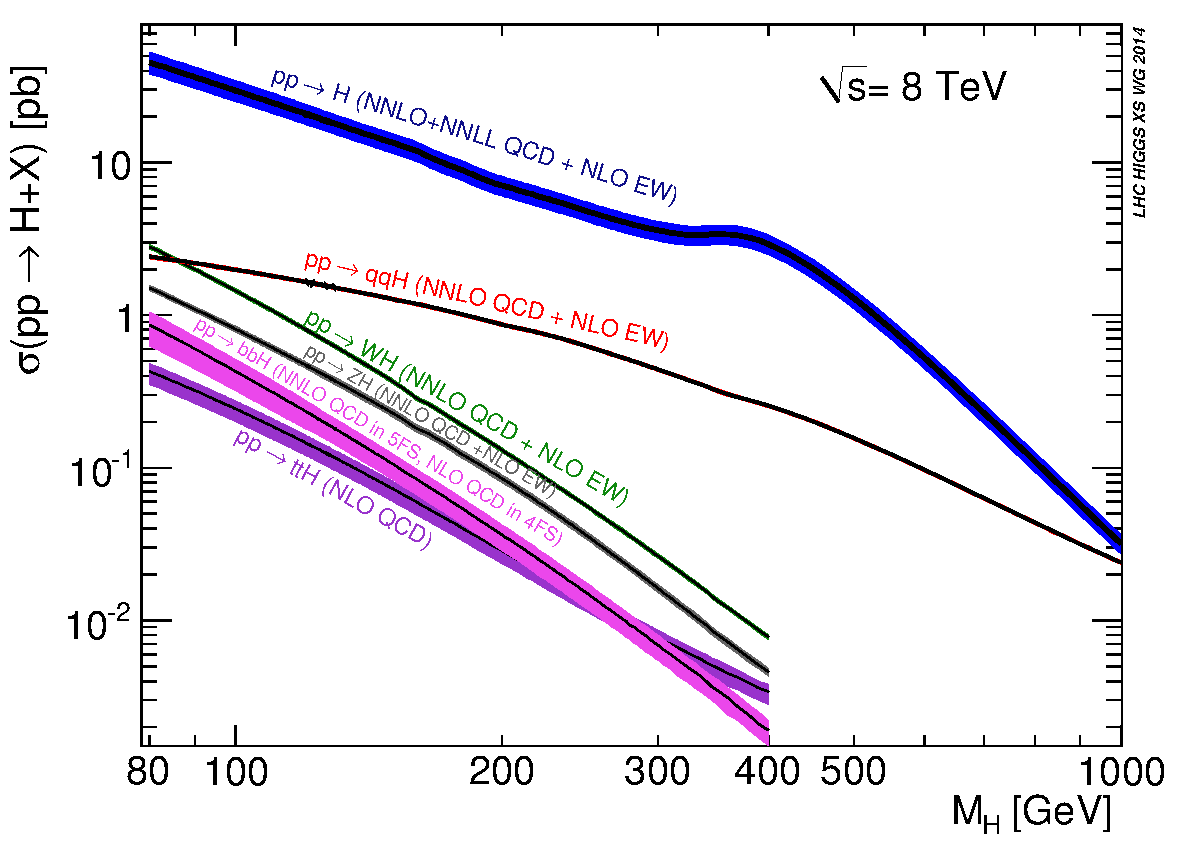
\includegraphics[width=\textwidth]{TalkPics/DM@LHC2016/XS_8TeV-eps-converted-to.pdf}};
                    %           \fill (0,0) circle (2pt);                                                                                                                                                                                                       
                    
                    \path (1.2,3.5) coordinate (ggHl)
                    (1.9,2.6) coordinate (VBFl)
                    (2.6,1.2) coordinate (ZHl);
            \end{tikzpicture}


            \begin{tikzpicture}[overlay]
              %\path[->,blue,thick] (ggH.east) edge [bend left] (ggHl);
              \path[->,red,thick] (VBF.east) edge [bend left] (VBFl);
              %\path[->,red,thick] (VBF.east) edge [bend left] (VBFdiag);
              %\path[->,green,thick] (ZH.south) edge [bend left] (ZHl);
              
            \end{tikzpicture}
            
      \end{columns}

  \end{frame}

  %ttH
  \begin{frame}
    \frametitle{ttH}
    %aside just for completeness
    \begin{columns}
      \column{.5\textwidth}
      \begin{block}{}
          \small
          \begin{itemize}
          \item \tikz[na] \node (ttH) {ttH has a very low rate $\boldsymbol{\times}$$\boldsymbol{\times}$};
          \item Taggable decay products \checkmark
          \item Not sensitive with LHC Run 1 data
          \item[-] Starting to become interesting with higher Run 2 energy
          \end{itemize}
      \end{block}
          
          \column{.5\textwidth}
            \centering
            \vspace{.5cm}
            \begin{fmfgraph*}(75,50)
              \fmfleft{i1,i2}
              \fmfright{o1,o2,o3}
              \fmf{gluon}{i1,v1}
              \fmf{gluon}{i2,v2}
              \fmf{fermion}{o1,v1,v3,v2,o3}
              \fmf{dashes}{v3,o2}
              \fmflabel{$t$}{o1}
              \fmflabel{$t$}{o3}
              \fmflabel{$H$}{o2}
            \end{fmfgraph*}
            \vspace{.2cm}
            \begin{tikzpicture}%[show background grid]
              \node [inner sep=0pt,above right]
                    {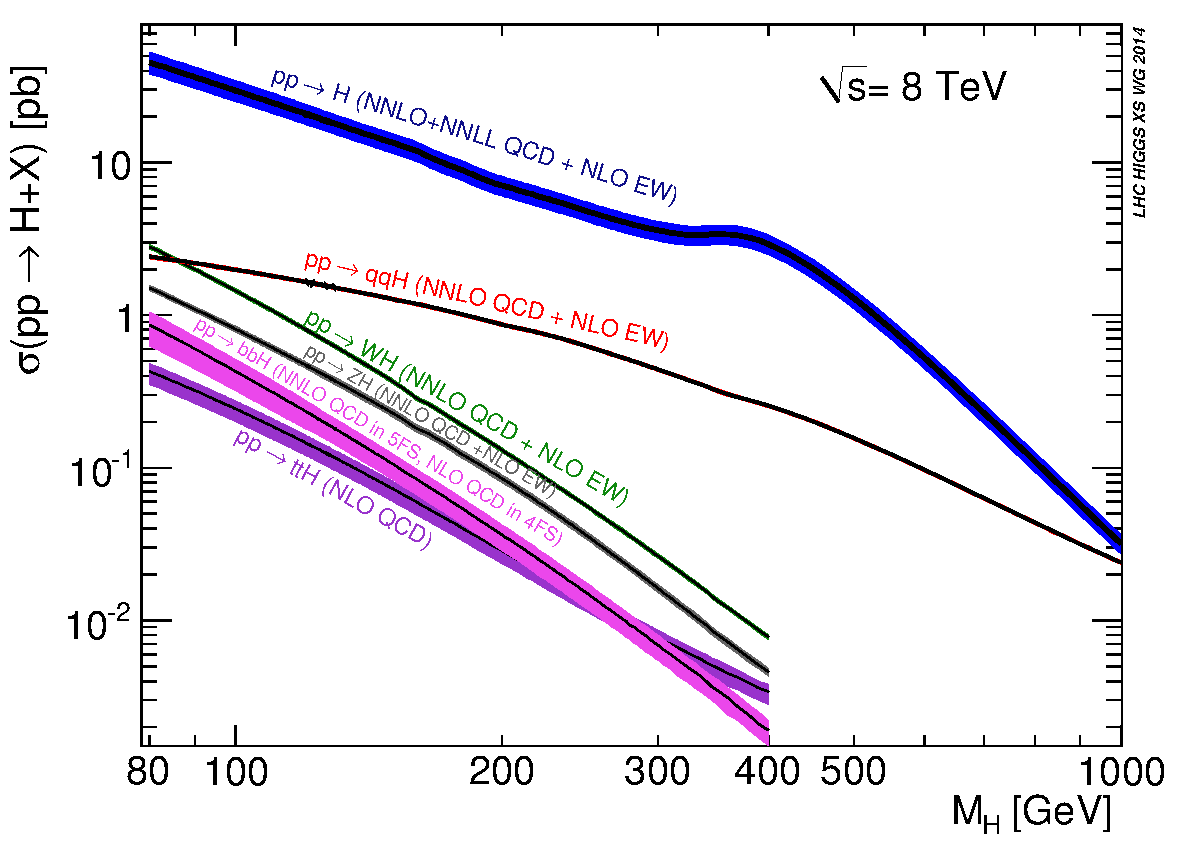
\includegraphics[width=\textwidth]{TalkPics/DM@LHC2016/XS_8TeV-eps-converted-to.pdf}};
                    %           \fill (0,0) circle (2pt);                                                                                                                                                                                                       
                    
                    \path (1.2,3.5) coordinate (ggHl)
                    (1.9,2.2) coordinate (VBFl)
                    (2.6,1.2) coordinate (ZHl)
                    (2.6,1.2) coordinate (ttHl);
            \end{tikzpicture}


            \begin{tikzpicture}[overlay]
              \path[->,violet,thick] (ttH.east) edge [bend left] (ttHl);
              %\path[->,red,thick] (VBF.west) edge [bend right] (VBFl);
              %\path[->,red,thick] (VBF.east) edge [bend left] (VBFdiag);
              %\path[->,green,thick] (ZH.south) edge [bend left] (ZHl);
              
            \end{tikzpicture}
            
      \end{columns}

  \end{frame}


  %why CMS is good for invisible detection
  \begin{frame}
    \frametitle{What detector capabilities do we need?}
    %things needed to see VBF i.e. jets and met
    \begin{block}{}
      \begin{itemize}
      \item VBF jets have a large polar angle separation
      \item[-] Calorimetry close to the beamline is important
      \item $E_{T}^{miss}$ measurement accuracy requires a 4$\pi$ hermitic detector
      \item Good energy resolution for all objects is also necessary
      \end{itemize}
    \end{block}
    \vspace{.4cm}
            \centering
            \begin{fmfgraph*}(75,75)
              \fmfleft{i1,i2}
              \fmfright{o1,o2,o3}
              \fmf{fermion}{i1,v1,o1}
              \fmf{fermion}{i2,v2,o3}
              \fmf{photon,label=$W,,Z$}{v1,v3}
              \fmf{photon,label=$W,,Z$}{v2,v3}
              \fmf{dashes}{v3,o2}
              \fmflabel{$q$}{i1}
              \fmflabel{$q$}{i2}
              \fmflabel{$q$}{o1}
              \fmflabel{$q$}{o3}
              \fmflabel{$H$}{o2}
            \end{fmfgraph*}

  \end{frame}

  \begin{frame}
    \frametitle{CMS}
    \begin{block}{}
      \begin{itemize}
      \item Detector covers pseudorapidities up to 5
      \end{itemize}
    \end{block}
    \centering
    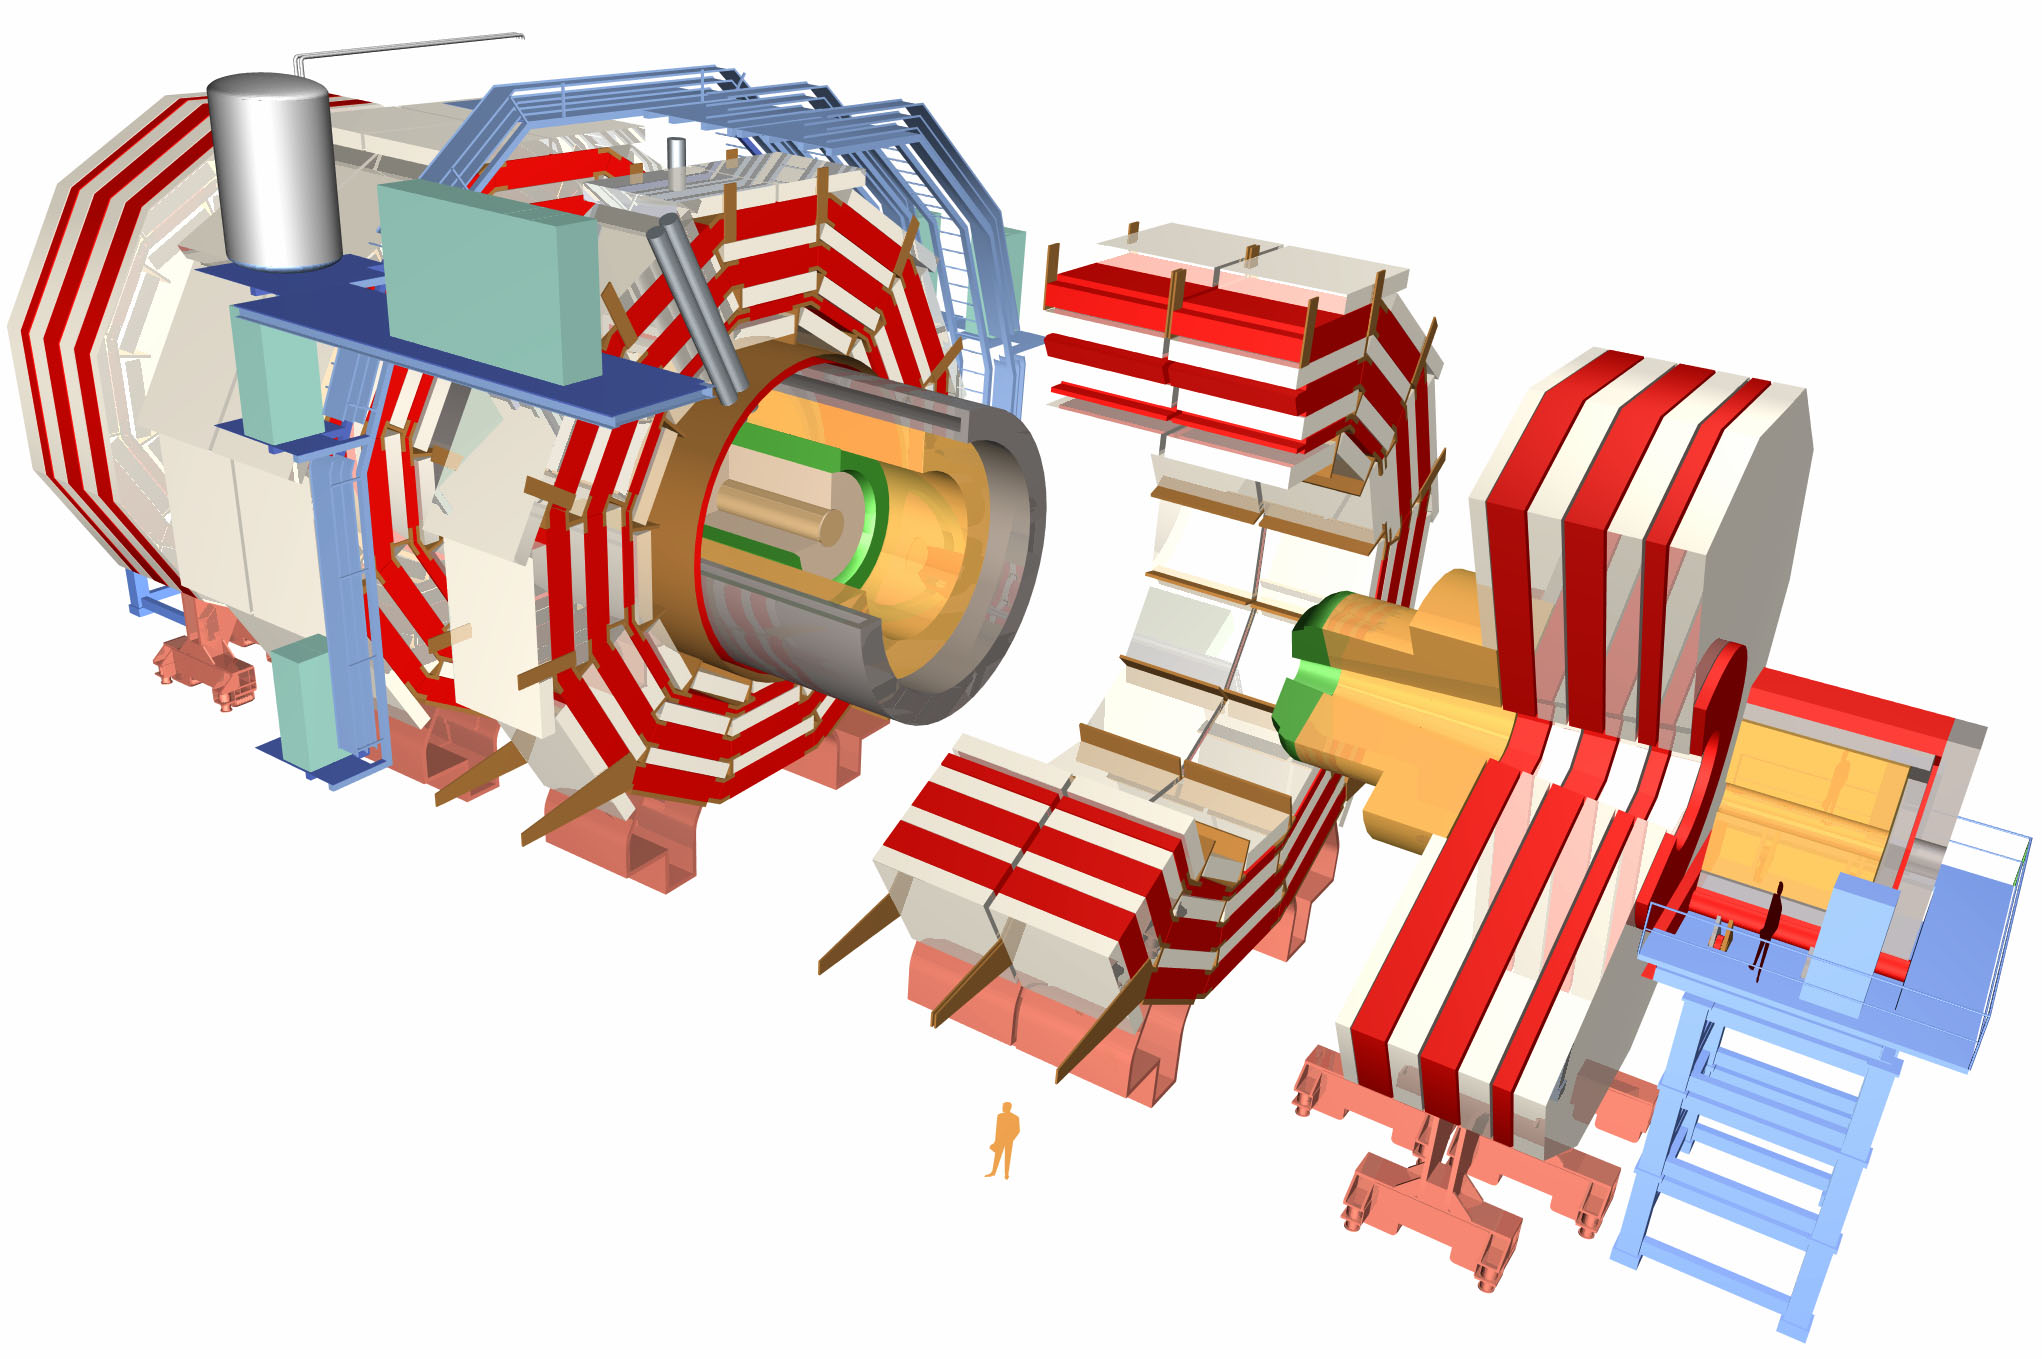
\includegraphics[width=.9\textwidth]{TalkPics/RHULSeminar051016/detector.jpg}
  \end{frame}

  %bit on particle flow
  \begin{frame}
    \frametitle{CMS particle flow reconstruction}
    \begin{columns}
      \column{1.06\textwidth}
      \vspace{-.3cm}
      \begin{block}{}
        \scriptsize
        \begin{itemize}
        \item 4T magnet and tracking system give good momentum measurements
        \item PbWO$_{4}$ crystal ECAL gives good EM energy resolution
        \item CMS HCAL is the least precise subdetector
        \item[-] What about jet energy resolution?
        \end{itemize}
      \end{block}
    \end{columns}
    \centering
    \vspace{.1cm}
    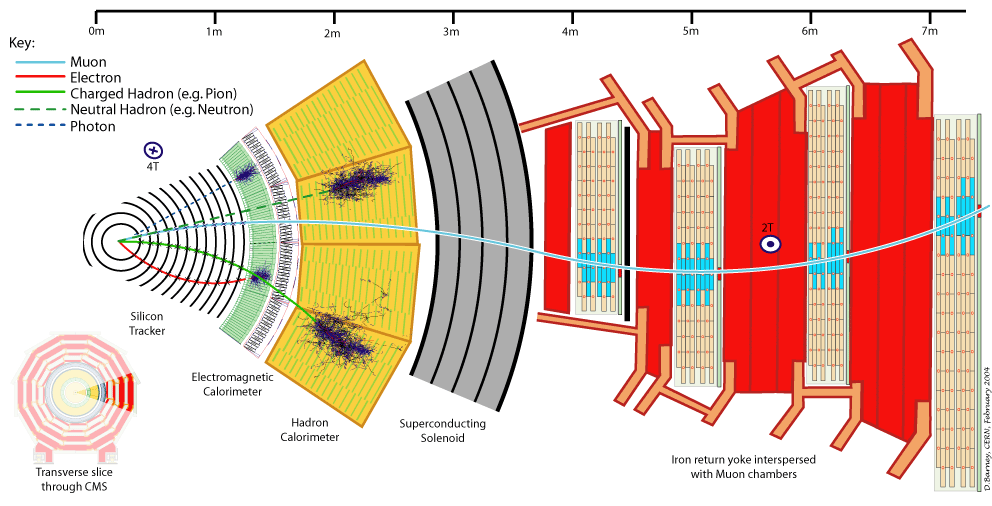
\includegraphics[width=.9\textwidth]{TalkPics/CMS_Slice.png}
  \end{frame}

  %bit on met and jet corrections
  \begin{frame}
    \frametitle{Particle flow}
    \begin{columns}
      \column{.6\textwidth}
      \begin{block}{}
        \begin{itemize}
        \item Particle flow links information from all subdetectors
        \item Jets mostly consist of charged hadrons (60\%) and $e/\gamma$ (30\%)
        \item[-] Charged hadron deposits in HCAL can be matched to precise tracker measurements
        \item[-] $e/\gamma$ can be measured in the ECAL
        \item This leaves only 10\% of the jet measured by the HCAL
        \item Good resolution of all objects allows accurate $E_{T}^{miss}$ calculation
        \end{itemize}
      \end{block}
      \column{.4\textwidth}
      Jets
      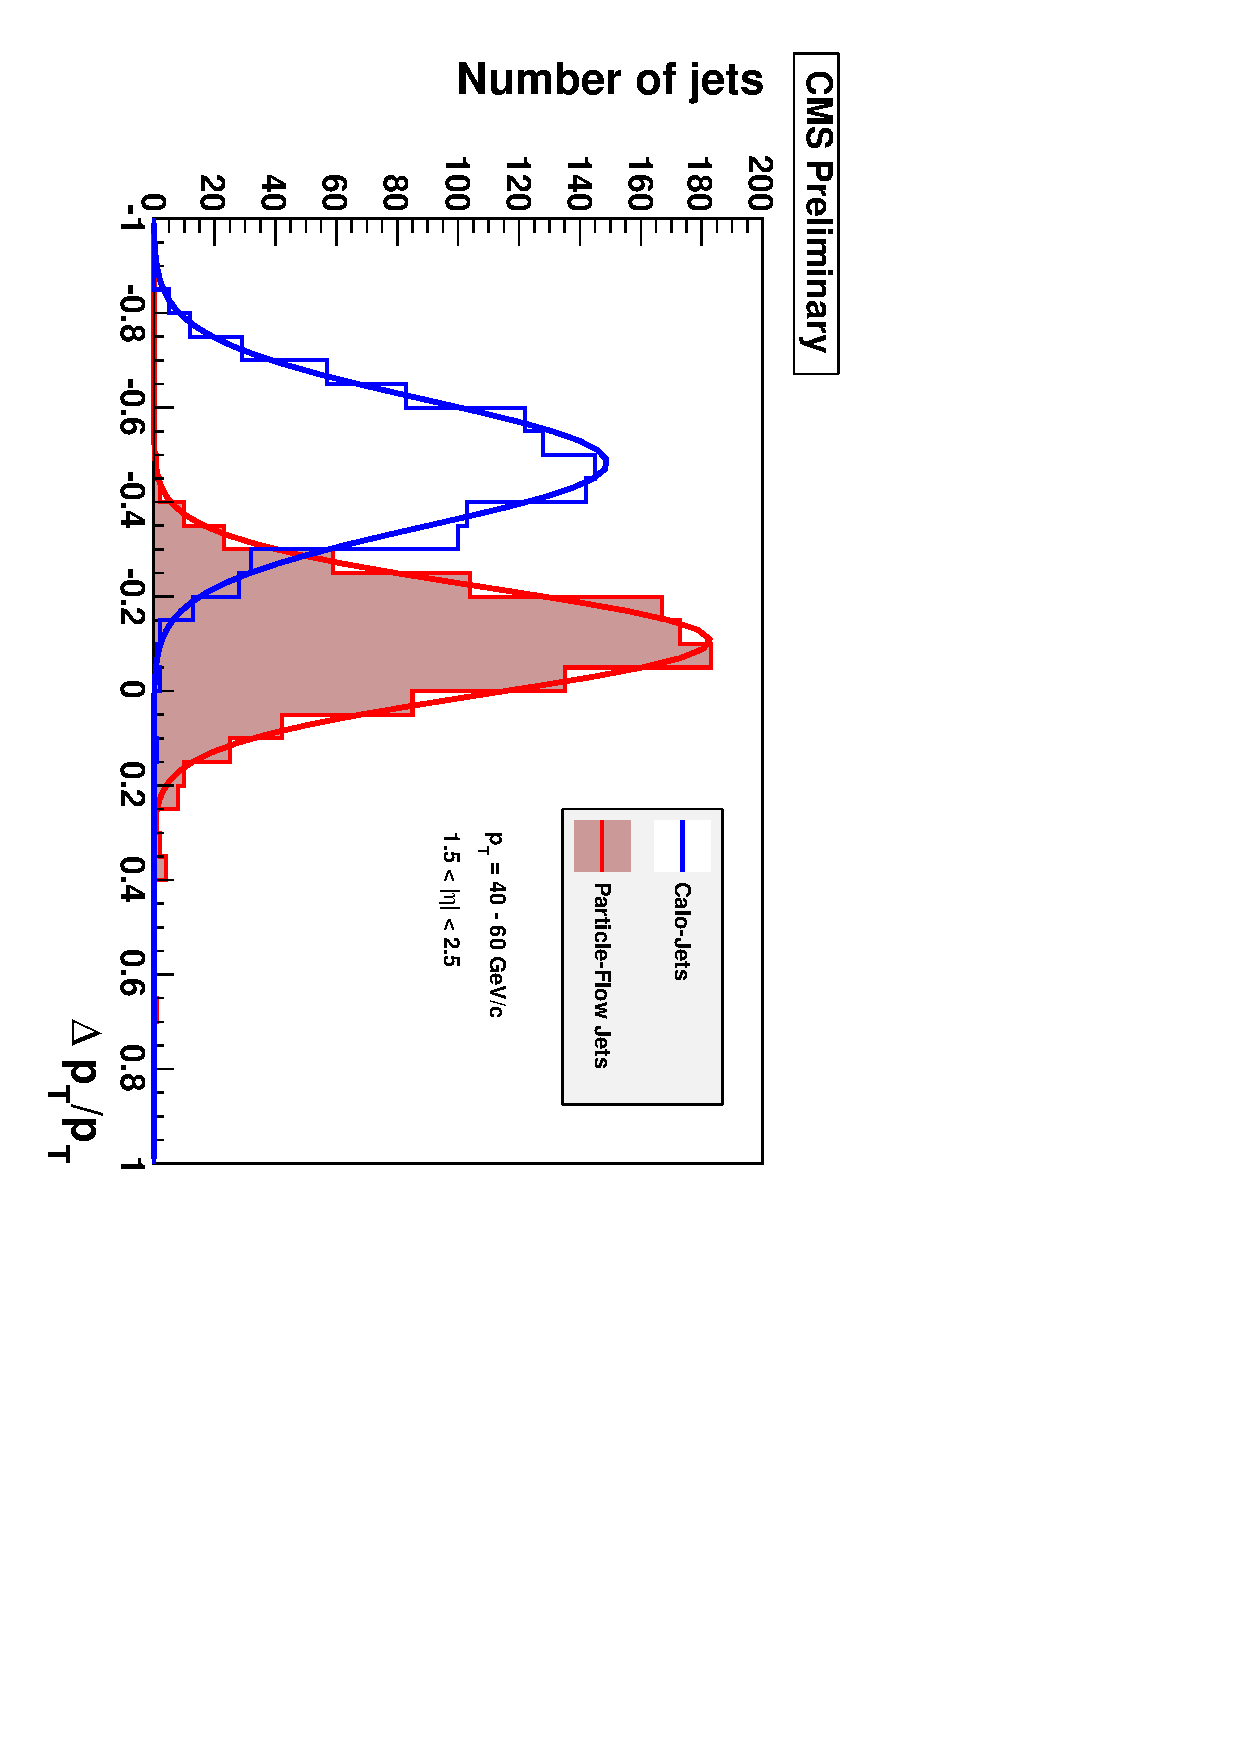
\includegraphics[angle=90,width=\textwidth]{TalkPics/RHULSeminar051016/particleflow.pdf}
      
      $E_{T}^{miss}$
      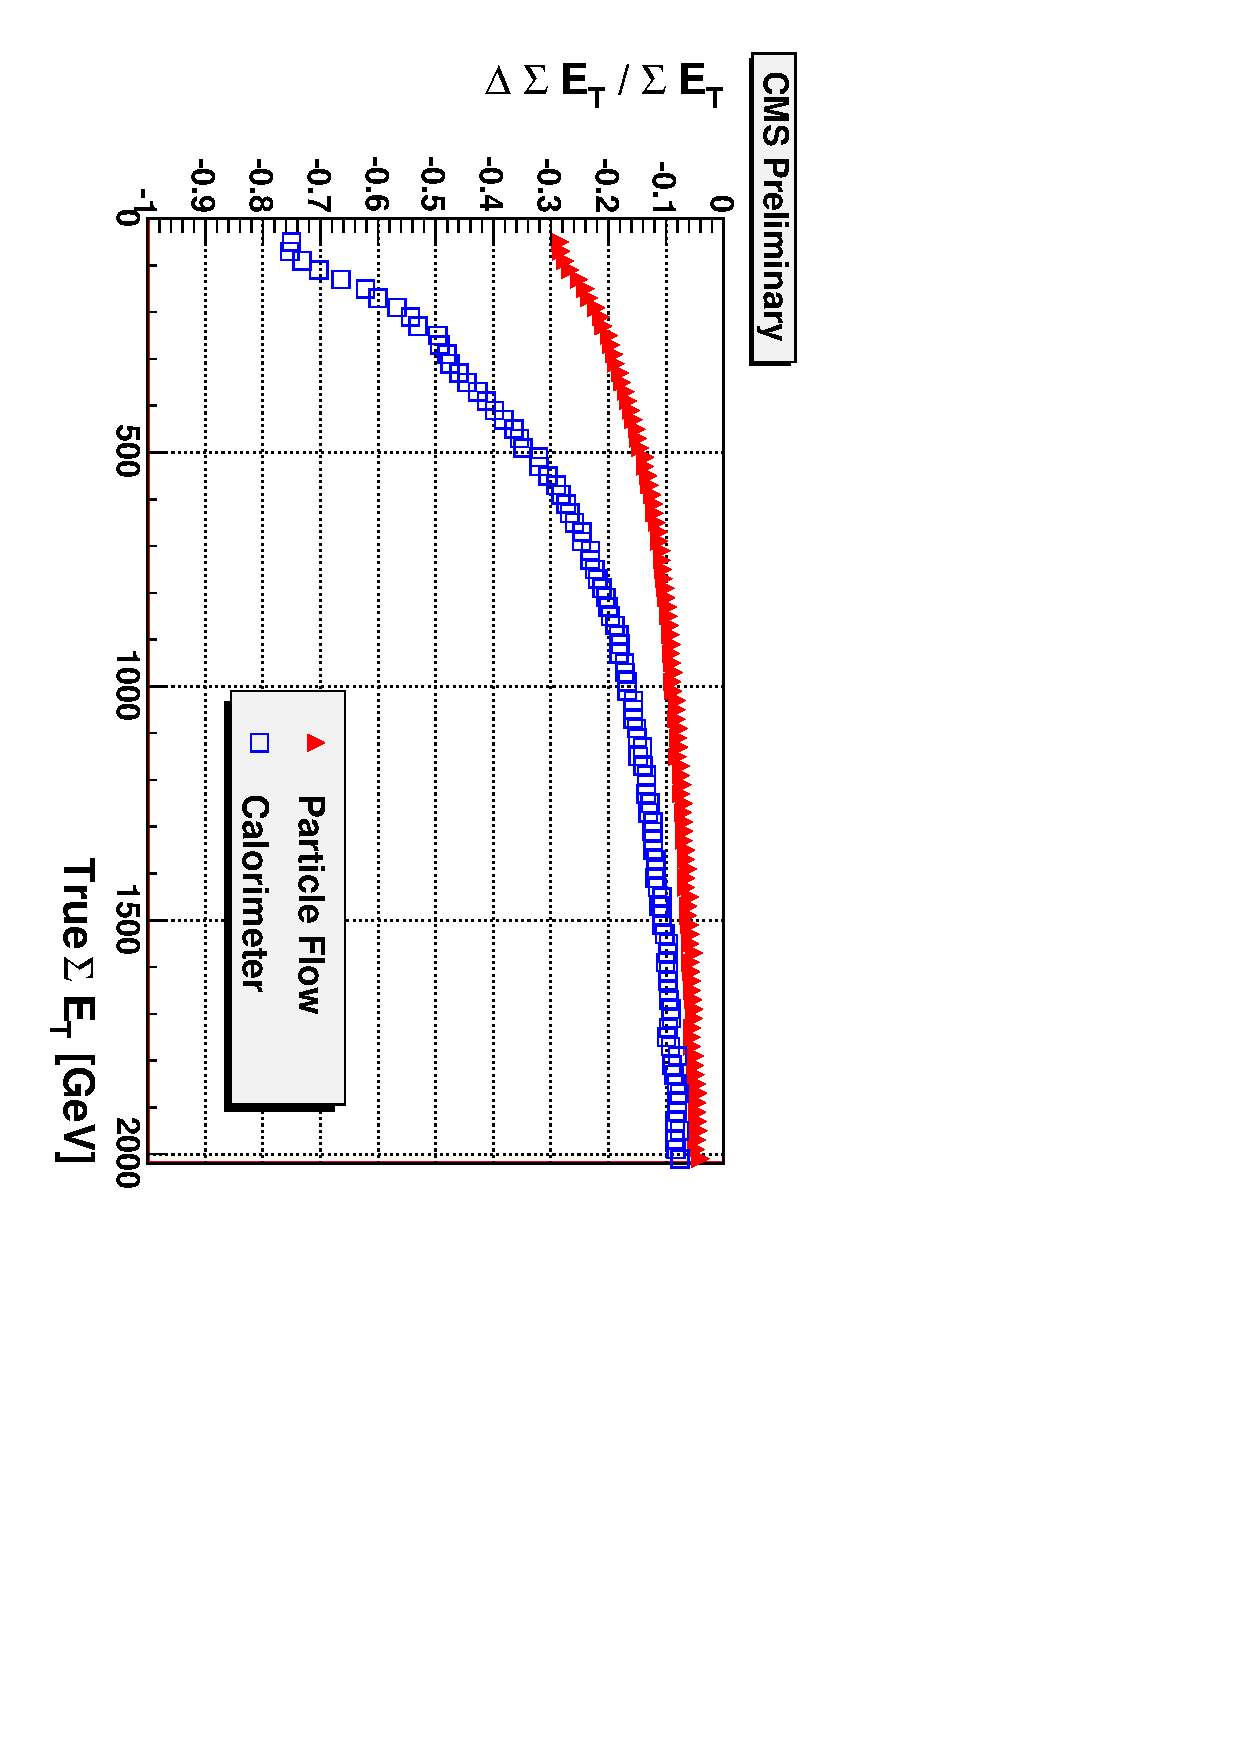
\includegraphics[angle=90,width=\textwidth]{TalkPics/RHULSeminar051016/particleflowmet.pdf}
    \end{columns}
  \end{frame}

  %Outline challenges of VBF analysis trigger/high QCD background
  \begin{frame}
    \frametitle{Main challenges for VBF Higgs to invisible}
    \begin{columns}
      \column{.5\textwidth}
      \begin{block}{}
        \begin{itemize}
        \item QCD multijet production cross-section is much larger than signal cross-section
        \item[-] Some of these jets will fake the VBF topology
        \item Trigger must be very tight to reduce event rate to an acceptable level
        \item Significant remaining QCD background is hard to model
        \end{itemize}
      \end{block}
      \column{.5\textwidth}
      \centering
      Signal

      \vspace{.5cm}

      \begin{fmfgraph*}(45,60)
        \fmftop{i1,m1,m2,m3,m4,o1}
        \fmfbottom{i2,o2}
        \fmf{fermion,tension=4}{v1,i2}
        \fmf{fermion,tension=4}{v1,o2}
        \fmf{phantom}{v1,m1}
        \fmf{dashes}{v1,m2}
        \fmf{phantom}{v1,m3}
        \fmf{phantom}{v1,m4}
        \fmflabel{$H$}{m2}
        \fmflabel{$jet$}{i2}
        \fmflabel{$jet$}{o2}
      \end{fmfgraph*}

      \vspace{.5cm}

      QCD background

      \begin{fmfgraph*}(45,60)
        \fmftop{i1,m1,m2,m3,m4,o1}
        \fmfbottom{i2,o2}
        \fmf{fermion,tension=4}{v1,i2}
        \fmf{fermion,tension=4}{v1,o2}
        \fmf{fermion,label=$jets$,label.side=left}{v1,m1}
        \fmf{fermion}{v1,m2}
        \fmf{fermion}{v1,m3}
        \fmf{fermion}{v1,m4}
        \fmflabel{$jet$}{i2}
        \fmflabel{$jet$}{o2}
      \end{fmfgraph*}
    \end{columns}
  \end{frame}

  %parked data
  \begin{frame}
    \frametitle{Parked data}
    \begin{block}{}
      \scriptsize
      \begin{itemize}
      \item Limiting factor in CMS event rate found to be processing time, not data output
      \item During Run 1 about a third of data was 'promptly' reconstructed
      \item[-] Remaining two thirds were 'parked' for reconstruction in the long shutdown
      \item This parked data has much looser trigger thresholds
      \item Dedicated VBF invisible Higgs triggers were run for both streams
      \end{itemize}
    \end{block}
    \vspace{-.05cm}
    \centering
    \begin{columns}
      \column{1.1\textwidth}
      \begin{tikzpicture}
          \node (l1node){
            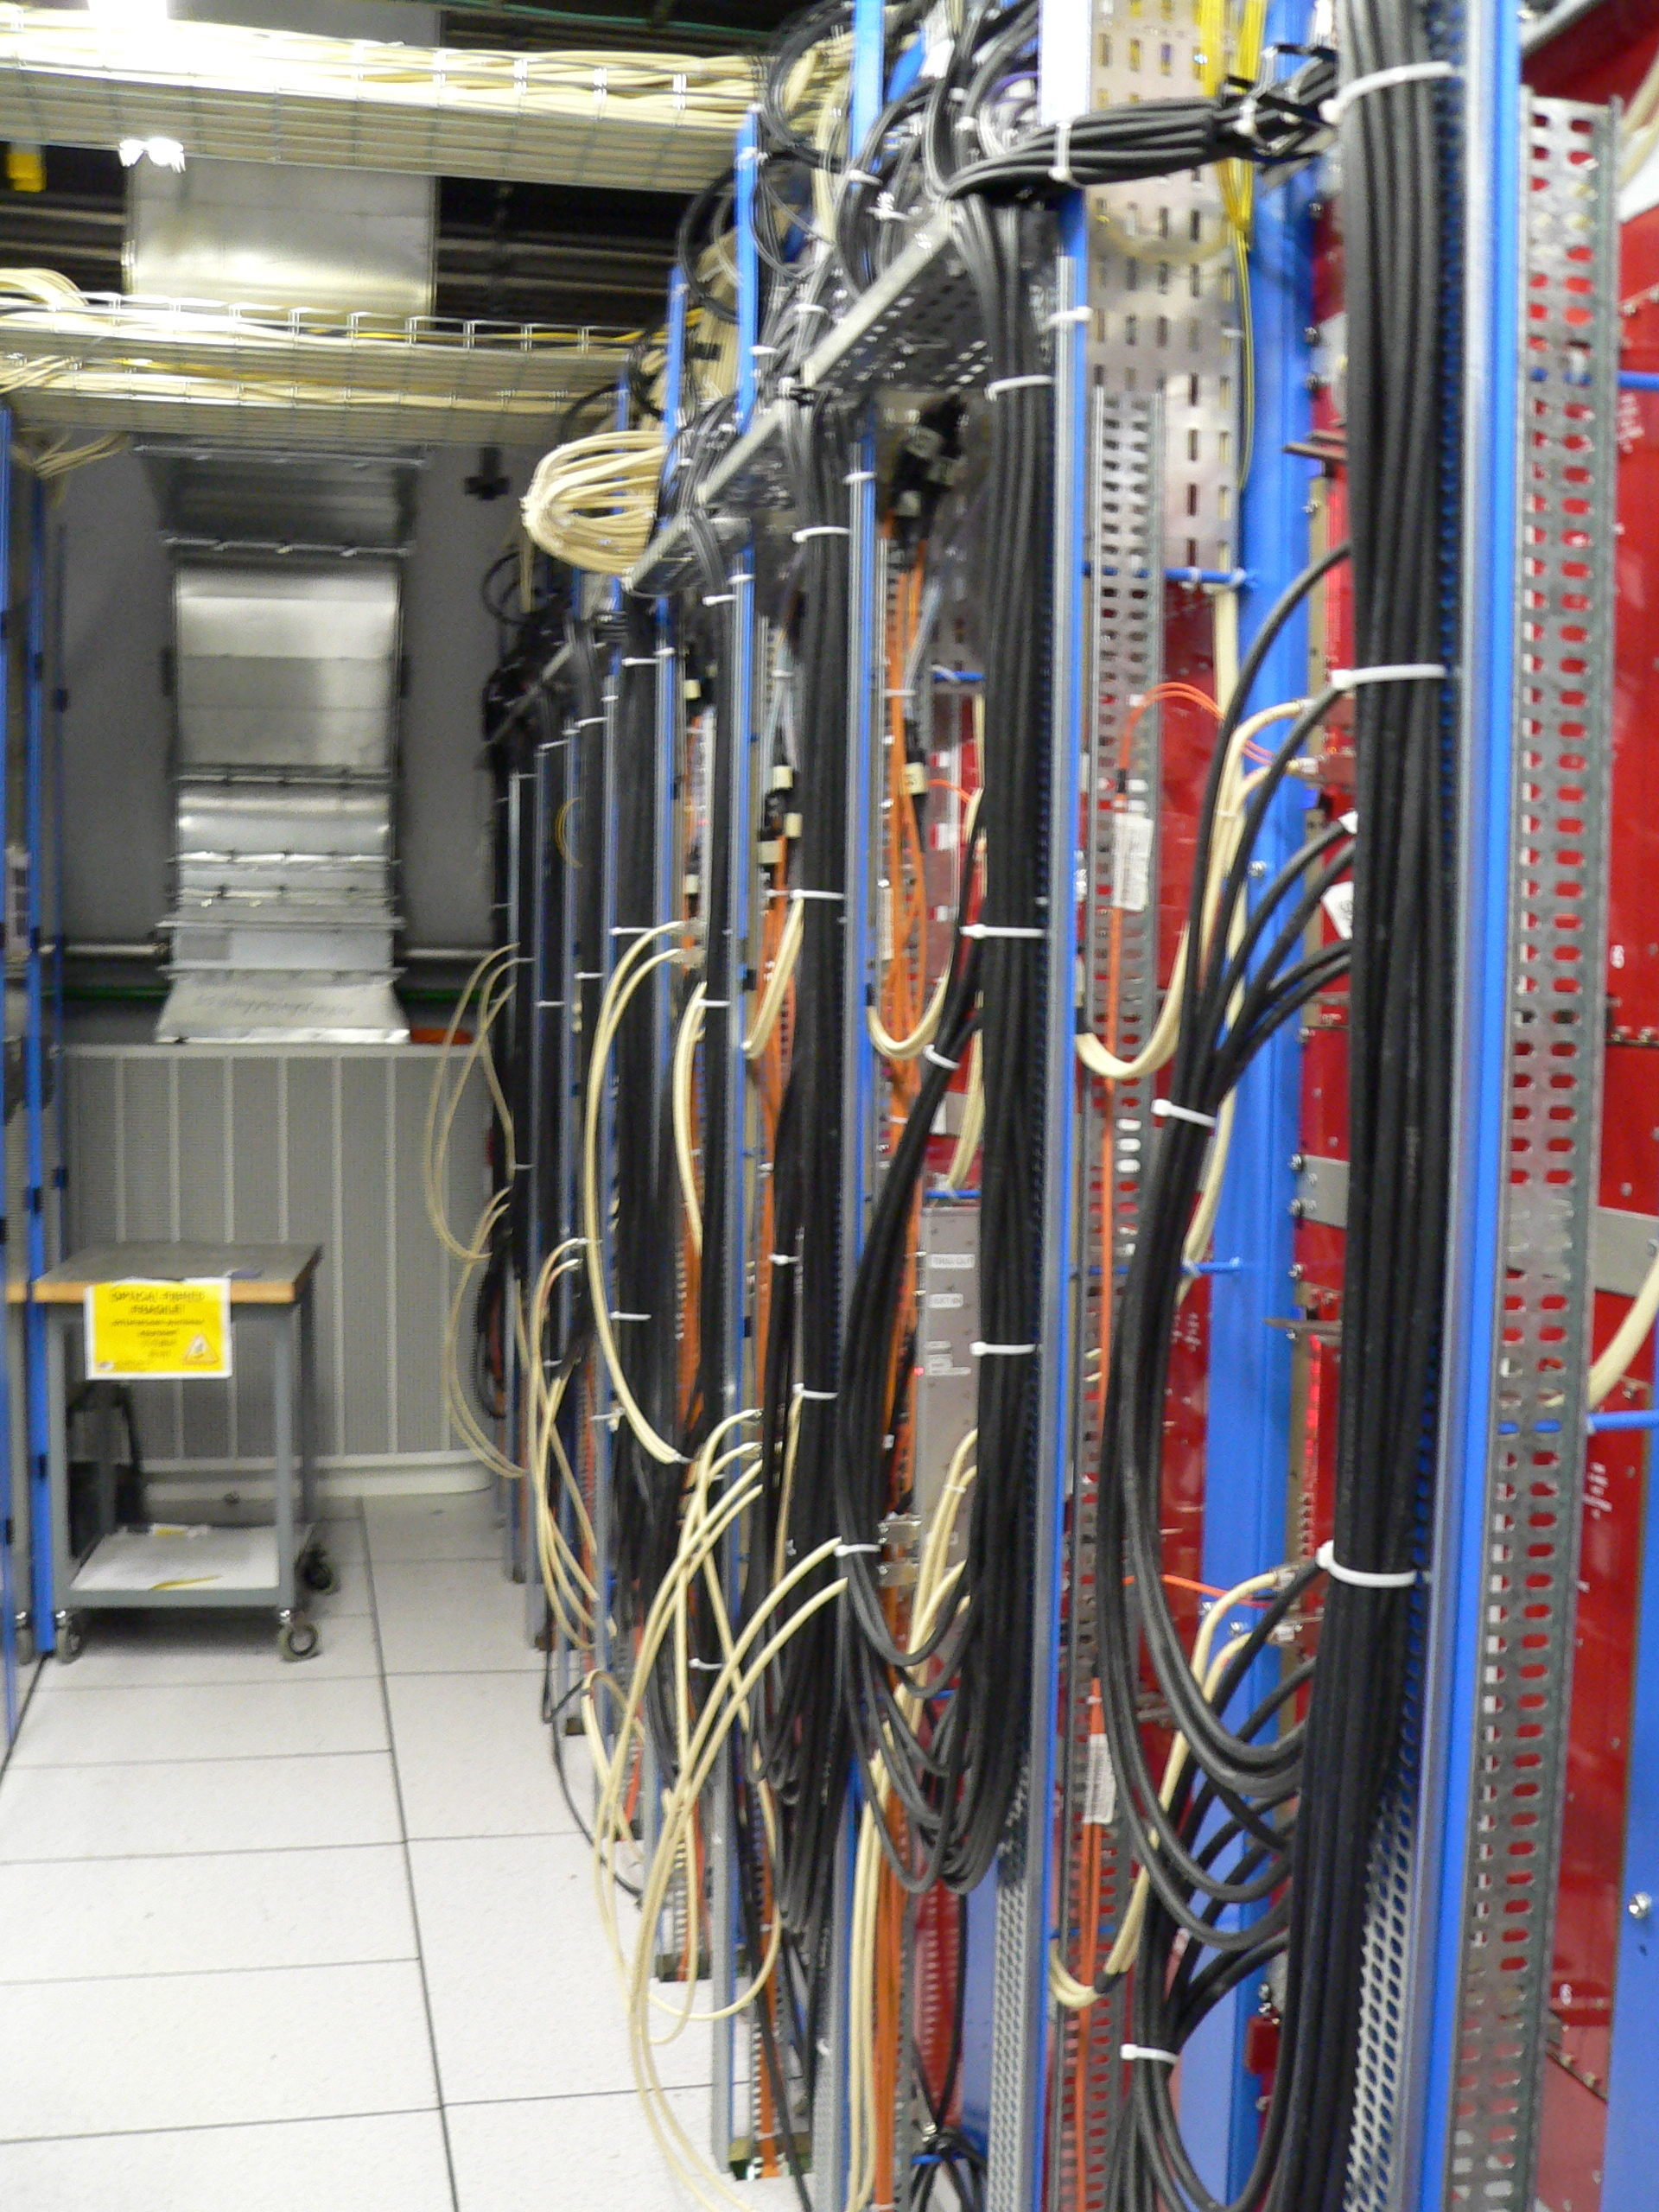
\includegraphics[width=.3\textwidth,height=.4\textheight]{TalkPics/sgs120315/L1.jpg}
          };
          \node[node distance=4cm,right of=l1node] (hltnode){
          };
          \node[node distance=1cm,above of=hltnode] (hlt2node){
            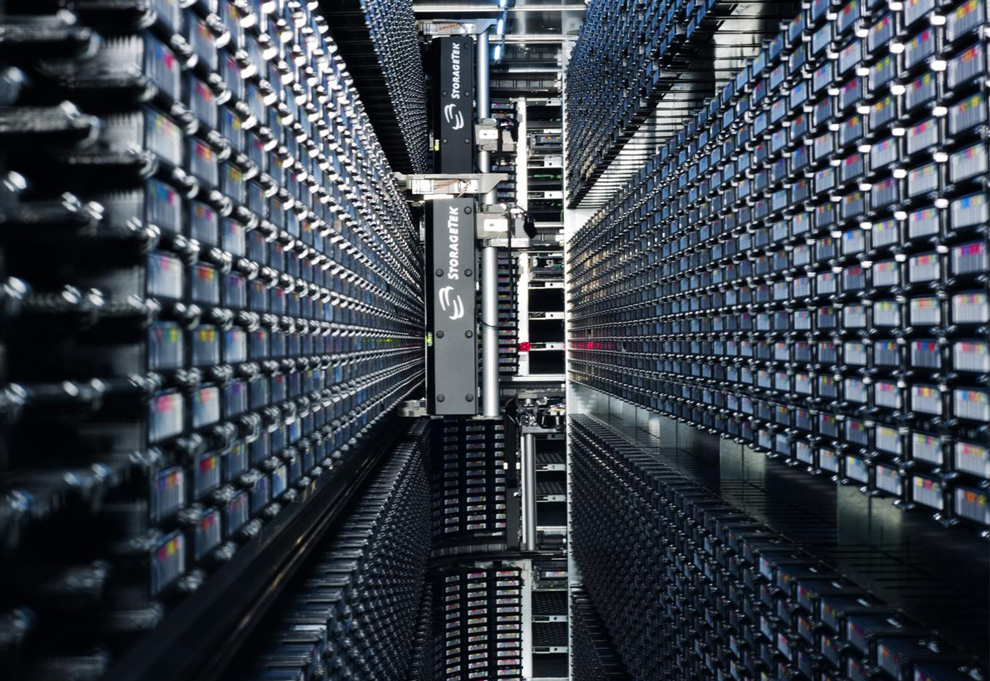
\includegraphics[width=.3\textwidth,height=.2\textheight]{TalkPics/RHULSeminar051016/tumblr_ktfo5h8L241qzyhb5o1_1280.jpg}
          };
        \node[node distance=1cm,below of=hltnode] (hlt3node){
            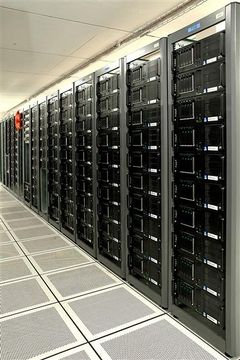
\includegraphics[width=.3\textwidth,height=.2\textheight]{TalkPics/sgs120315/HLT.jpg}
          };
          \node[node distance=4cm,right of=hltnode] (gridnode){
            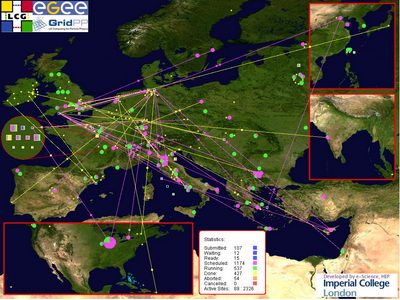
\includegraphics[width=.3\textwidth]{TalkPics/sgs120315/grid.jpg}
          };
        \node at (l1node.north) {\color{beamer@icmiddleblue}{Trigger}};
        \node at (hlt2node.north) {\color{beamer@icmiddleblue}{600 Hz stored on tape}};
        \node at (hlt3node.south) {\color{beamer@icmiddleblue}{Processing}};
        \node at (gridnode.north) {\color{beamer@icmiddleblue}{Analysis}};
        \node at (l1node.south) {\color{beamer@icmiddleblue}{40MHz $\rightarrow$ 1kHz}};
        \path[->,color=red,very thick] (1.4,-1) edge (2.4,-1);
        \path[->,color=red,very thick] (5.4,-1) edge (6.4,0.15);
        \path[->,color=red,very thick] (1.4,1) edge (2.4,1);
        \path[dashed,->,color=red,very thick] (4.4,0.6) edge (4.4,-0.3);
      \end{tikzpicture}
    \end{columns}
  \end{frame}



  \begin{frame}
    \frametitle{Trigger}
      %table of cuts and a comment
      \begin{block}{}
        \begin{itemize}
        \item Require a pair of jets with VBF topology
        \item Also require large $E_{T}^{miss}$
        \item[-] Calculated ignoring muons to enable background estimation
        \item Thresholds vary through run periods
        \end{itemize}
        \centering
        %% \begin{tabular}{l|c}
        %%   \hline
        %%   Variable & Requirement \\
        %%   \hline
        %%   Jet $p_{T}$ & $>$30-40 GeV\\
        %%   Dijet mass ($M_{jj}$) & $>$600-800 GeV \\
        %%   $\Delta\eta_{jj}$ & $>3.5$\\
        %%   $E_{T}^{miss}$ & $>40-65$ GeV\\
        %%   \hline
        %% \end{tabular}
      \end{block}
      \centering
      \includegraphics[clip=true,trim=0 0 0 50,width=.45\textwidth]{../../Thesis/plots/prompt/TrigEff_SingleMu_Jet2Pt.pdf}
      \includegraphics[clip=true,trim=0 0 0 50,width=.45\textwidth]{../../Thesis/plots/prompt/TrigEff_SingleMu_MET.pdf}
  \end{frame}

  %??maybe efficiency measurement
  \begin{frame}
    \frametitle{Trigger Efficiency Measurement}
    \begin{block}{}
      \begin{itemize}
      \item Trigger thresholds are a limiting factor for the analysis
      \item Need to measure accurately so turn on region can be used
      \item[-] Variables are highly correlated so measured by fitting as a function of $E_{T}^{miss}$ in bins of $M_{jj}$ and second jet $p_{T}$
      \end{itemize}
    \end{block}
          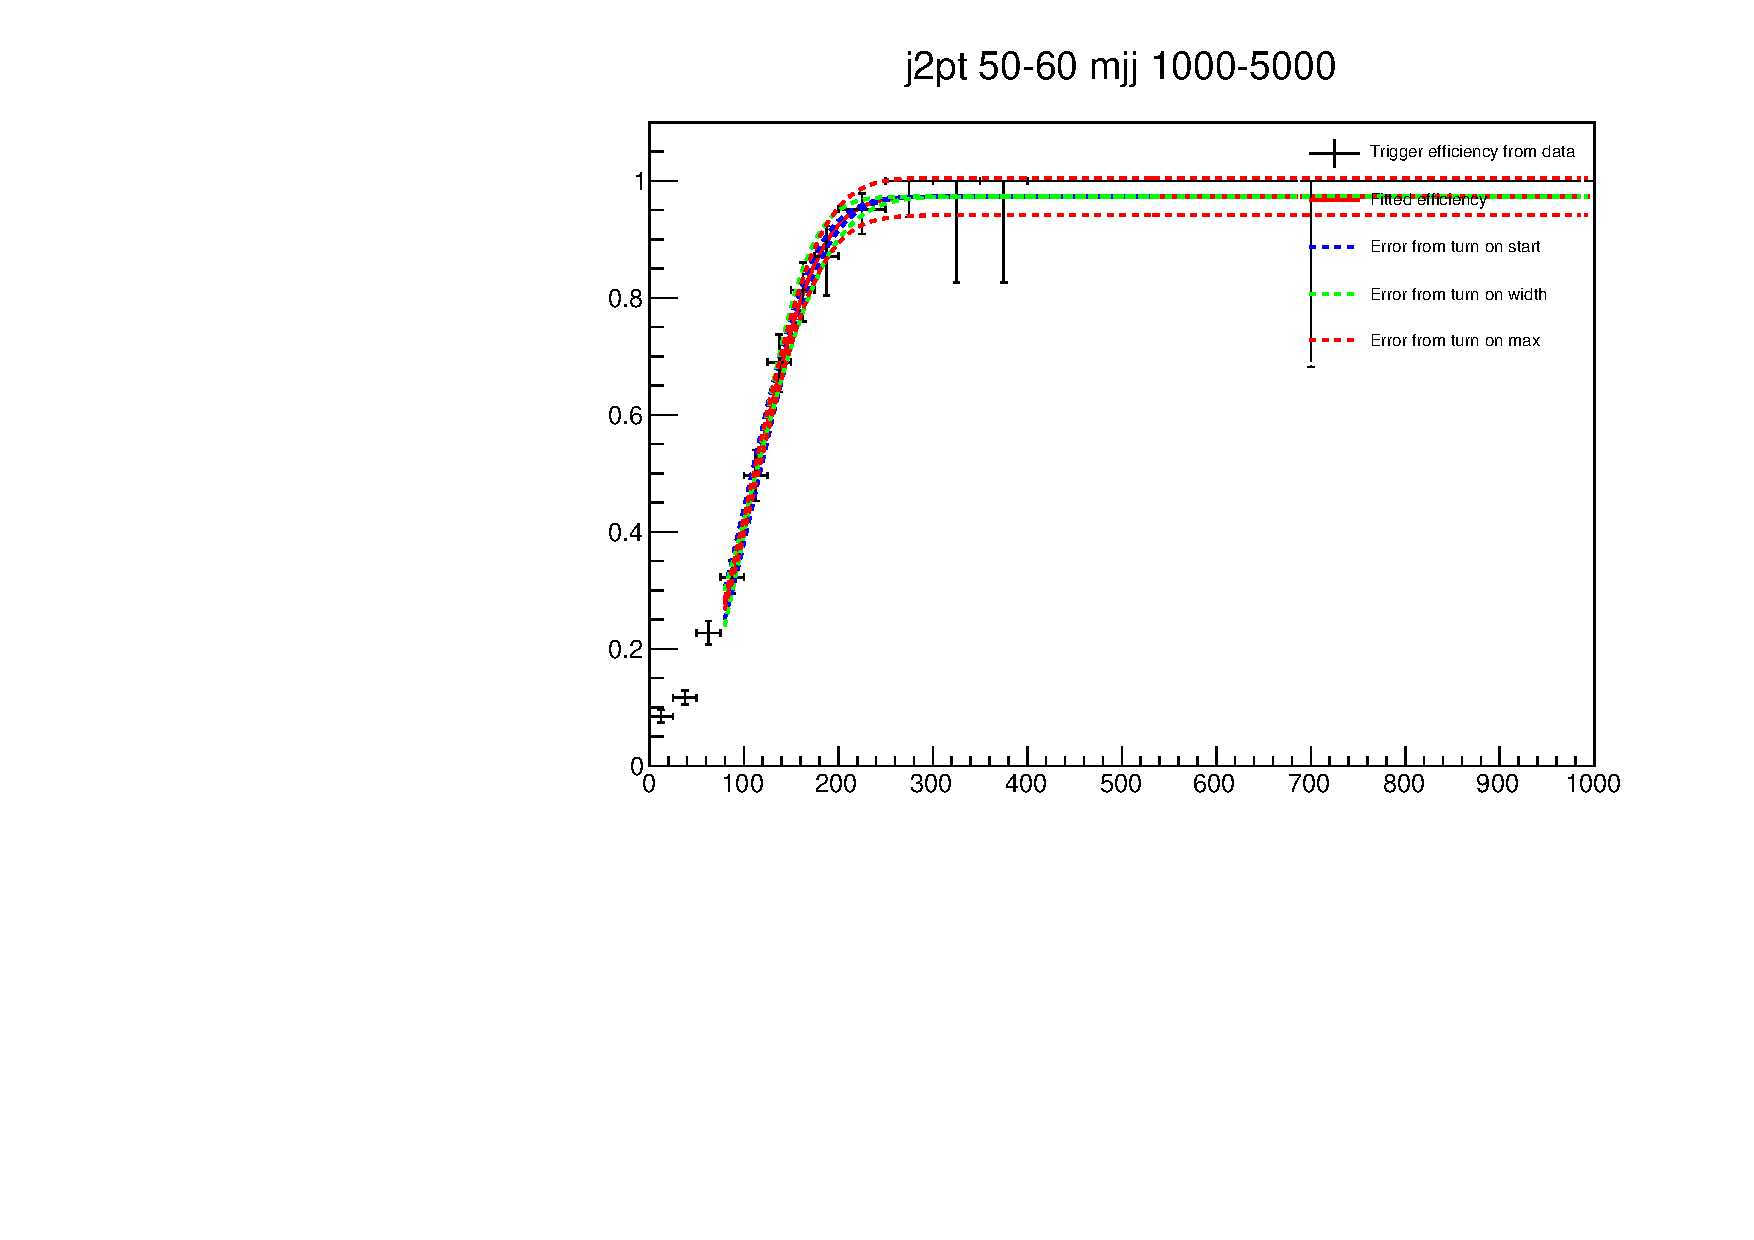
\includegraphics[width=.5\textwidth]{../../Thesis/plots/parked/AN-14-243-figs/trigfitplots/hData_MET_1D_35D.pdf}
          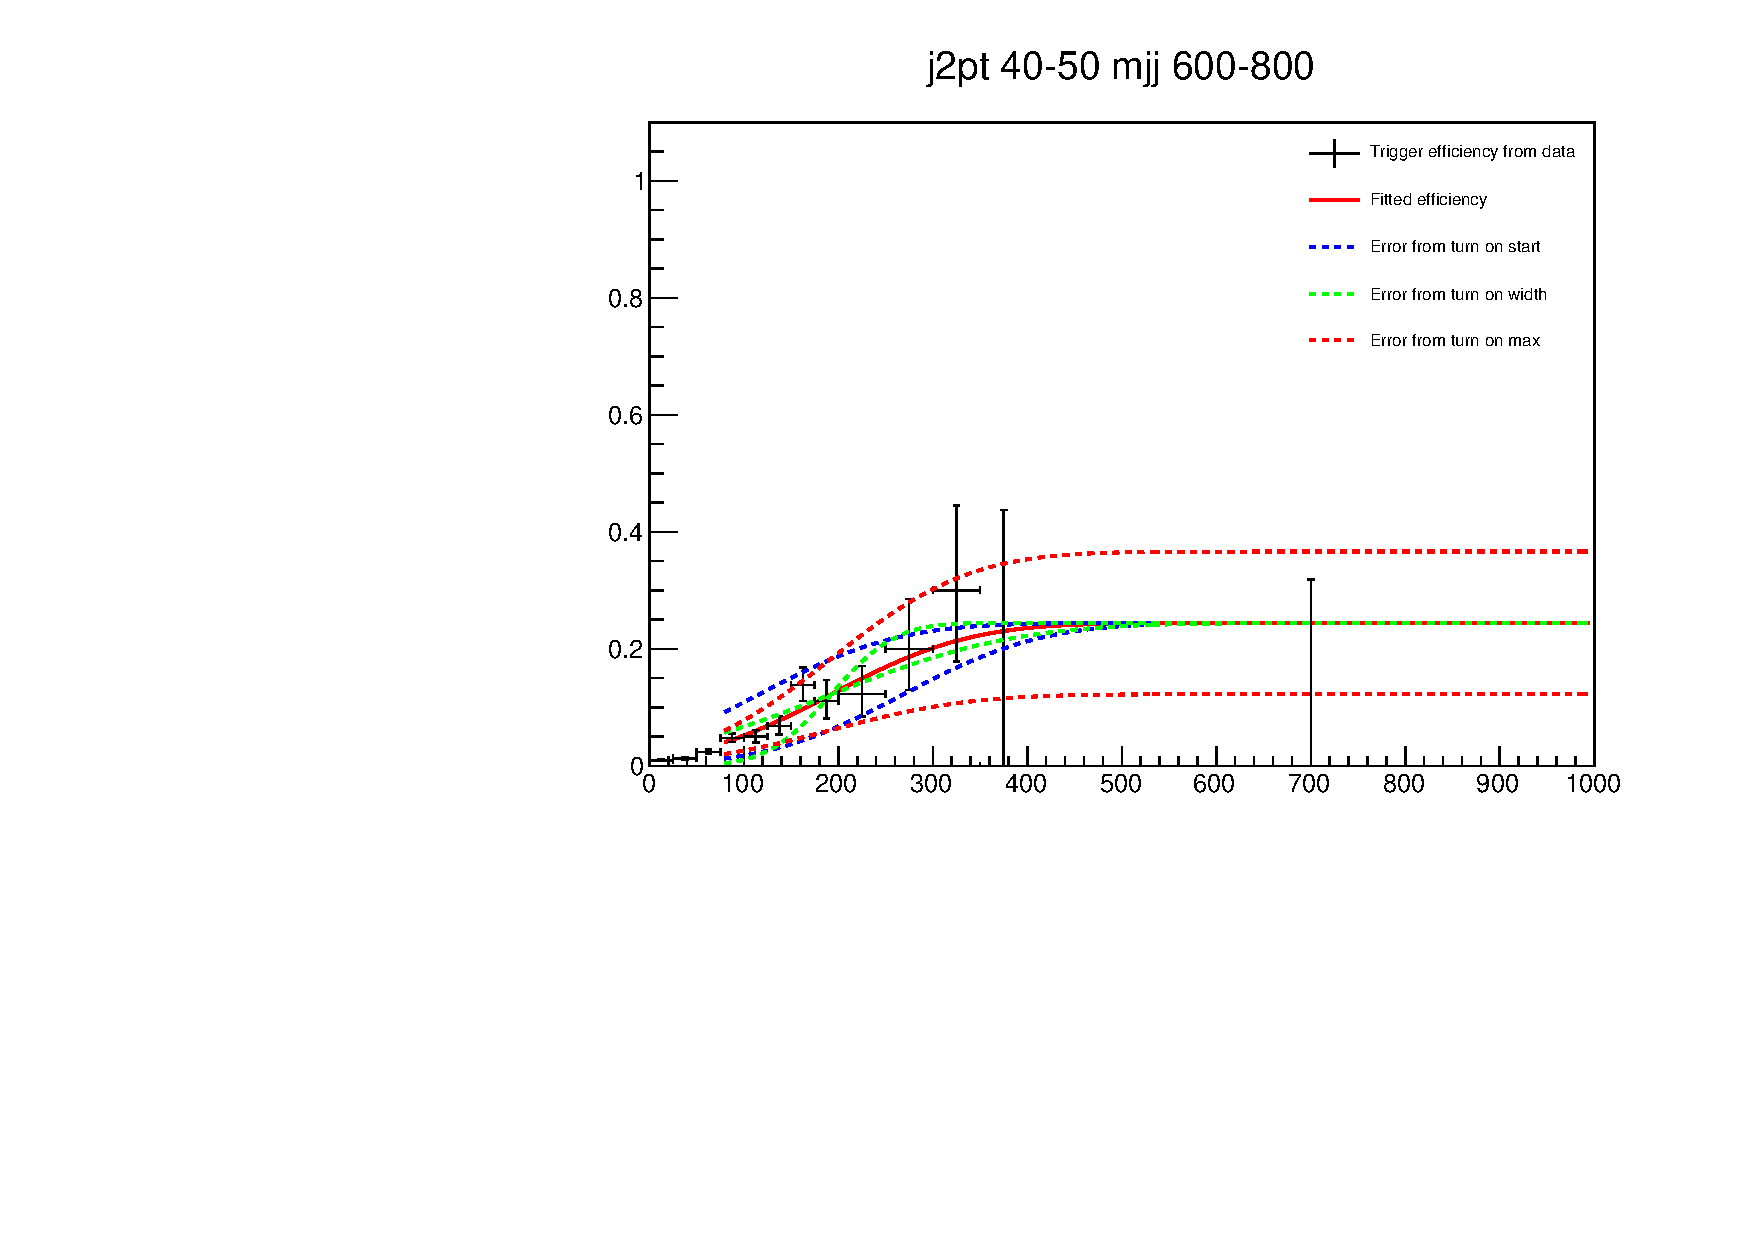
\includegraphics[width=.5\textwidth]{../../Thesis/plots/parked/AN-14-243-figs/trigfitplots/hData_MET_1D_22D.pdf}

  \end{frame}


  %Selection: preselection variables
  \begin{frame}
    \frametitle{Preselection}
    \begin{columns}
      \column{.5\textwidth}
      \begin{block}{}
        \begin{itemize}
        \item After setting trigger variables to point of 50\% trigger efficiency most data is still QCD
        \item Not modelled well by MC
        \item[-] Rate is too high to produce a large enough sample
        \item Additional tight cuts must be applied before MC driven selection optimisation can be performed
        \end{itemize}
      \end{block}
      \column{.5\textwidth}
      \centering
      \includegraphics[width=.8\textwidth]{../../Thesis/plots/parked/AN-14-243-figs/lognopreselnunu_metnomu_significance.pdf}

      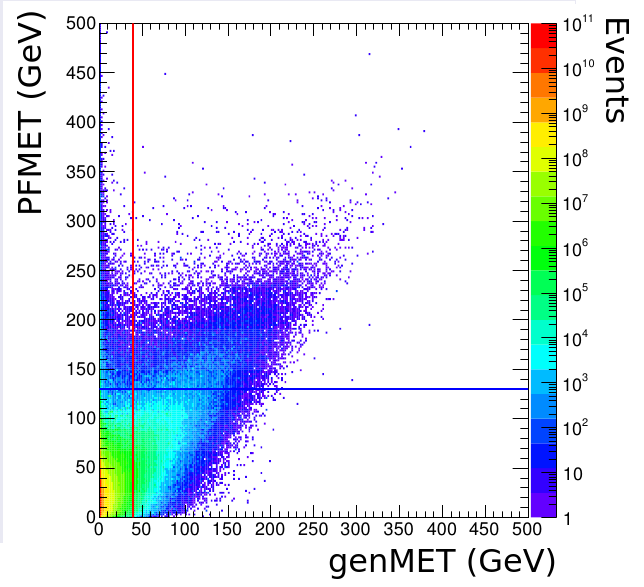
\includegraphics[width=.8\textwidth]{../../Thesis/plots/parked/AN-14-243-figs/Joao_140209_p11.png}
    \end{columns}
  \end{frame}

  \begin{frame}
    \frametitle{Reducing QCD Backgrounds}
    %WJETS                                                                                                                                                                                                                                  
      \begin{block}{$E_{T}^{miss}$ significance}
        \centering
        \begin{fmfgraph*}(60,50)
          \fmftop{i1,m1,m2,m3,m4,m5,m6,m7,o1}
          \fmfbottom{i2,m8,m9,m10,m11,o2}
          \fmf{fermion,tension=4}{v1,i2}
          \fmf{fermion,tension=4}{v1,o2}
          \fmf{fermion,label=$jets$,label.side=left}{v1,m1}
          \fmf{dashes}{v1,m3}
          \fmf{fermion}{v1,m4}
          \fmf{fermion}{v1,m5}
          \fmf{fermion}{v1,m6}
          \fmf{fermion}{v1,m7}
          \fmf{fermion}{v1,m8}
          \fmf{fermion}{v1,m9}
          \fmf{fermion}{v1,m10}
          \fmf{fermion}{v1,m11}
          \fmflabel{$jet$}{i2}
          \fmflabel{$jet$}{o2}
        \end{fmfgraph*}
        \hspace{1.5cm}
        VS
        \hspace{1.5cm}
        \begin{fmfgraph*}(60,50)
          \fmftop{i1,m1,m2,m3,m4,m5,m6,m7,o1}
          \fmfbottom{i2,m8,m9,m10,m11,o2}
          \fmf{fermion,tension=4}{v1,i2}
          \fmf{fermion,tension=4}{v1,o2}
          \fmf{fermion,label=$jets$,label.side=left}{v1,m1}
          \fmf{dashes}{v1,m3}
          \fmflabel{$jet$}{i2}
          \fmflabel{$jet$}{o2}
        \end{fmfgraph*}
        \vspace{.2cm}
      \end{block}
      \begin{block}{min$\Delta\phi$(j,$E_{T}^{miss}$)}
        \centering
        \begin{fmfgraph*}(60,50)
          \fmftop{i1,m1,m2,m3,m4,m5,m6,m7o1}
          \fmfbottom{i2,o2}
          \fmf{fermion,tension=4}{v1,i2}
          \fmf{fermion,tension=4}{v1,o2}
          \fmf{fermion,label=$jets$,label.side=left}{v1,m1}
          \fmf{dashes}{v1,m2}
          \fmflabel{$jet$}{i2}
          \fmflabel{$jet$}{o2}
        \end{fmfgraph*}
        \vspace{.2cm}
      \end{block}


  \end{frame}

  \begin{frame}
    \frametitle{Preselection}
    \begin{block}{}
      \begin{itemize}
      \item Require $E_{T}^{miss}$ significance$>4$, min$\Delta\phi$(j,$E_{T}^{miss}$)$>2$ and $M_{jj}>800$ GeV
      \end{itemize}
    \end{block}
    \begin{tikzpicture}
      \node[anchor=south west,inner sep=0] (image) at (0,0) { \begin{columns}\column{.5\textwidth}      \begin{block}{\scriptsize Before} \includegraphics[width=\textwidth]{../../Thesis/plots/parked/AN-14-243-figs/lognopreselnunu_metnomu_significance.pdf} \end{block}
    \column{.5\textwidth} \begin{block}{\scriptsize After}  \includegraphics[width=\textwidth]{../../Thesis/plots/parked/AN-14-243-figs/logmjj800nunu_dijet_M.pdf} \end{block} \end{columns} };
      \begin{scope}[x={(image.south east)},y={(image.north west)}]
        \path[->,color=red,ultra thick] (0.3,0.5) edge (0.6,0.5);
      \end{scope}
    \end{tikzpicture}
  \end{frame}

  %Strategy after trigger
  \begin{frame}
    \frametitle{Remaining backgrounds}
    \begin{block}{}
      \begin{itemize}
      \item After preselection most backgrounds are from $W$/$Z$+jets
      \item Veto leptons to reduce leptonic decay contribution
      \item Hadronic decays reduced by anti-QCD selection
      \item Apply further selection then estimate remainder with data driven techniques
      \item[-] Further minor contributions from VV, top and remaining QCD          
      \end{itemize}
    \end{block}
    
    \begin{columns}
      \column{.33\textwidth}
      \begin{block}{W+jets}
        \centering
        \begin{fmfgraph*}(60,50)
          \fmftop{i1,m1,m2,o1}
          \fmfbottom{i2,o2}
          \fmf{fermion,label=$e/\mu/\tau$,label.side=left}{v2,m1}
          \fmf{fermion,label=$\nu$,label.side=right}{v2,m2}
          \fmf{photon,tension=7/5,label=$W$}{v1,v2}
          \fmf{fermion}{v1,i2}
          \fmf{fermion}{v1,o2}
          \fmflabel{$jet$}{i2}
          \fmflabel{$jet$}{o2}
        \end{fmfgraph*}
        \vspace{.2cm}
      \end{block}

      \column{.33\textwidth}
      \begin{block}{Z+jets}
        \centering
        \begin{fmfgraph*}(60,50)
          \fmftop{i1,m1,m2,o1}
          \fmfbottom{i2,o2}
          \fmf{fermion}{v1,i2}
          \fmf{fermion}{v1,o2}
          \fmf{photon,tension=7/5,label=$Z$}{v1,v2}
          \fmf{fermion,label=$\nu$,label.side=left}{v2,m1}
          \fmf{fermion,label=$\nu$,label.side=right}{v2,m2}
          \fmflabel{$jet$}{i2}
          \fmflabel{$jet$}{o2}
        \end{fmfgraph*}
        \vspace{.2cm}
      \end{block}
    \end{columns}
    
  \end{frame}

  \begin{frame}
    \frametitle{Data driven background estimation}
      \vspace{-.3cm}
      \begin{block}{}
        \scriptsize
        \begin{itemize}
          \item Choose control region enriched in background
          \item Use MC signal-control ratio to go to signal region:
          $N^{signal}_{Bkg} = \frac{(N^{control}_{obs}-N^{control}_{other bkgs})}{N^{signal}_{MC}}\cdot N^{control}_{MC}.$
          \item Ratio referred to as data driven scale factor
        \end{itemize}
      \end{block}
    \begin{tikzpicture}
      \node[anchor=south west,inner sep=0] (image) at (0,0) { \begin{columns}\column{.5\textwidth}      \begin{block}{\scriptsize Control Region: Single Muon} 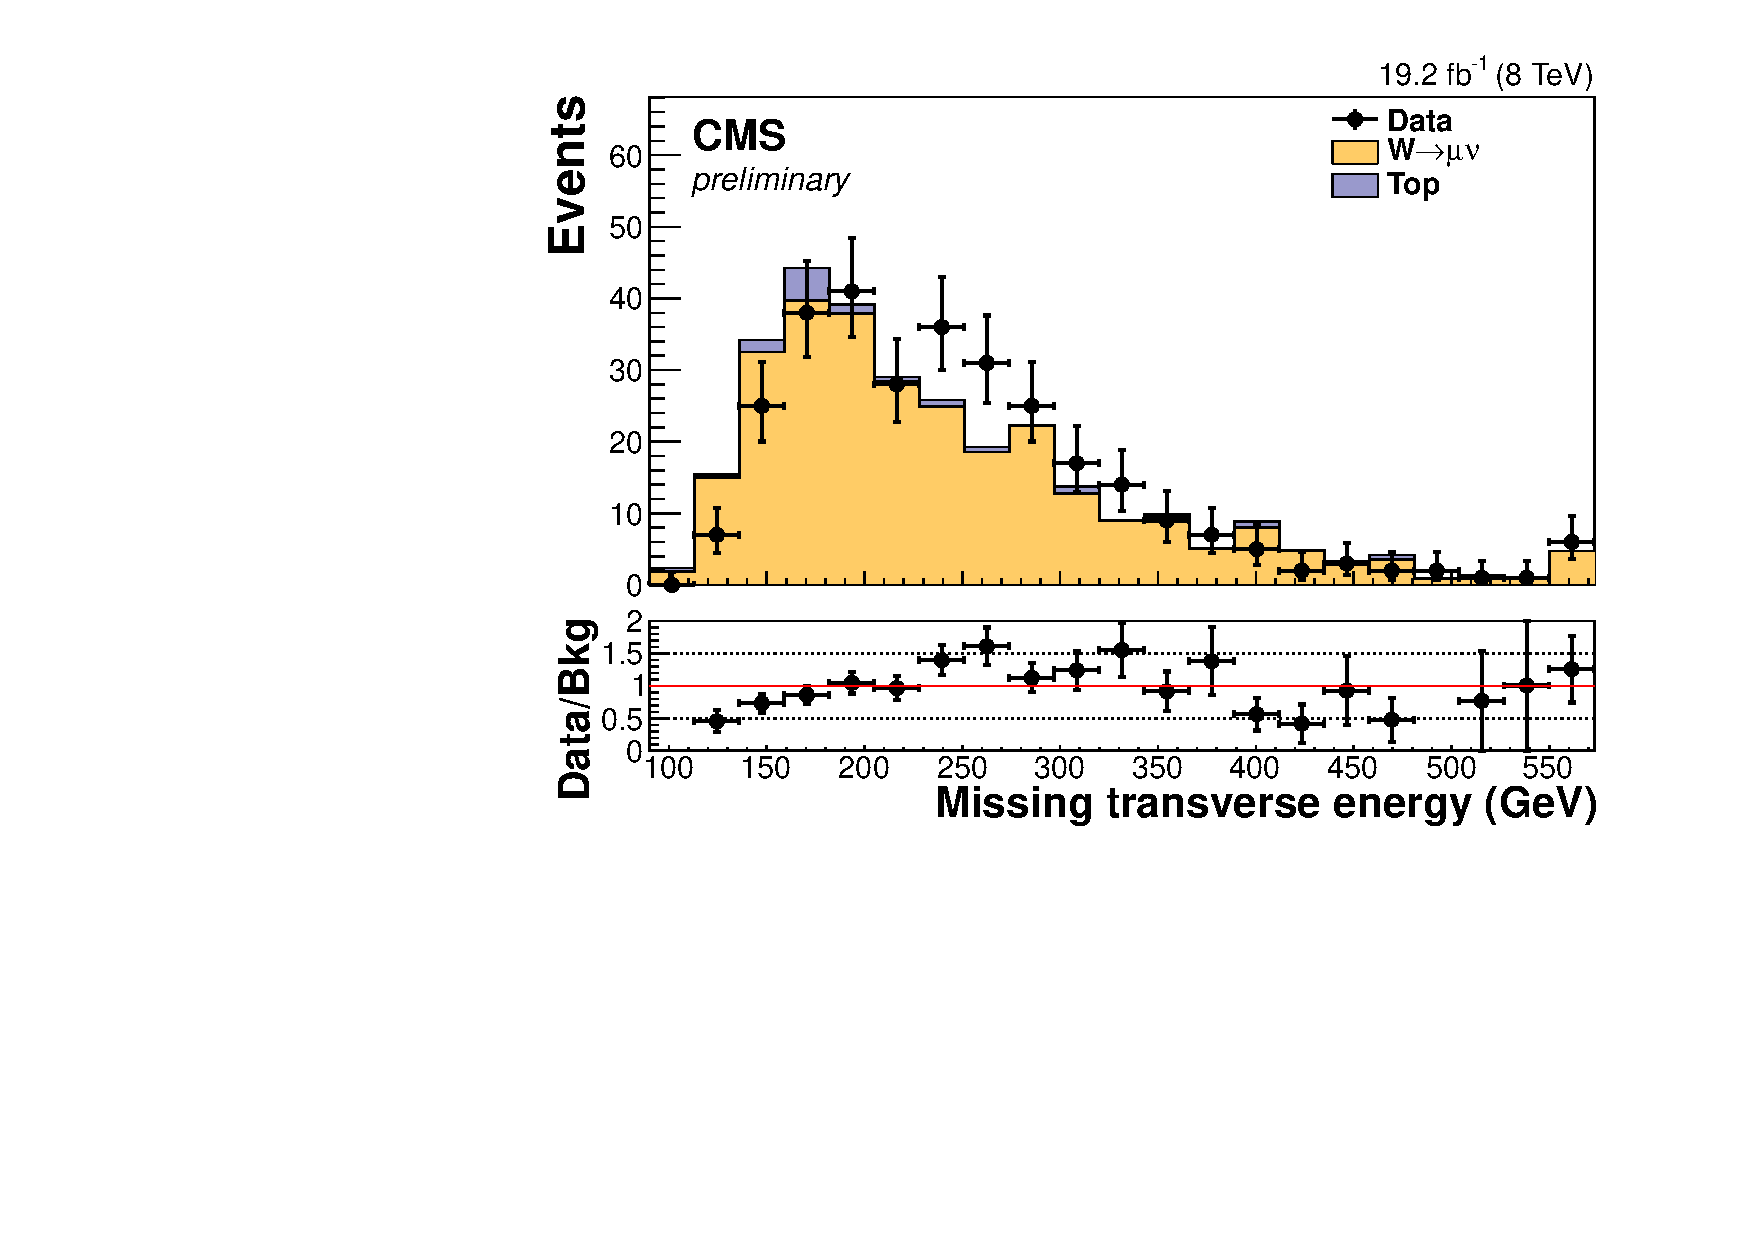
\includegraphics[width=\textwidth]{TalkPics/studentseminar221015/hig14038figures/output_sigreg/munu_metnomuons.pdf} \end{block}
    \column{.5\textwidth} \begin{block}{\scriptsize Signal Region: Lepton veto}  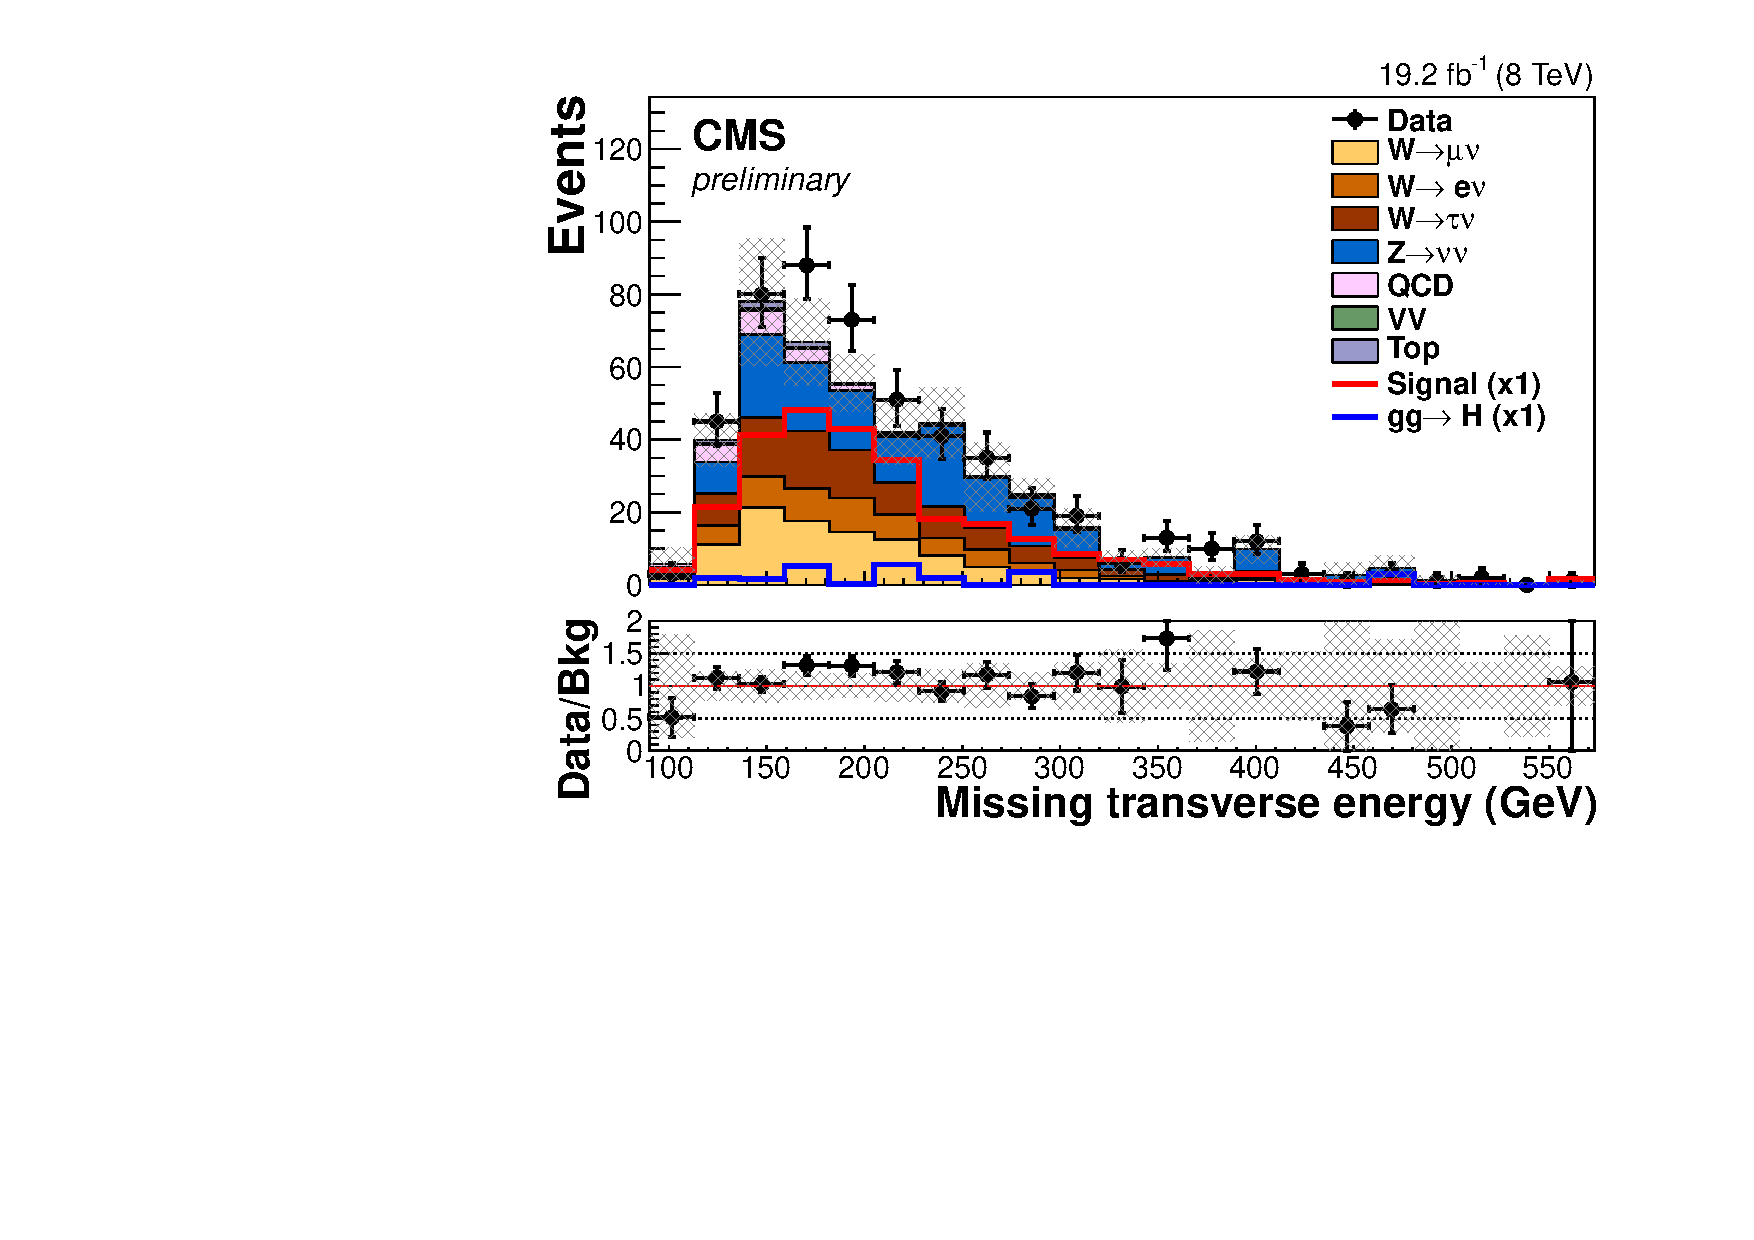
\includegraphics[width=\textwidth]{TalkPics/studentseminar221015/hig14038figures/output_sigreg/nunu_metnomuons.pdf} \end{block} \end{columns} };
      \begin{scope}[x={(image.south east)},y={(image.north west)}]
        \path[->,color=red,ultra thick] (0.3,0.5) edge (0.6,0.5);
      \end{scope}
    \end{tikzpicture}

  \end{frame}


  %Remaining background estimation W/Z
  \begin{frame}
    \frametitle{W control regions}
    \begin{block}{}
      \begin{itemize}
      \item For $W\rightarrow\ell\nu$+jets background use region with inverted lepton veto
      \item[-] Single electron region for $W\rightarrow e\nu$
      \end{itemize}
    \end{block}
    \begin{block}{$W\rightarrow e\nu$}
    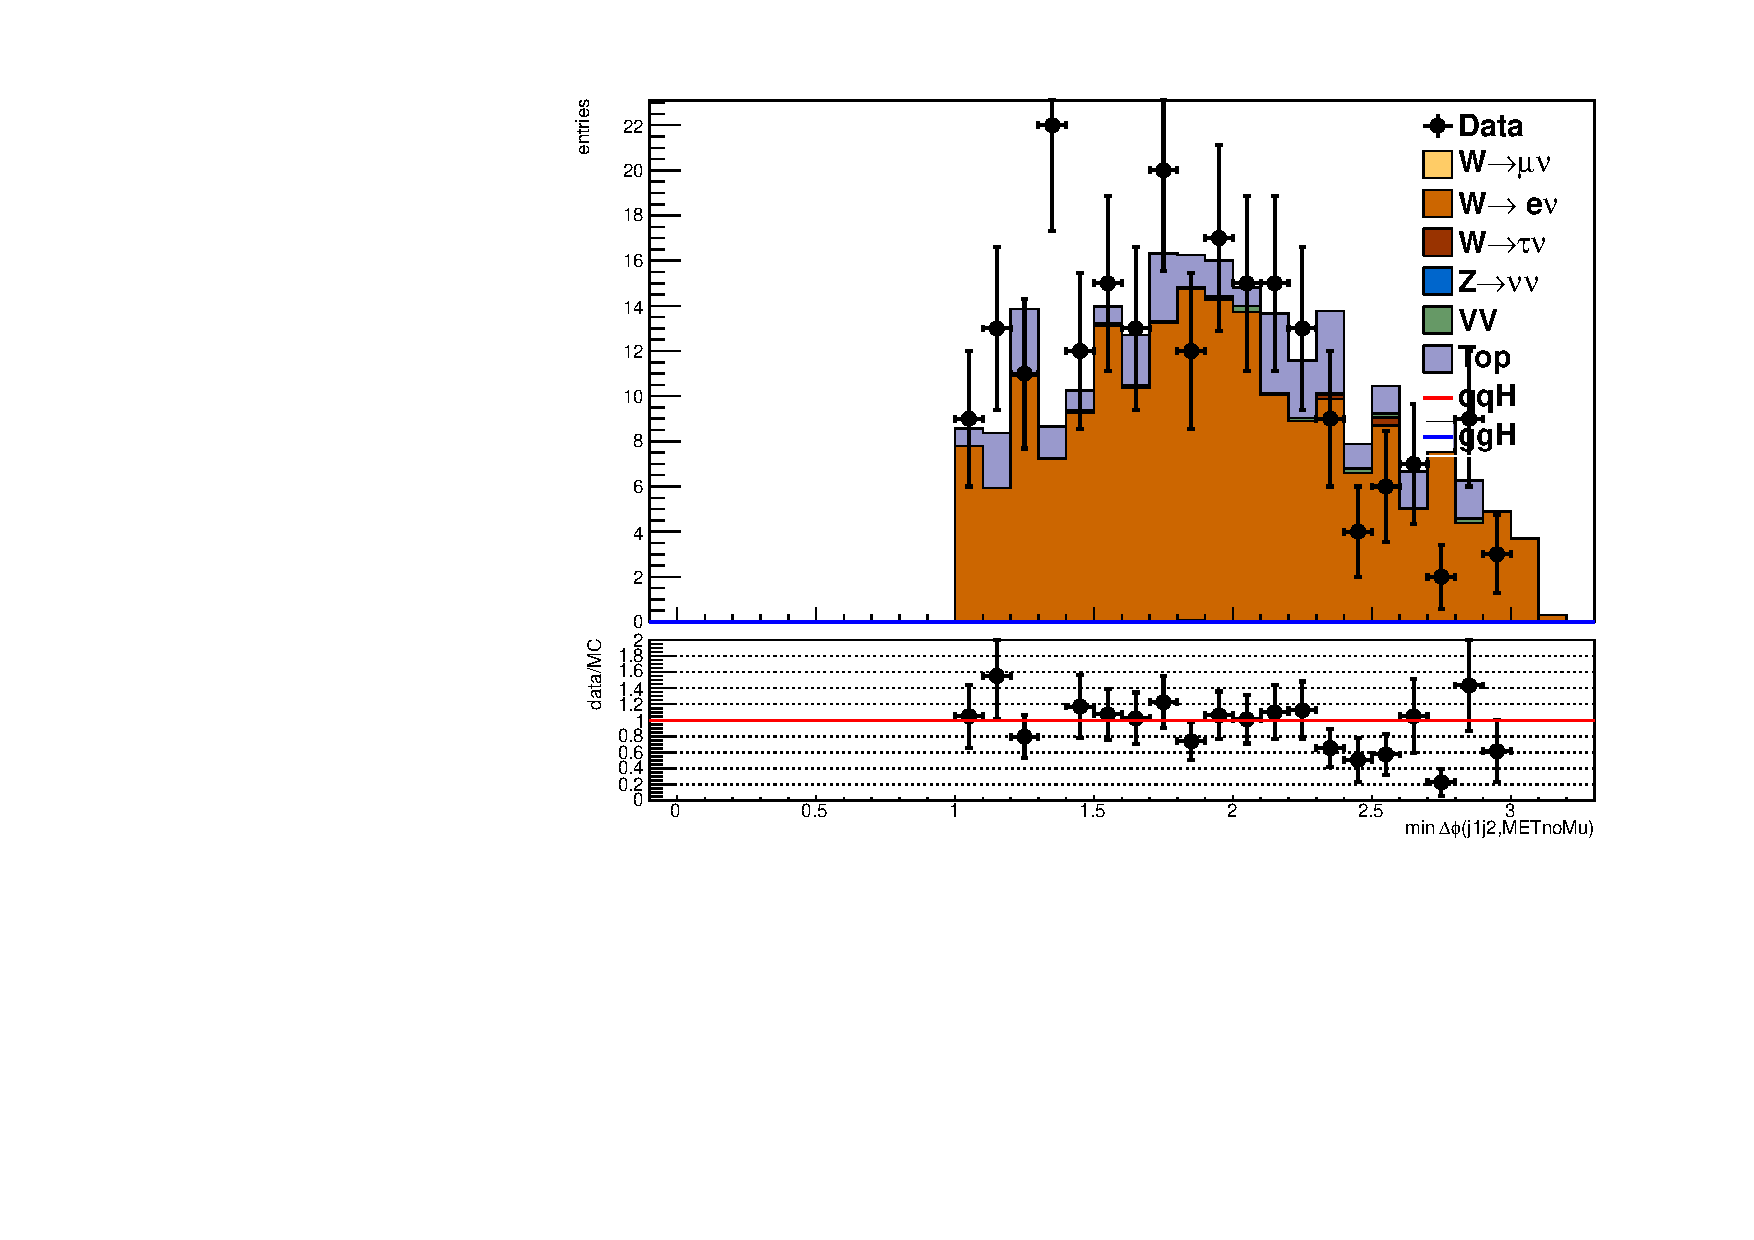
\includegraphics[width=.5\textwidth]{../../Thesis/plots/parked/HIG-14-038-figs/output_sigreg/enu_jetmetnomu_mindphi.pdf}
    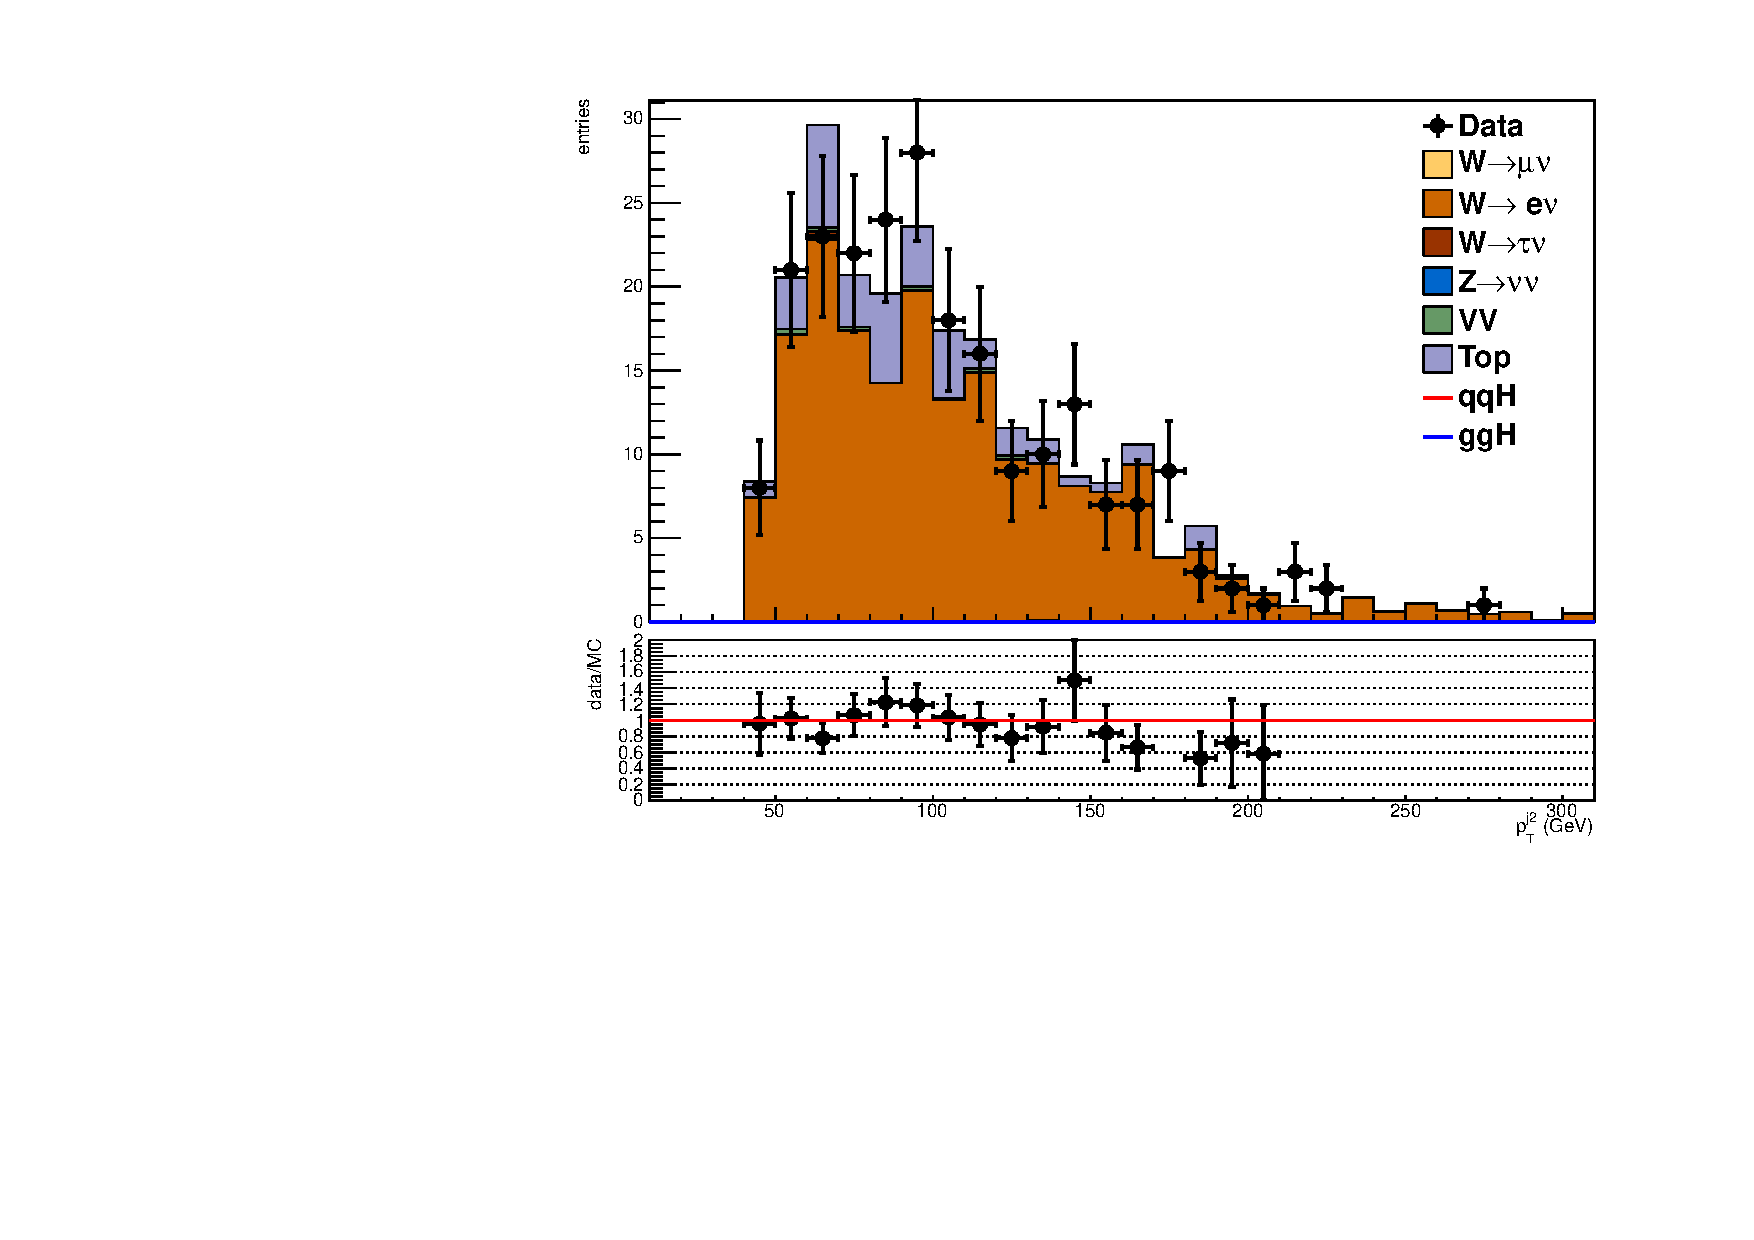
\includegraphics[width=.5\textwidth]{../../Thesis/plots/parked/HIG-14-038-figs/output_sigreg/enu_jet2_pt.pdf}
    \end{block}
  \end{frame}

  \begin{frame}
    \frametitle{W control regions}
    \begin{block}{}
      \begin{itemize}
      \item Single muon region for $W\rightarrow\mu\nu$ with $E_{T}^{miss}$ recalculated ignoring muon
      \end{itemize}
    \end{block}
    \begin{block}{$W\rightarrow \mu\nu$}
    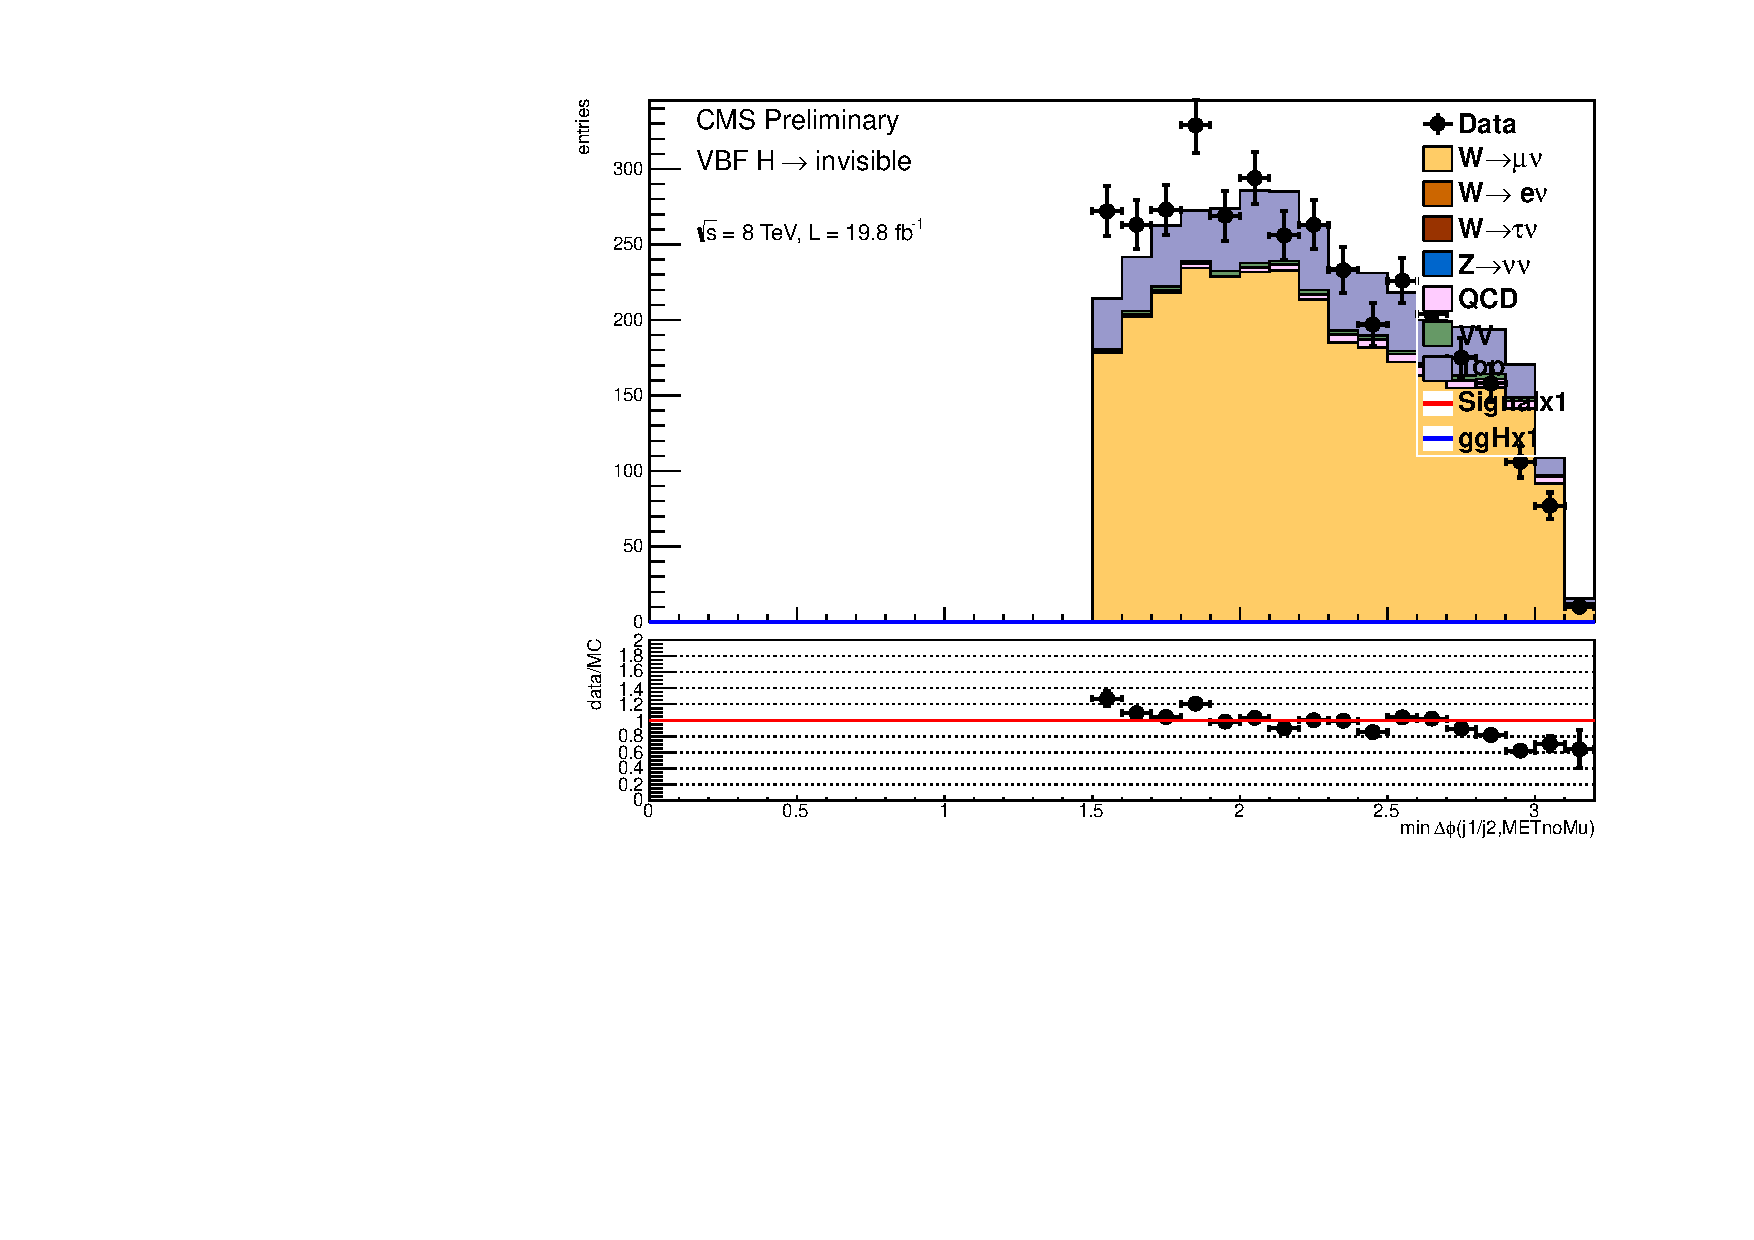
\includegraphics[width=.5\textwidth]{../../Thesis/plots/parked/HIG-14-038-figs/output_sigreg/munu_jetmetnomu_mindphi.pdf}
    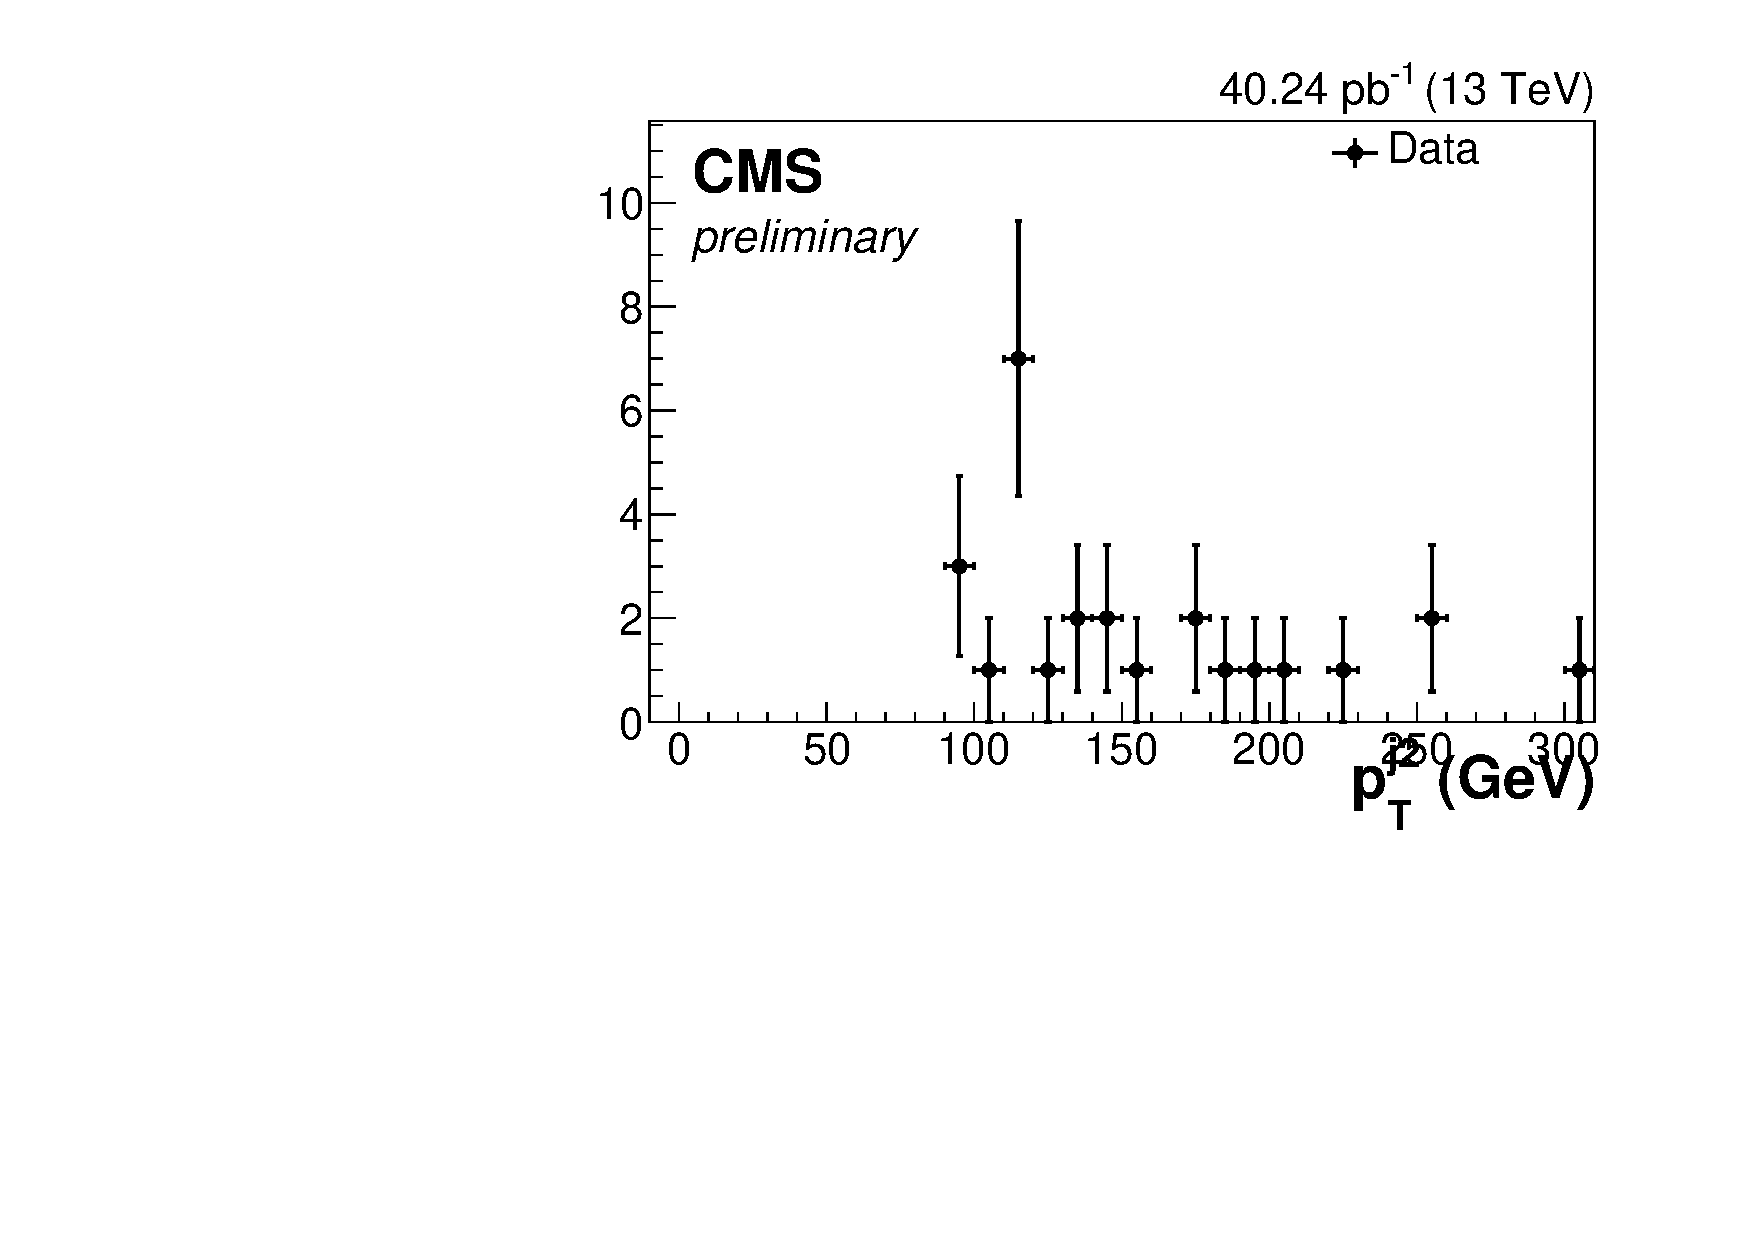
\includegraphics[width=.5\textwidth]{../../Thesis/plots/parked/HIG-14-038-figs/output_sigreg/munu_jet2_pt.pdf}
    \end{block}
  \end{frame}

  \begin{frame}
    \frametitle{W control regions}
    \vspace{-.2cm}
    \begin{block}{}
      \begin{itemize}
      \item Very few events in single tau region after other selections
      \item[-] Relaxed min$\Delta\phi$(j,$E_{T}^{miss}$) requirement to $>1$ only considering leading two jets
      \item[-] Added lepton-$E_{T}^{miss}$ $m_{T}>20$ GeV requirement to reduce QCD
      \end{itemize}
    \end{block}
    \vspace{-.15cm}
    \begin{block}{$W\rightarrow \tau\nu$}
    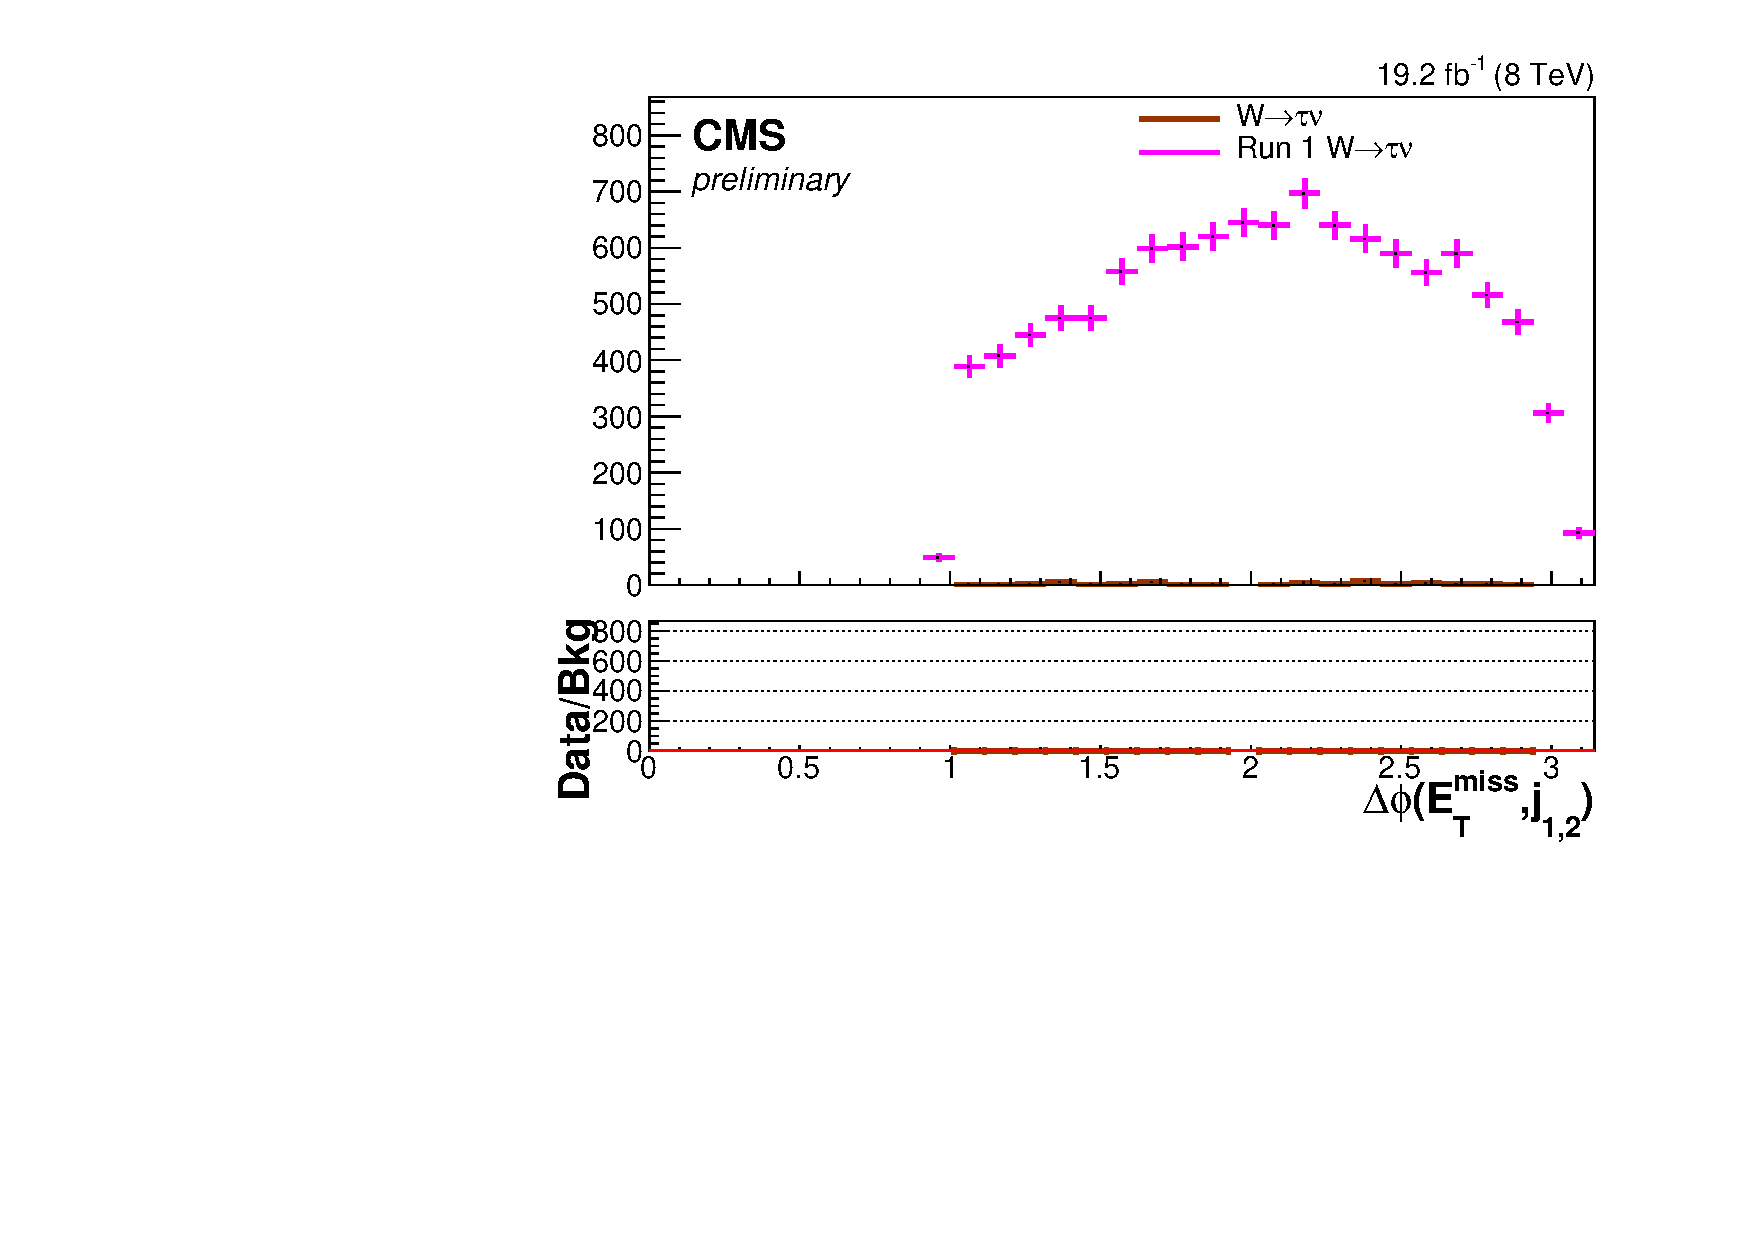
\includegraphics[width=.5\textwidth]{../../Thesis/plots/parked/HIG-14-038-figs/output_sigreg/taunu_jetmetnomu_mindphi.pdf}
    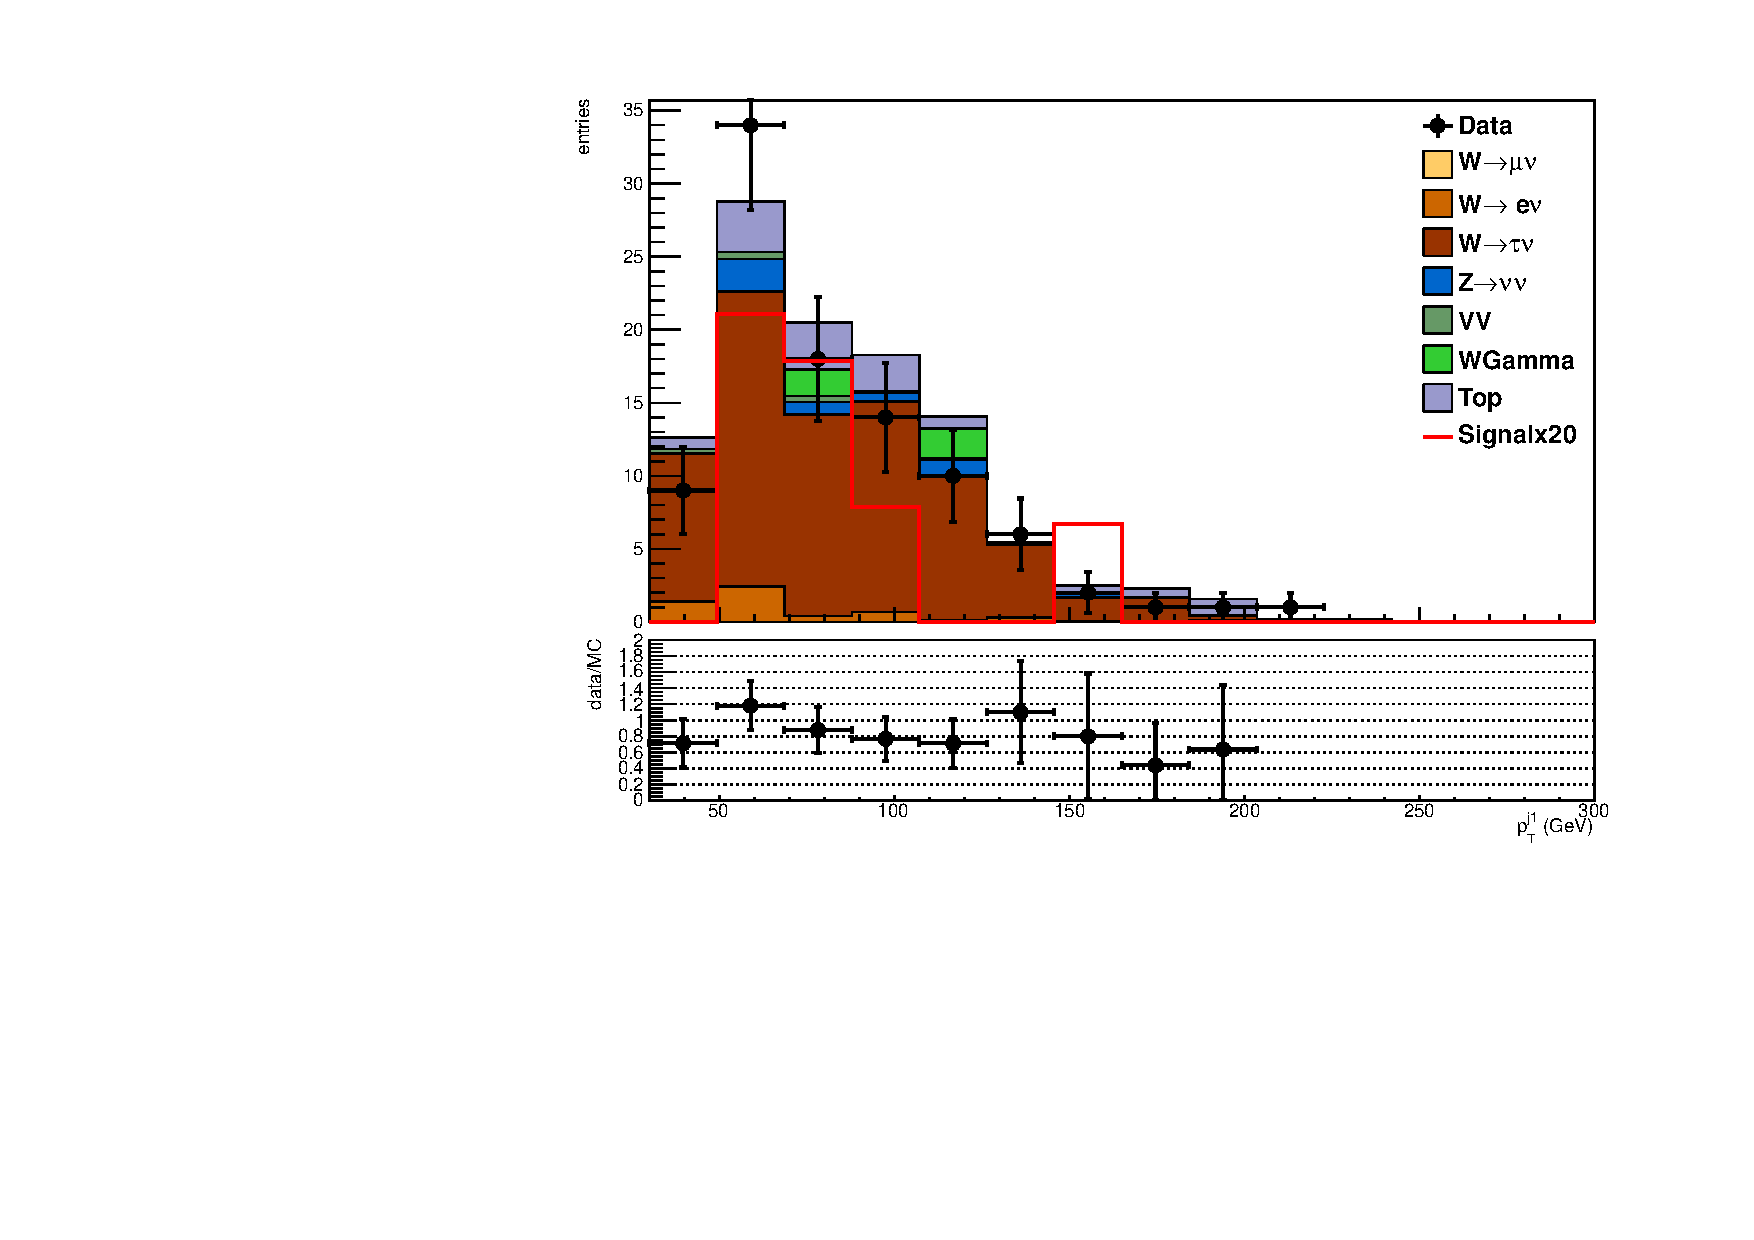
\includegraphics[width=.5\textwidth]{../../Thesis/plots/parked/HIG-14-038-figs/output_sigreg/taunu_jet2_pt.pdf}
    \end{block}
  \end{frame}

  \begin{frame}
    \frametitle{Z$\rightarrow\nu\nu$ control region}
    \vspace{-.2cm}
    \begin{block}{}
      \begin{itemize}
      \item Remove lepton veto and require a dimuon
      \item[-] Statistical uncertainty on event rate in this region is limiting uncertainty on the analysis
      \item $Z\rightarrow\nu\nu$ and $Z/\gamma^{*}\rightarrow\mu\mu$ have different cross-sections
      \item[-] Must be corrected for
      \end{itemize}
    \end{block}
    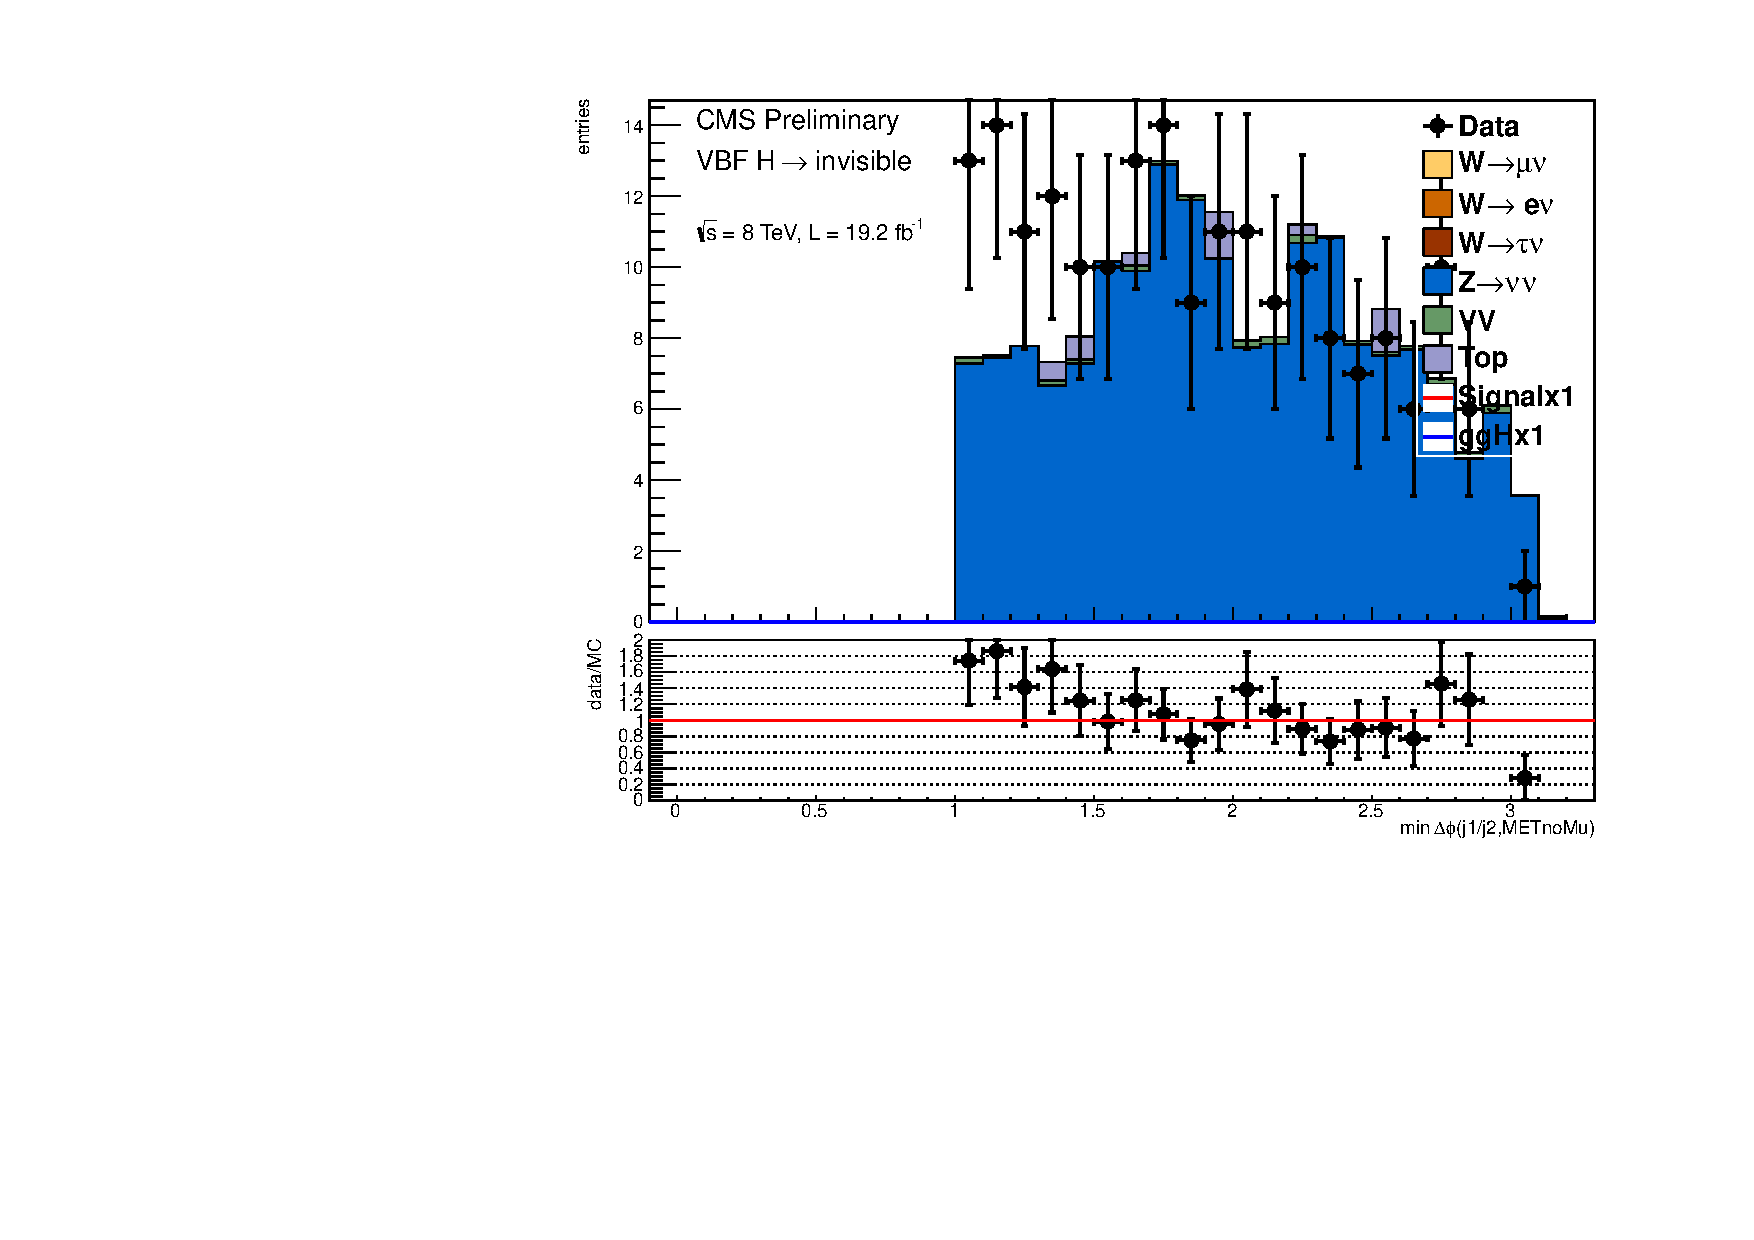
\includegraphics[width=.5\textwidth]{../../Thesis/plots/parked/HIG-14-038-figs/output_sigreg/mumu_jetmetnomu_mindphi.pdf}
    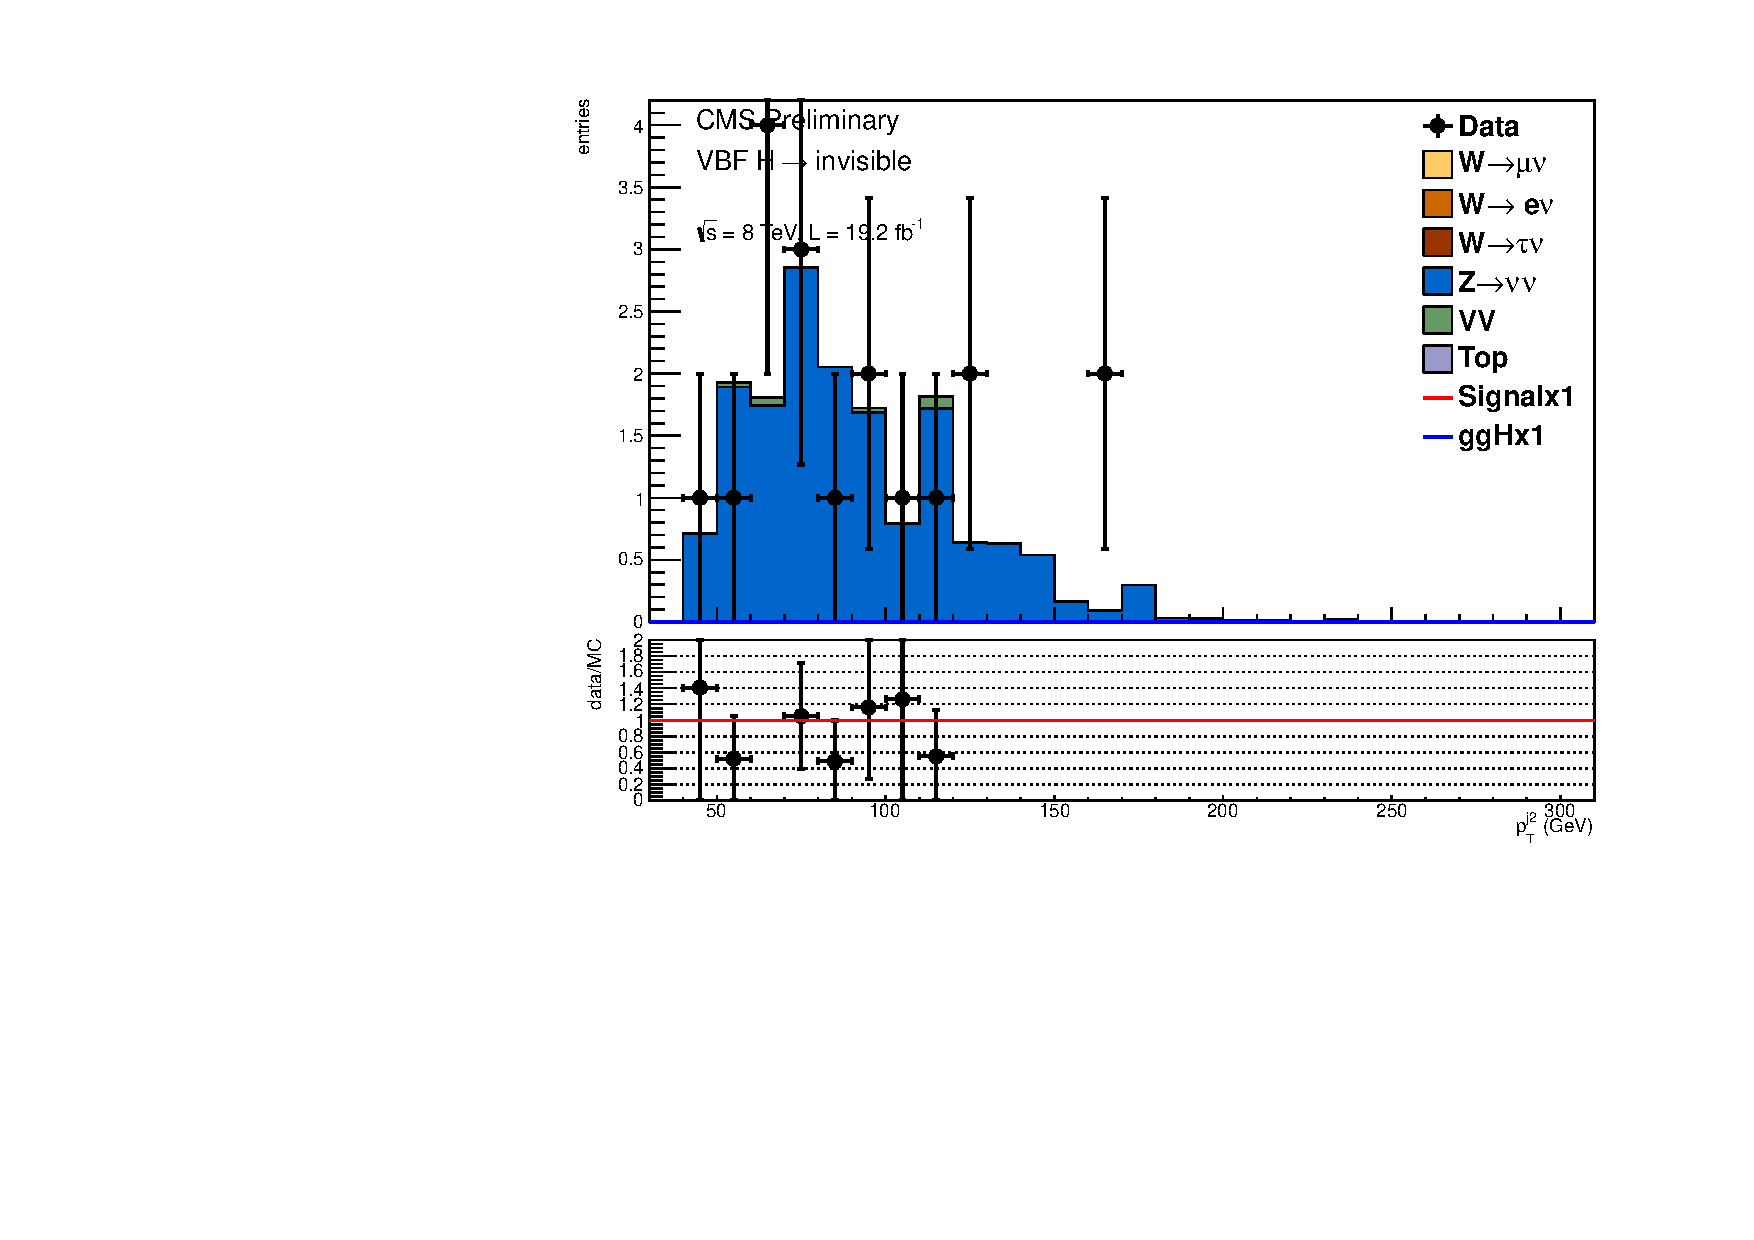
\includegraphics[width=.5\textwidth]{../../Thesis/plots/parked/HIG-14-038-figs/output_sigreg/mumu_jet2_pt.pdf}
  \end{frame}



  %Remaining background estimation QCD, how it evolved
  \begin{frame}
    \frametitle{QCD Estimation}
    \begin{block}{}
      \begin{itemize}
      \item Small phase space between trigger thresholds and signal region
      \item Invert QCD reduction criteria to obtain a shape for QCD background
      \item Normalised using fit of scale factor in sideband 1 as QCD reduction criteria are tightened
      \end{itemize}
    \end{block}
    \begin{columns}
      \column{.5\textwidth}
      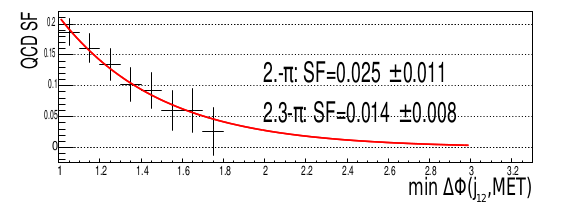
\includegraphics[width=\textwidth]{TalkPics/RHULSeminar051016/qcdfit.png}

      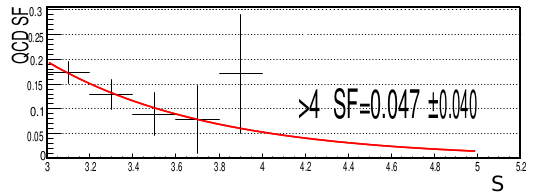
\includegraphics[width=\textwidth]{TalkPics/RHULSeminar051016/qcdfit2.png}
      \column{.5\textwidth}
      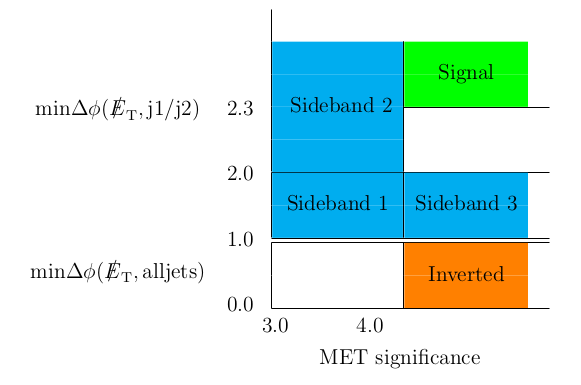
\includegraphics[width=\textwidth]{TalkPics/RHULSeminar051016/qcddiag.png}
    \end{columns}
  \end{frame}

  %Selection: selection optimisation
  \begin{frame}
    \frametitle{Selection Optimisation}
    \begin{block}{}
      \begin{itemize}
      \item Final selection was determined by tightening preselection requirements to find optimum expected limit
      \item Selection driven by the preselection and limited numbers of events in background control regions
      \end{itemize}
    \end{block}
    \begin{columns}
      \column{.5\textwidth}
      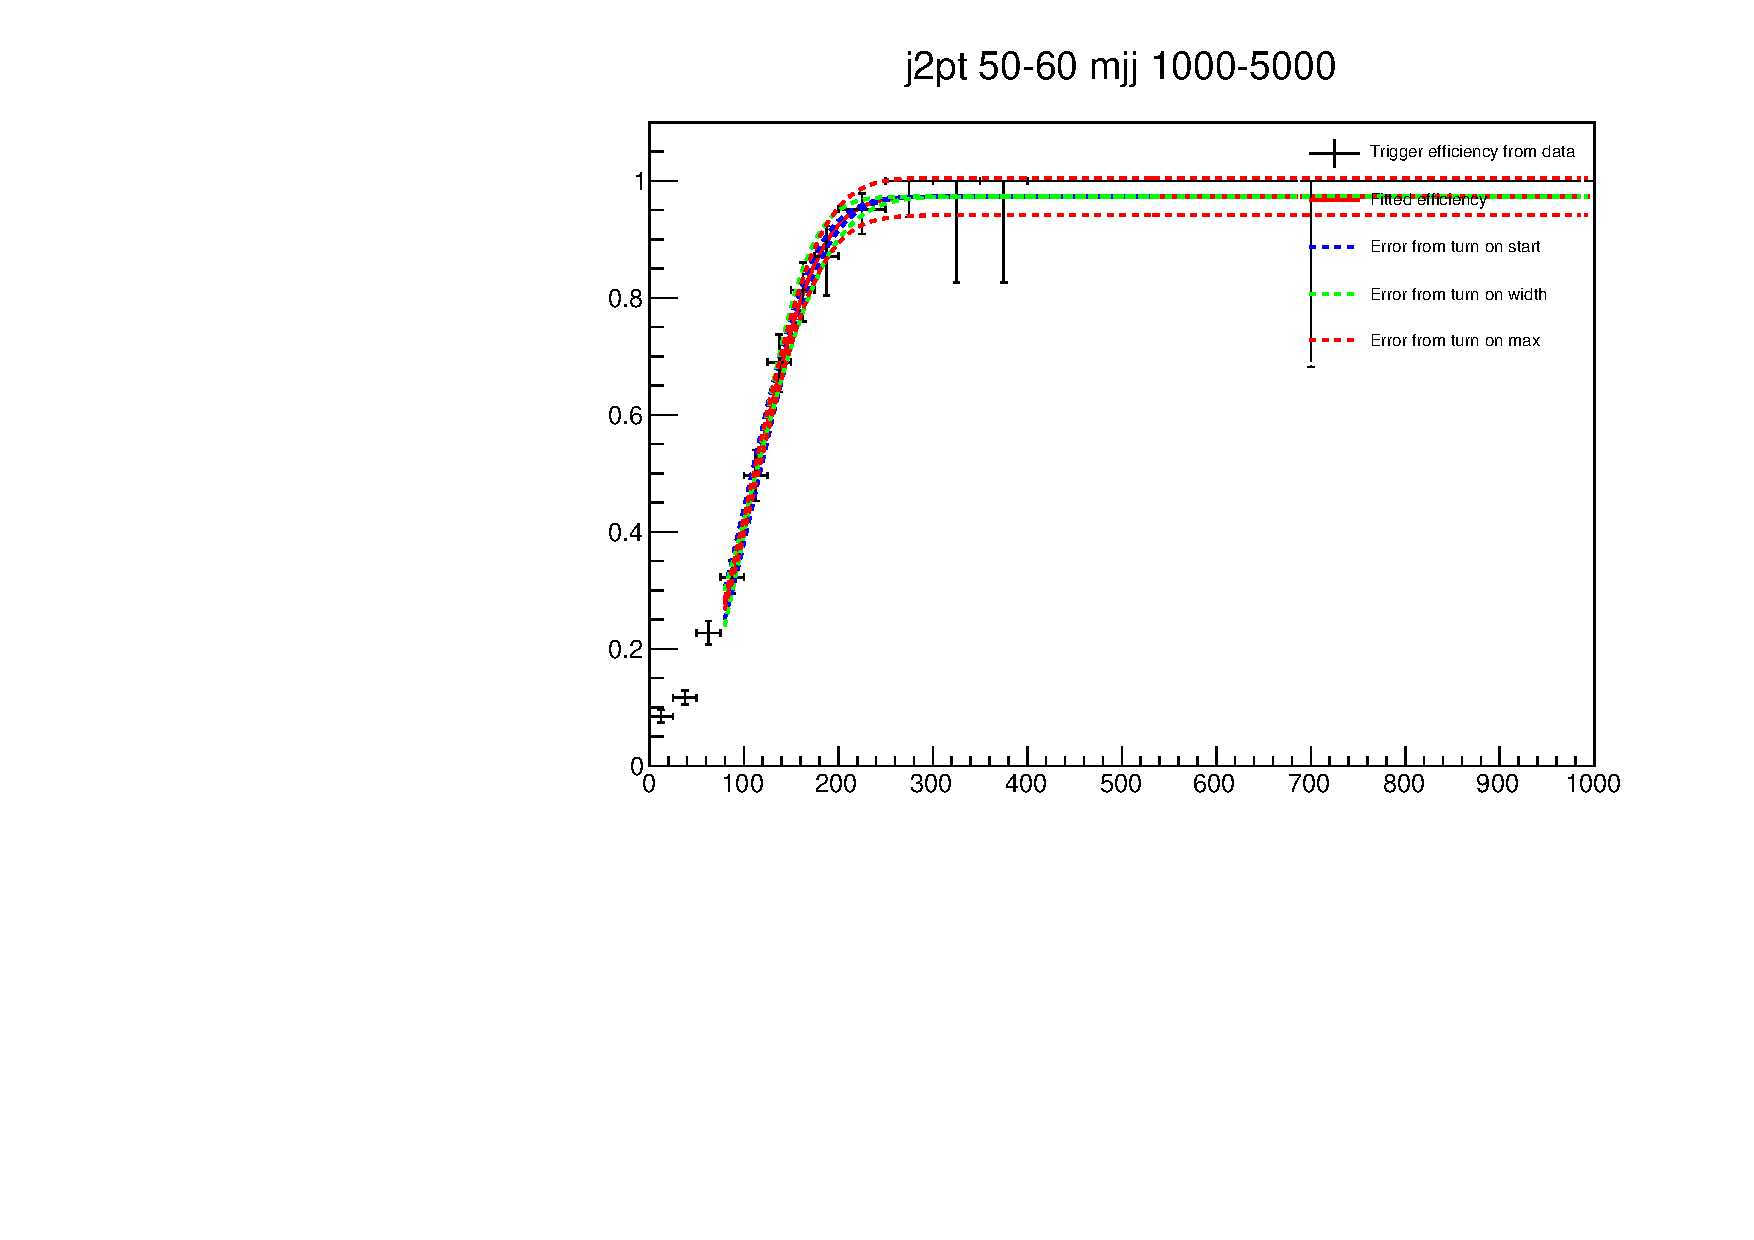
\includegraphics[width=\textwidth]{../../Thesis/plots/parked/AN-14-243-figs/trigfitplots/hData_MET_1D_35D.pdf}
      \column{.55\textwidth}
      \vspace{-.2cm}
      \begin{block}{}
        \scriptsize
        \begin{tabular}{l|c}
          Variable & Requirement \\
          \hline
          $\eta_{j1}.\eta_{j2}$ &$<0$ \\
          jet 1 $p_{T}$ & $>50$ GeV \\
          jet 2 $p_{T}$ & $>45$ GeV \\
          $\Delta\eta_{jj}$ & $>3.6$ \\
          $M_{jj}$ & $>1200$ GeV \\
          $E_{T}^{miss}$ & $>90$ GeV \\
          $E_{T}^{miss}$ significance & $>4$ GeV \\
          min$\Delta\phi$(j,$E_{T}^{miss}$)&$>2.3$ \\
        \end{tabular}
      \end{block}
      \end{columns}
  \end{frame}

  \begin{frame}
    \frametitle{Systematic uncertainties}
    \begin{block}{}
      \scriptsize
      \begin{tabular}{lcc}
        \hline \hline
        Source  & Total background & Signal     \\
        \hline
        Control region statistics & 9.3 & - \\
        MC statistics & 5.4 & 3.8 \\
        JES & 4.6 & 11 \\
        $W\rightarrow\tau\nu$ control region extrapolation & 4.3 & - \\
        QCD background estimation & 3.2 & - \\
        JER & 3.0 & 1.8 \\
        Lepton ID efficiency & 2.4 & - \\
        UES & 1.9 & 1.6 \\
        Pileup weight & 1.1 & 1.5 \\
        Top MC scale factor unc. & 0.25 & - \\
        Luminosity & 0.02 & 2.6 \\
        QCD scale, PDF and cross-section uncertainties & 0.01 & 5.2 \\
        \hline
        Total & 13.6 & 13.3 \\
        \hline \hline
      \end{tabular}
    \end{block}
  \end{frame}



  \begin{frame}
    \frametitle{What did we see?}
    \begin{block}{}
      \centering
      \begin{tabular}{lc}
        \hline \hline
        Process & Event yields \\
        \hline
        $Z\rightarrow\nu\nu$&$158.1 \pm 37.3 \pm 21.2$\\
        $W\rightarrow e\nu$&$57.9 \pm 7.4 \pm 7.7$\\
        $W\rightarrow\mu\nu$&$102.5 \pm 6.2 \pm 11.7$\\
        $W\rightarrow\tau\nu$&$94.6 \pm 13.1 \pm 23.8$\\
        top&$5.5 \pm  1.8$\\
        Minor backgrounds&$3.9 \pm 0.7$\\
        QCD multijet &$17\pm 14$\\
        \hline
        Total background &$439.4 \pm 40.7 \pm 43.5 $\\
        \hline
        Signal(VBF) &$273.1 \pm 31.2 $\\
        Signal(ggH) &$23.1 \pm 15.9 $\\
        \hline
        Observed data & 508 \\
        \hline \hline
      \end{tabular}
      \begin{itemize}
      \item Small 1 $\sigma$ excess seen
      \end{itemize}
    \end{block}
  \end{frame}

  \begin{frame}
    \frametitle{Control plots}
    \centering
    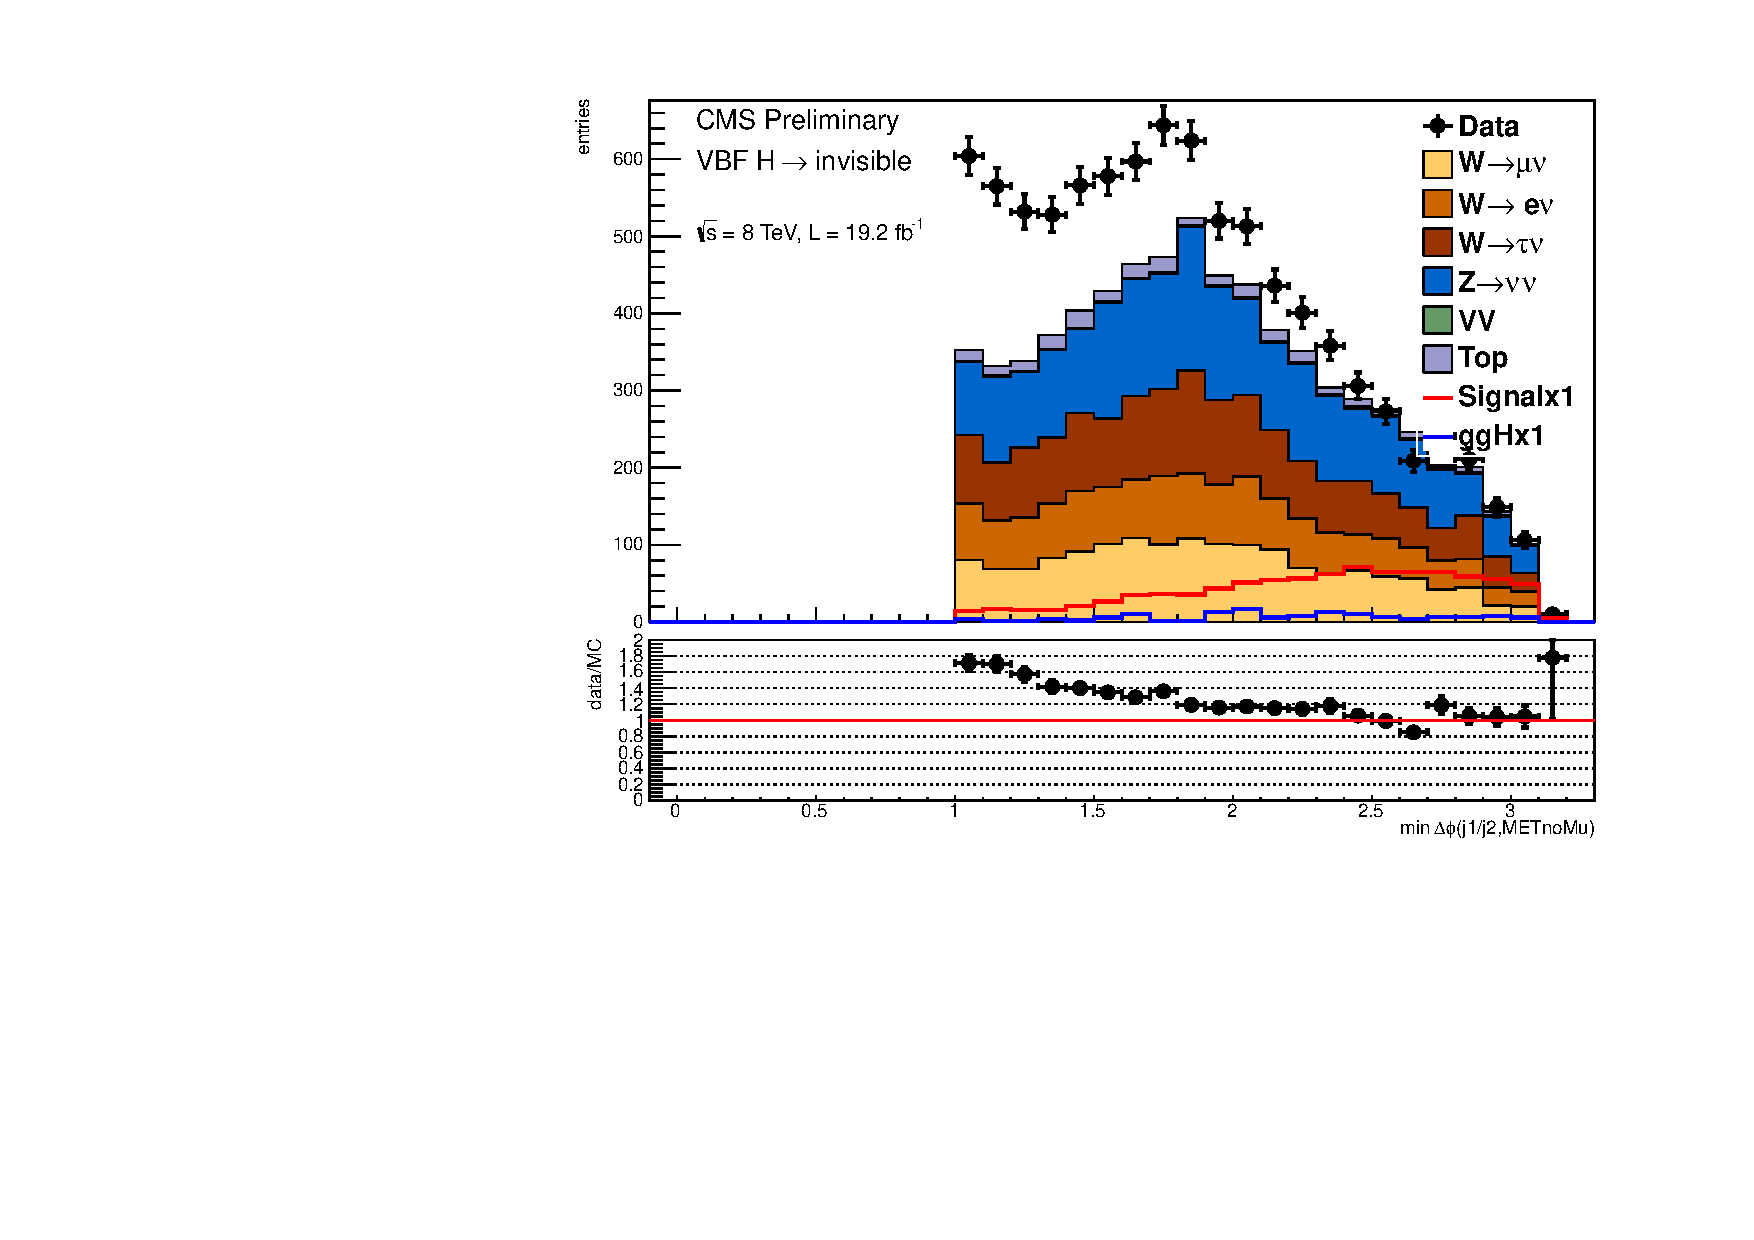
\includegraphics[width=.45\textwidth]{../../Thesis/plots/parked/HIG-14-038-figs/output_sigreg/nunu_jetmetnomu_mindphi.pdf}
    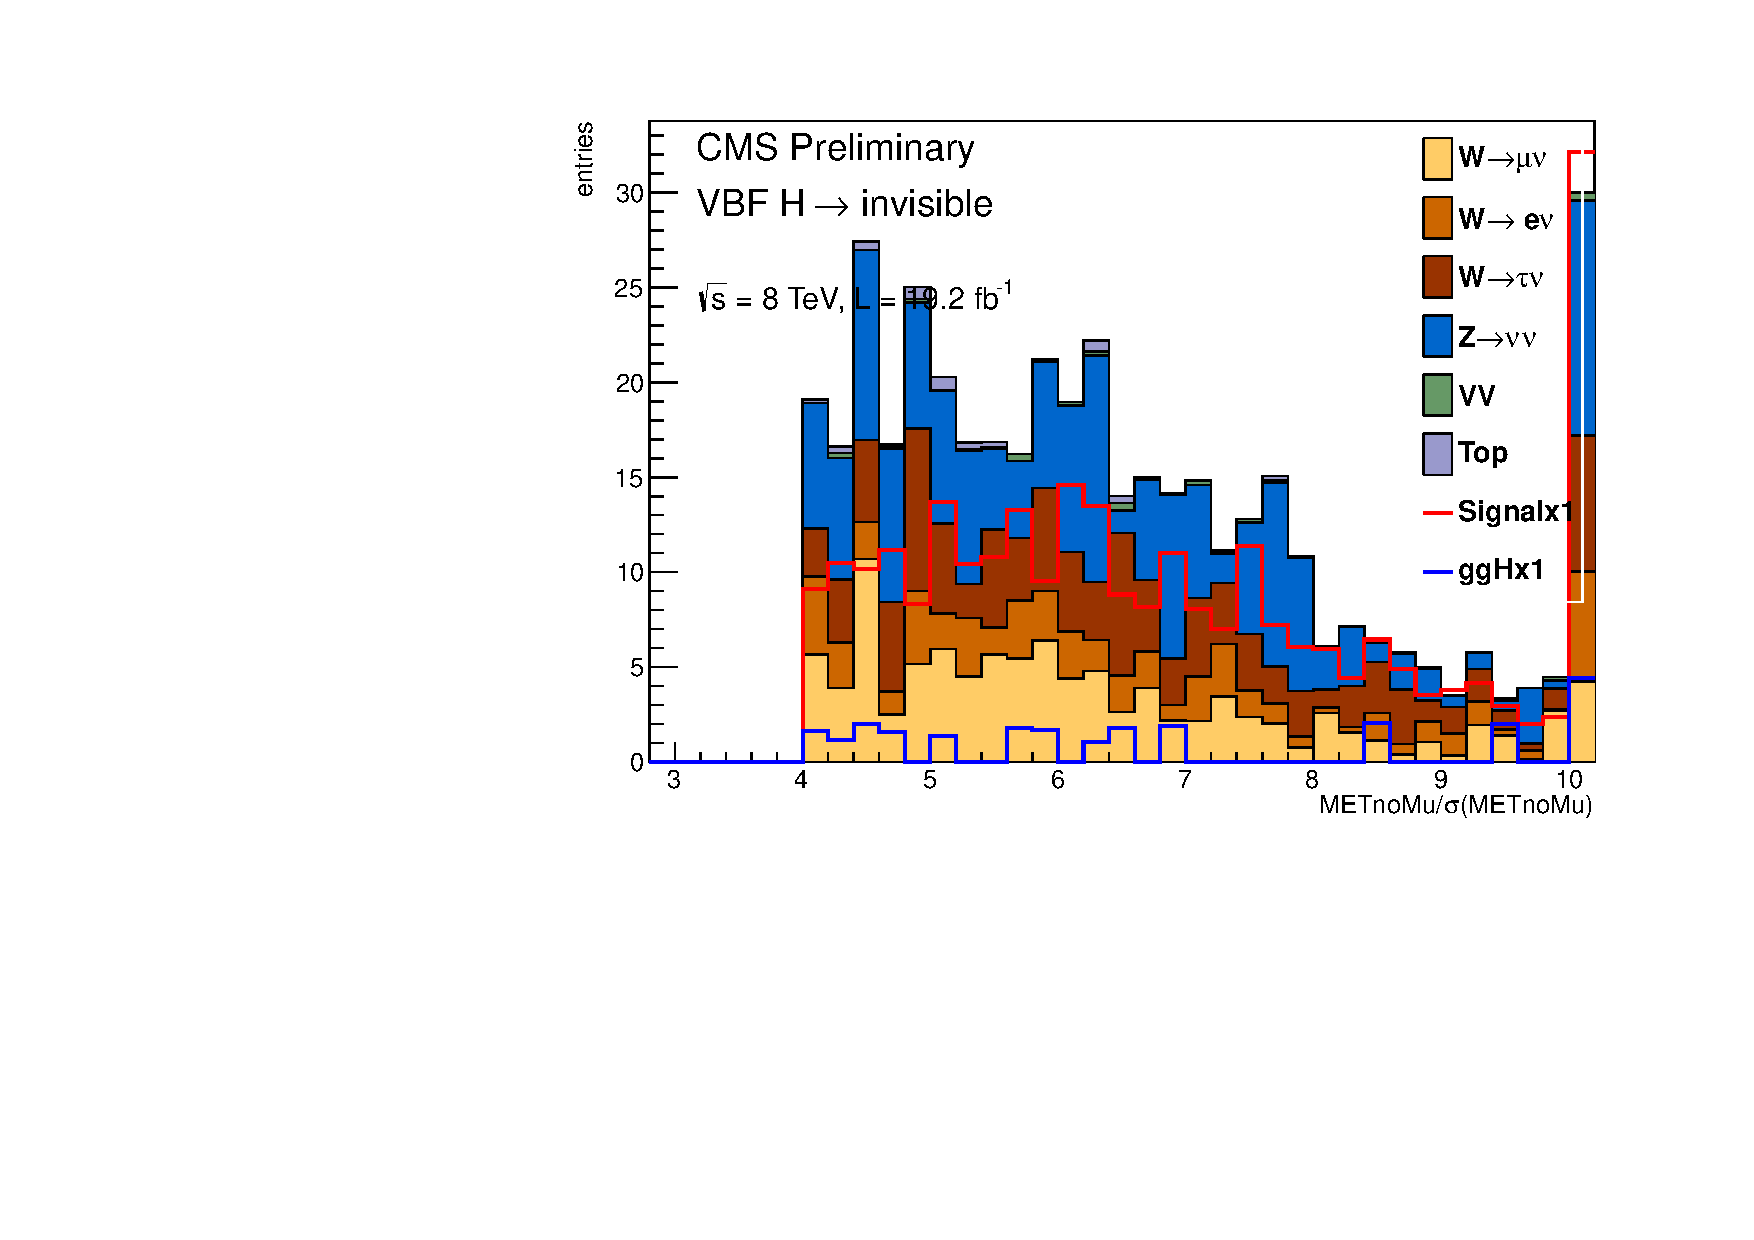
\includegraphics[width=.45\textwidth]{../../Thesis/plots/parked/HIG-14-038-figs/output_sigreg/nunu_metnomu_significance.pdf}

    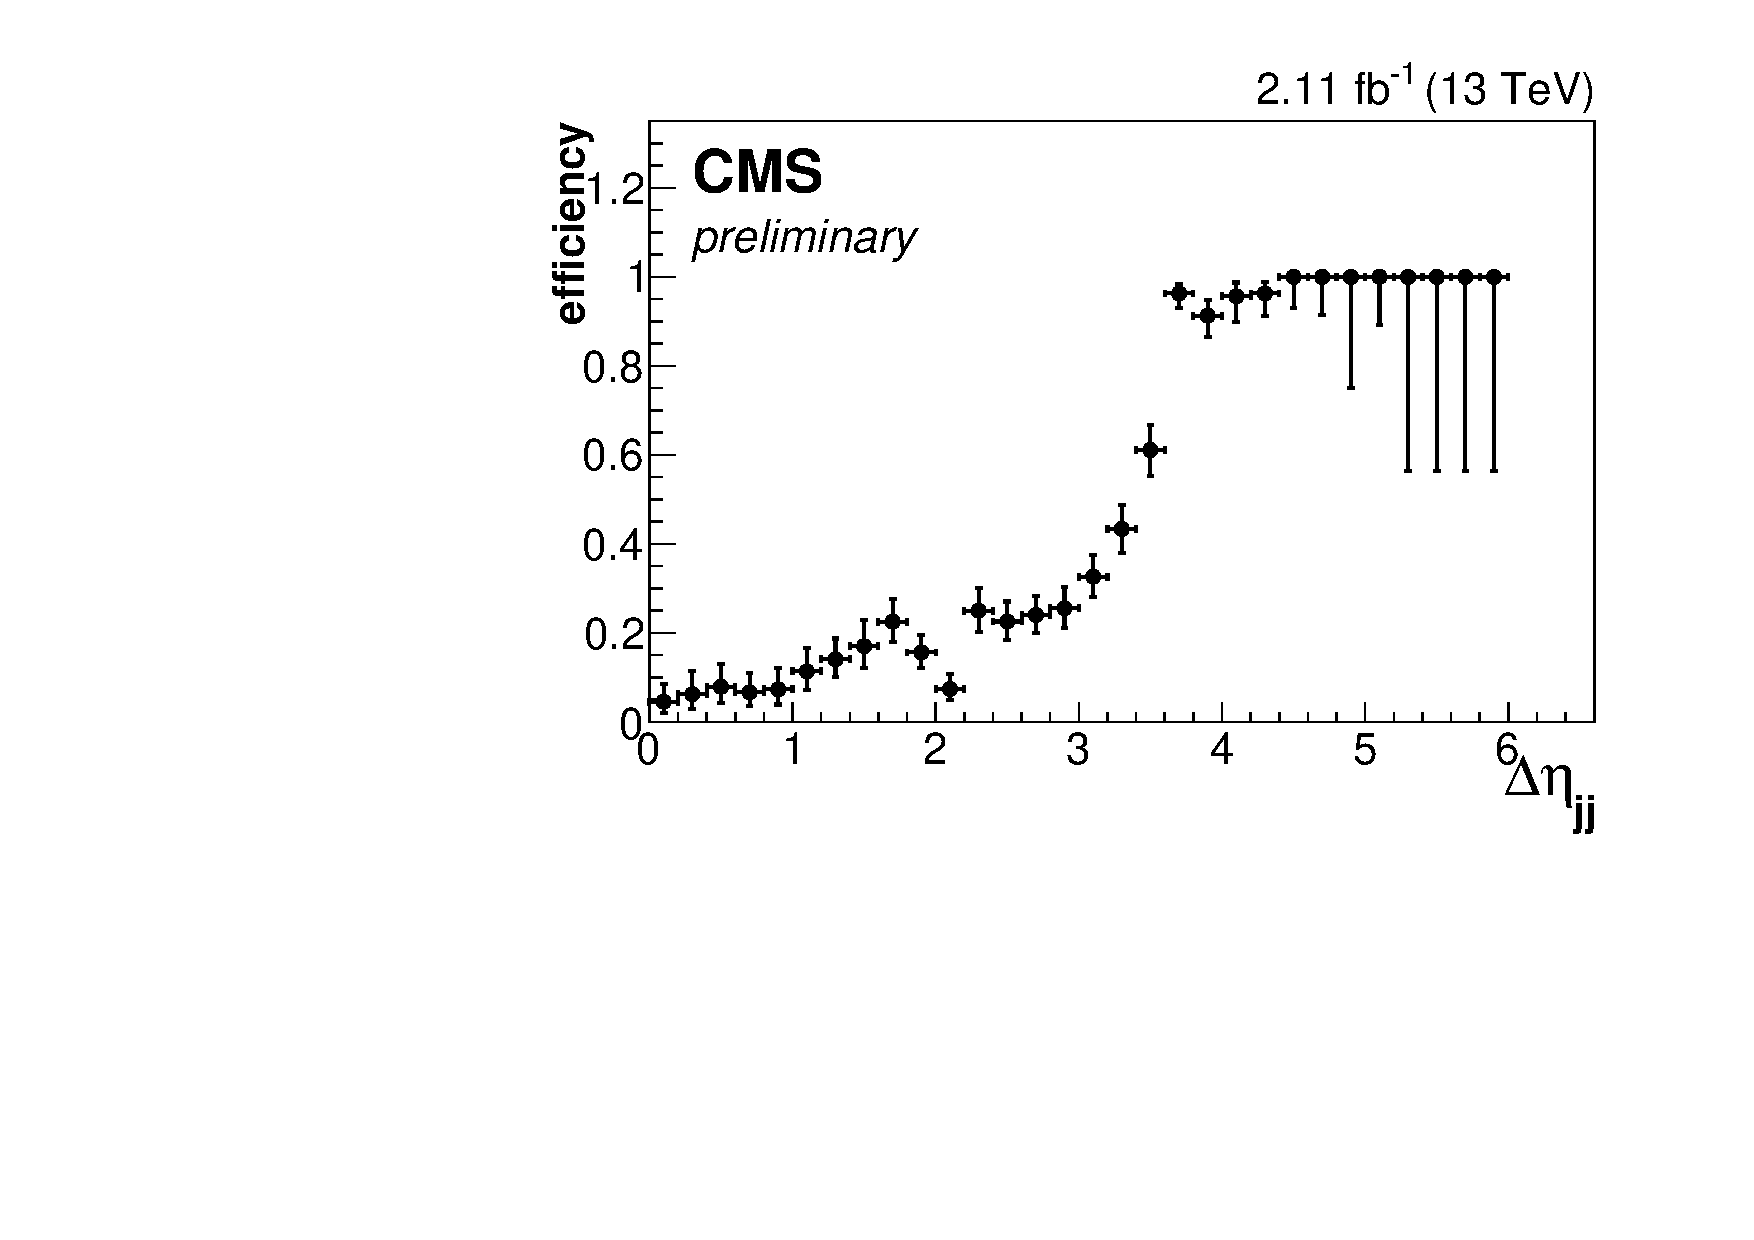
\includegraphics[width=.45\textwidth]{../../Thesis/plots/parked/HIG-14-038-figs/output_sigreg/nunu_dijet_deta.pdf}
    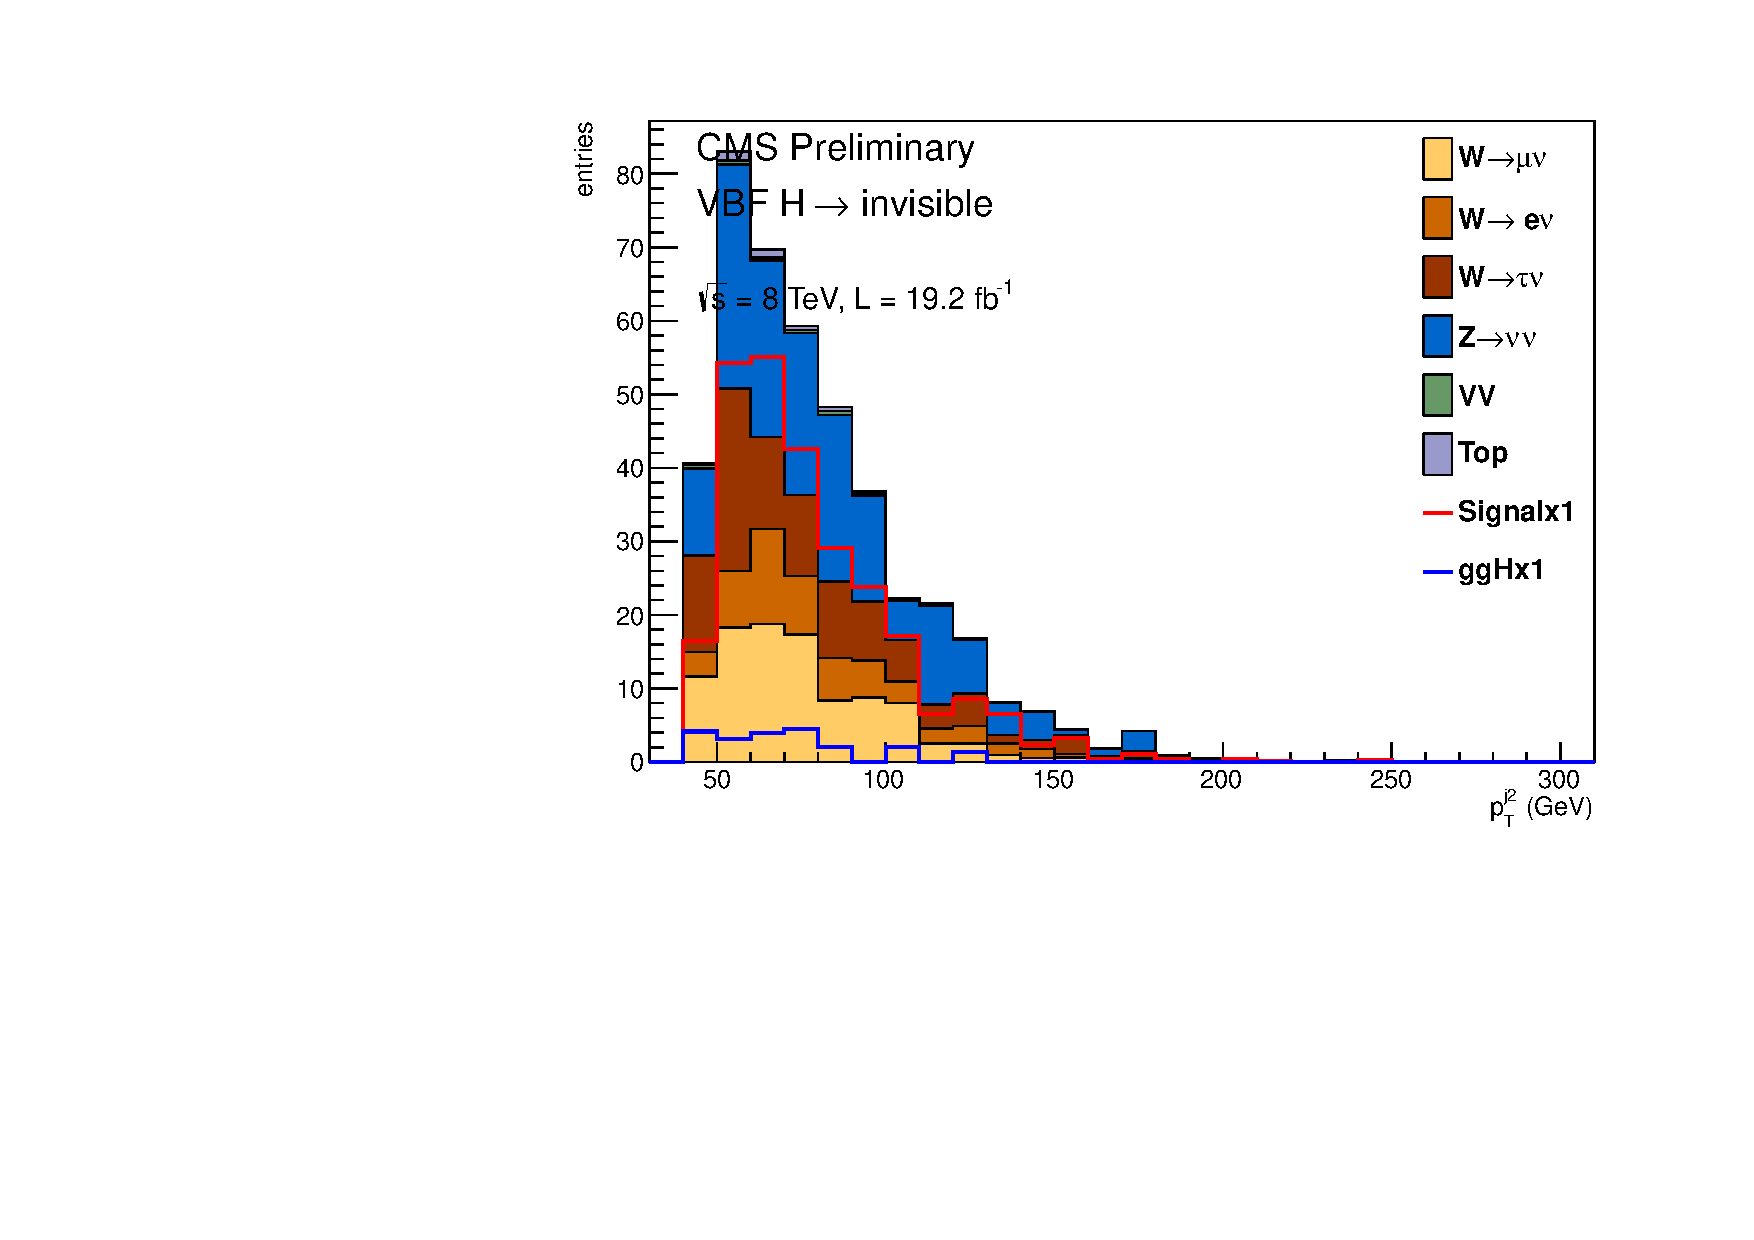
\includegraphics[width=.45\textwidth]{../../Thesis/plots/parked/HIG-14-038-figs/output_sigreg/nunu_jet2_pt.pdf}
  \end{frame}

  \begin{frame}
    %HIG-14-038
    \frametitle{Limits from Run 1 VBF search}%parked
    \begin{columns}
      %quick description of parked data  
      \column{.5\textwidth}
      \vspace{-.3cm}
      \begin{block}{}
        \small
        \vspace{-.2cm}
        \begin{itemize}
        \item Perform a single bin counting experiment using LHC $CL_{S}$ formalism
        \item 95\% CL Observed (expected) limit on $\mathcal{B}\left(H\rightarrow inv.\right)$ for $m_{H}=$125 GeV is 57 (40)\%
        \item All V+jets normalisations were allowed to float separately
        \item[-] If all V+jets normalisations had same uncertainty as $W\rightarrow\mu\nu$ expected limit would be 33\%
        \end{itemize}
      \end{block}
      \column{.5\textwidth}
      %limit plot from hig-14-038
      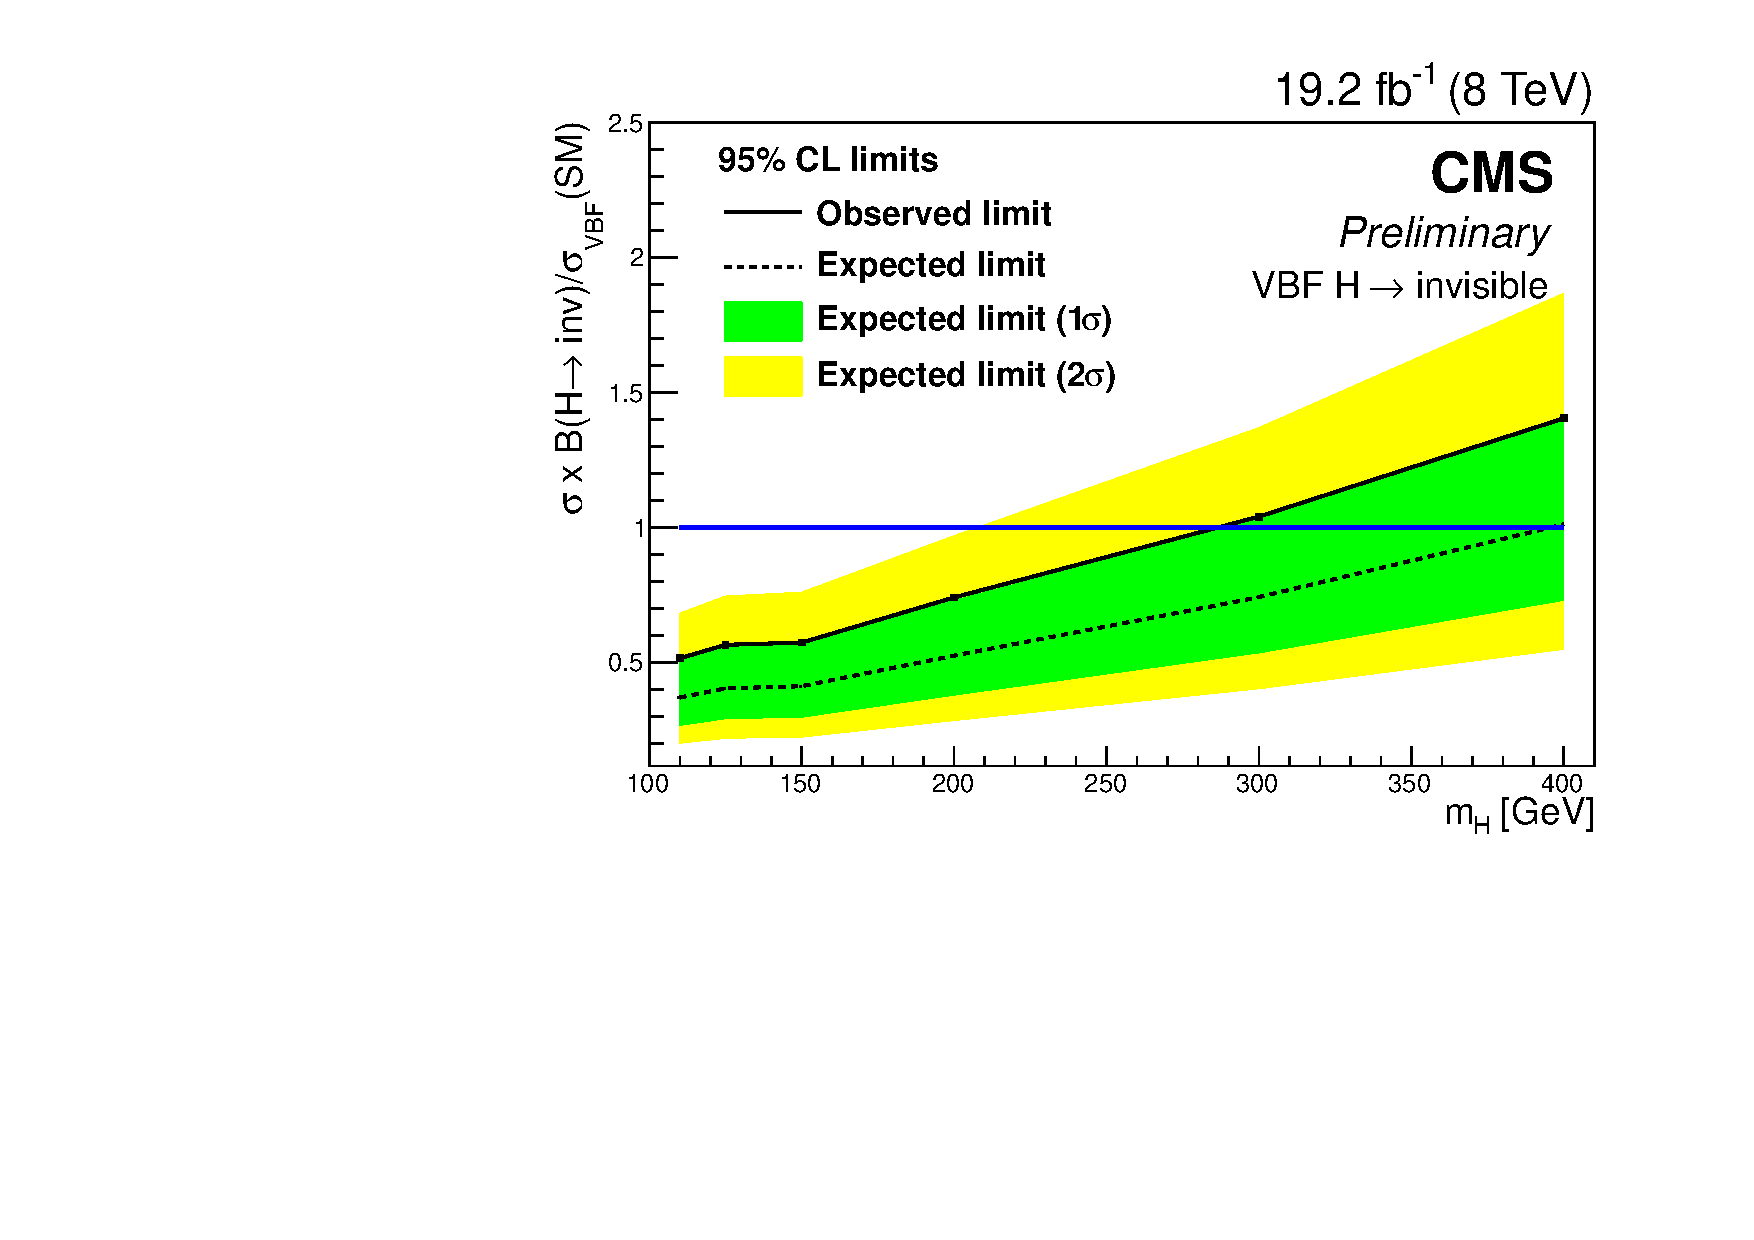
\includegraphics[width=\textwidth]{TalkPics/DM@LHC2016/Figure_007-a.pdf}
      \centering
      \scriptsize
      
      CMS-PAS-HIG-14-038
    \end{columns}
  \end{frame}


  %intro to ZH searches
  \begin{frame}
    \centering
    \huge\textcolor{beamer@icmiddleblue}{Other Run 1 analyses}
  \end{frame}

  %CMS Run 1
  \begin{frame}
    %HIG-13-030
    \frametitle{Run 1 CMS direct searches - ZH}
    \begin{columns}
      %quick description comb from hig-13-030
      \column{.5\textwidth}
      \begin{block}{}
        \small
        \begin{itemize}
        \item Searches in $Z\rightarrow\ell\ell$ and $Z\rightarrow b\bar{b}$ channels
        \item $Z(\ell\ell)H$ search is a 2D shape analysis with data driven backgrounds
        \item $Z(b\bar{b})H$ search is a BDT shape analysis with data driven backgrounds
        \item Combined $ZH$ searches observed (expected) limit on $\mathcal{B}\left(H\rightarrow inv.\right)$ for $m_{H}=$125 GeV is 81 (83)\%
        \end{itemize}
      \end{block}
      \column{.5\textwidth}
      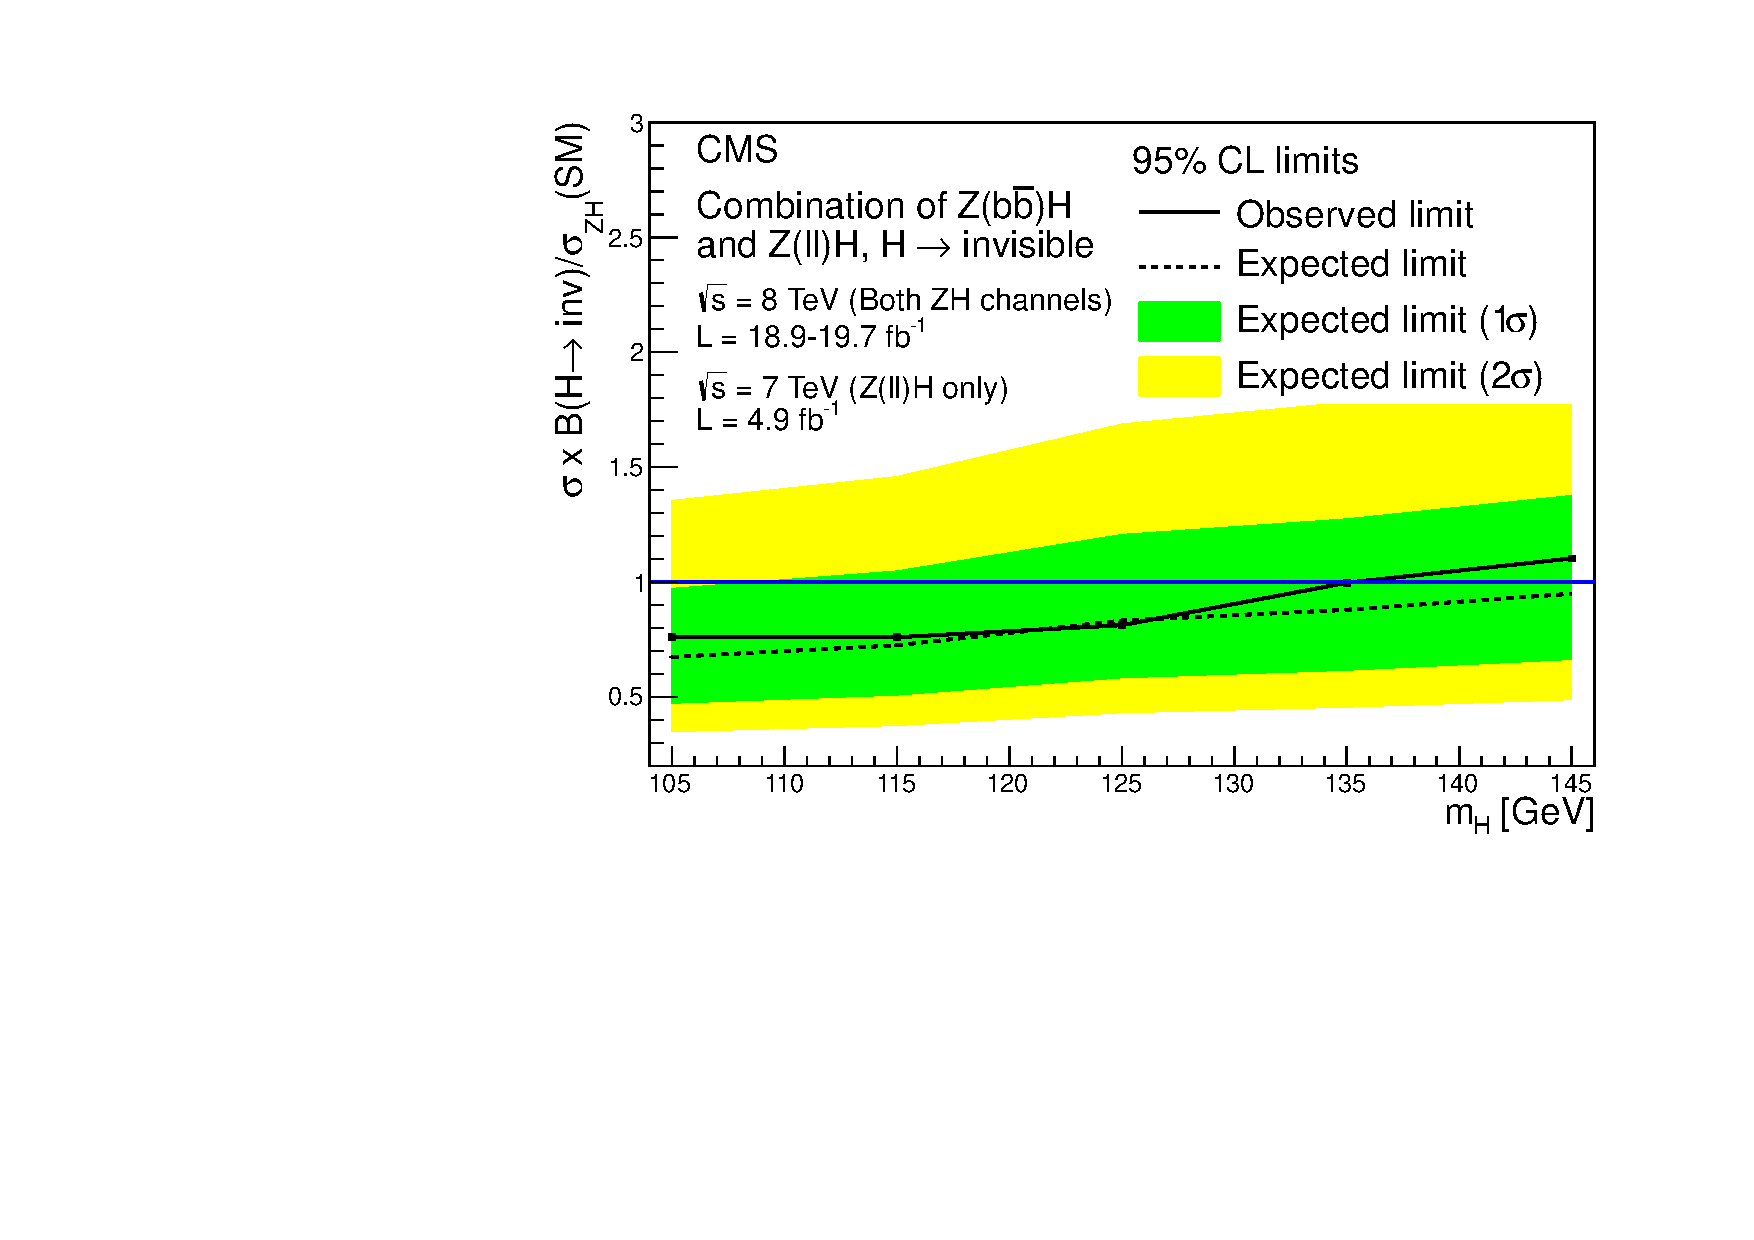
\includegraphics[width=\textwidth]{TalkPics/DM@LHC2016/Fig9b-ZH-LimitNorm.pdf}      
      \centering
      \scriptsize
      
      Eur. Phys. J. C 74 (2014) 2980
    \end{columns}
  \end{frame}

  \begin{frame}
    %EXO-12-055
    \frametitle{Run 1 CMS direct searches - Monojet+V(had)H}
    \begin{columns}
      %quick description
      \column{.5\textwidth}
      \begin{block}{}
        \small
        \begin{itemize}
        \item Search has categories targeting $V(had)H$ and $ggH$ production modes
        \item $E_{T}^{miss}$ shape analysis with data driven background estimation
        \item Observed (expected) limit on $\mathcal{B}\left(H\rightarrow inv.\right)$ for $m_{H}=$125 GeV is 53 (62)\%
        \end{itemize}
      \end{block}
      \column{.5\textwidth}
      %fig 8b from pas
      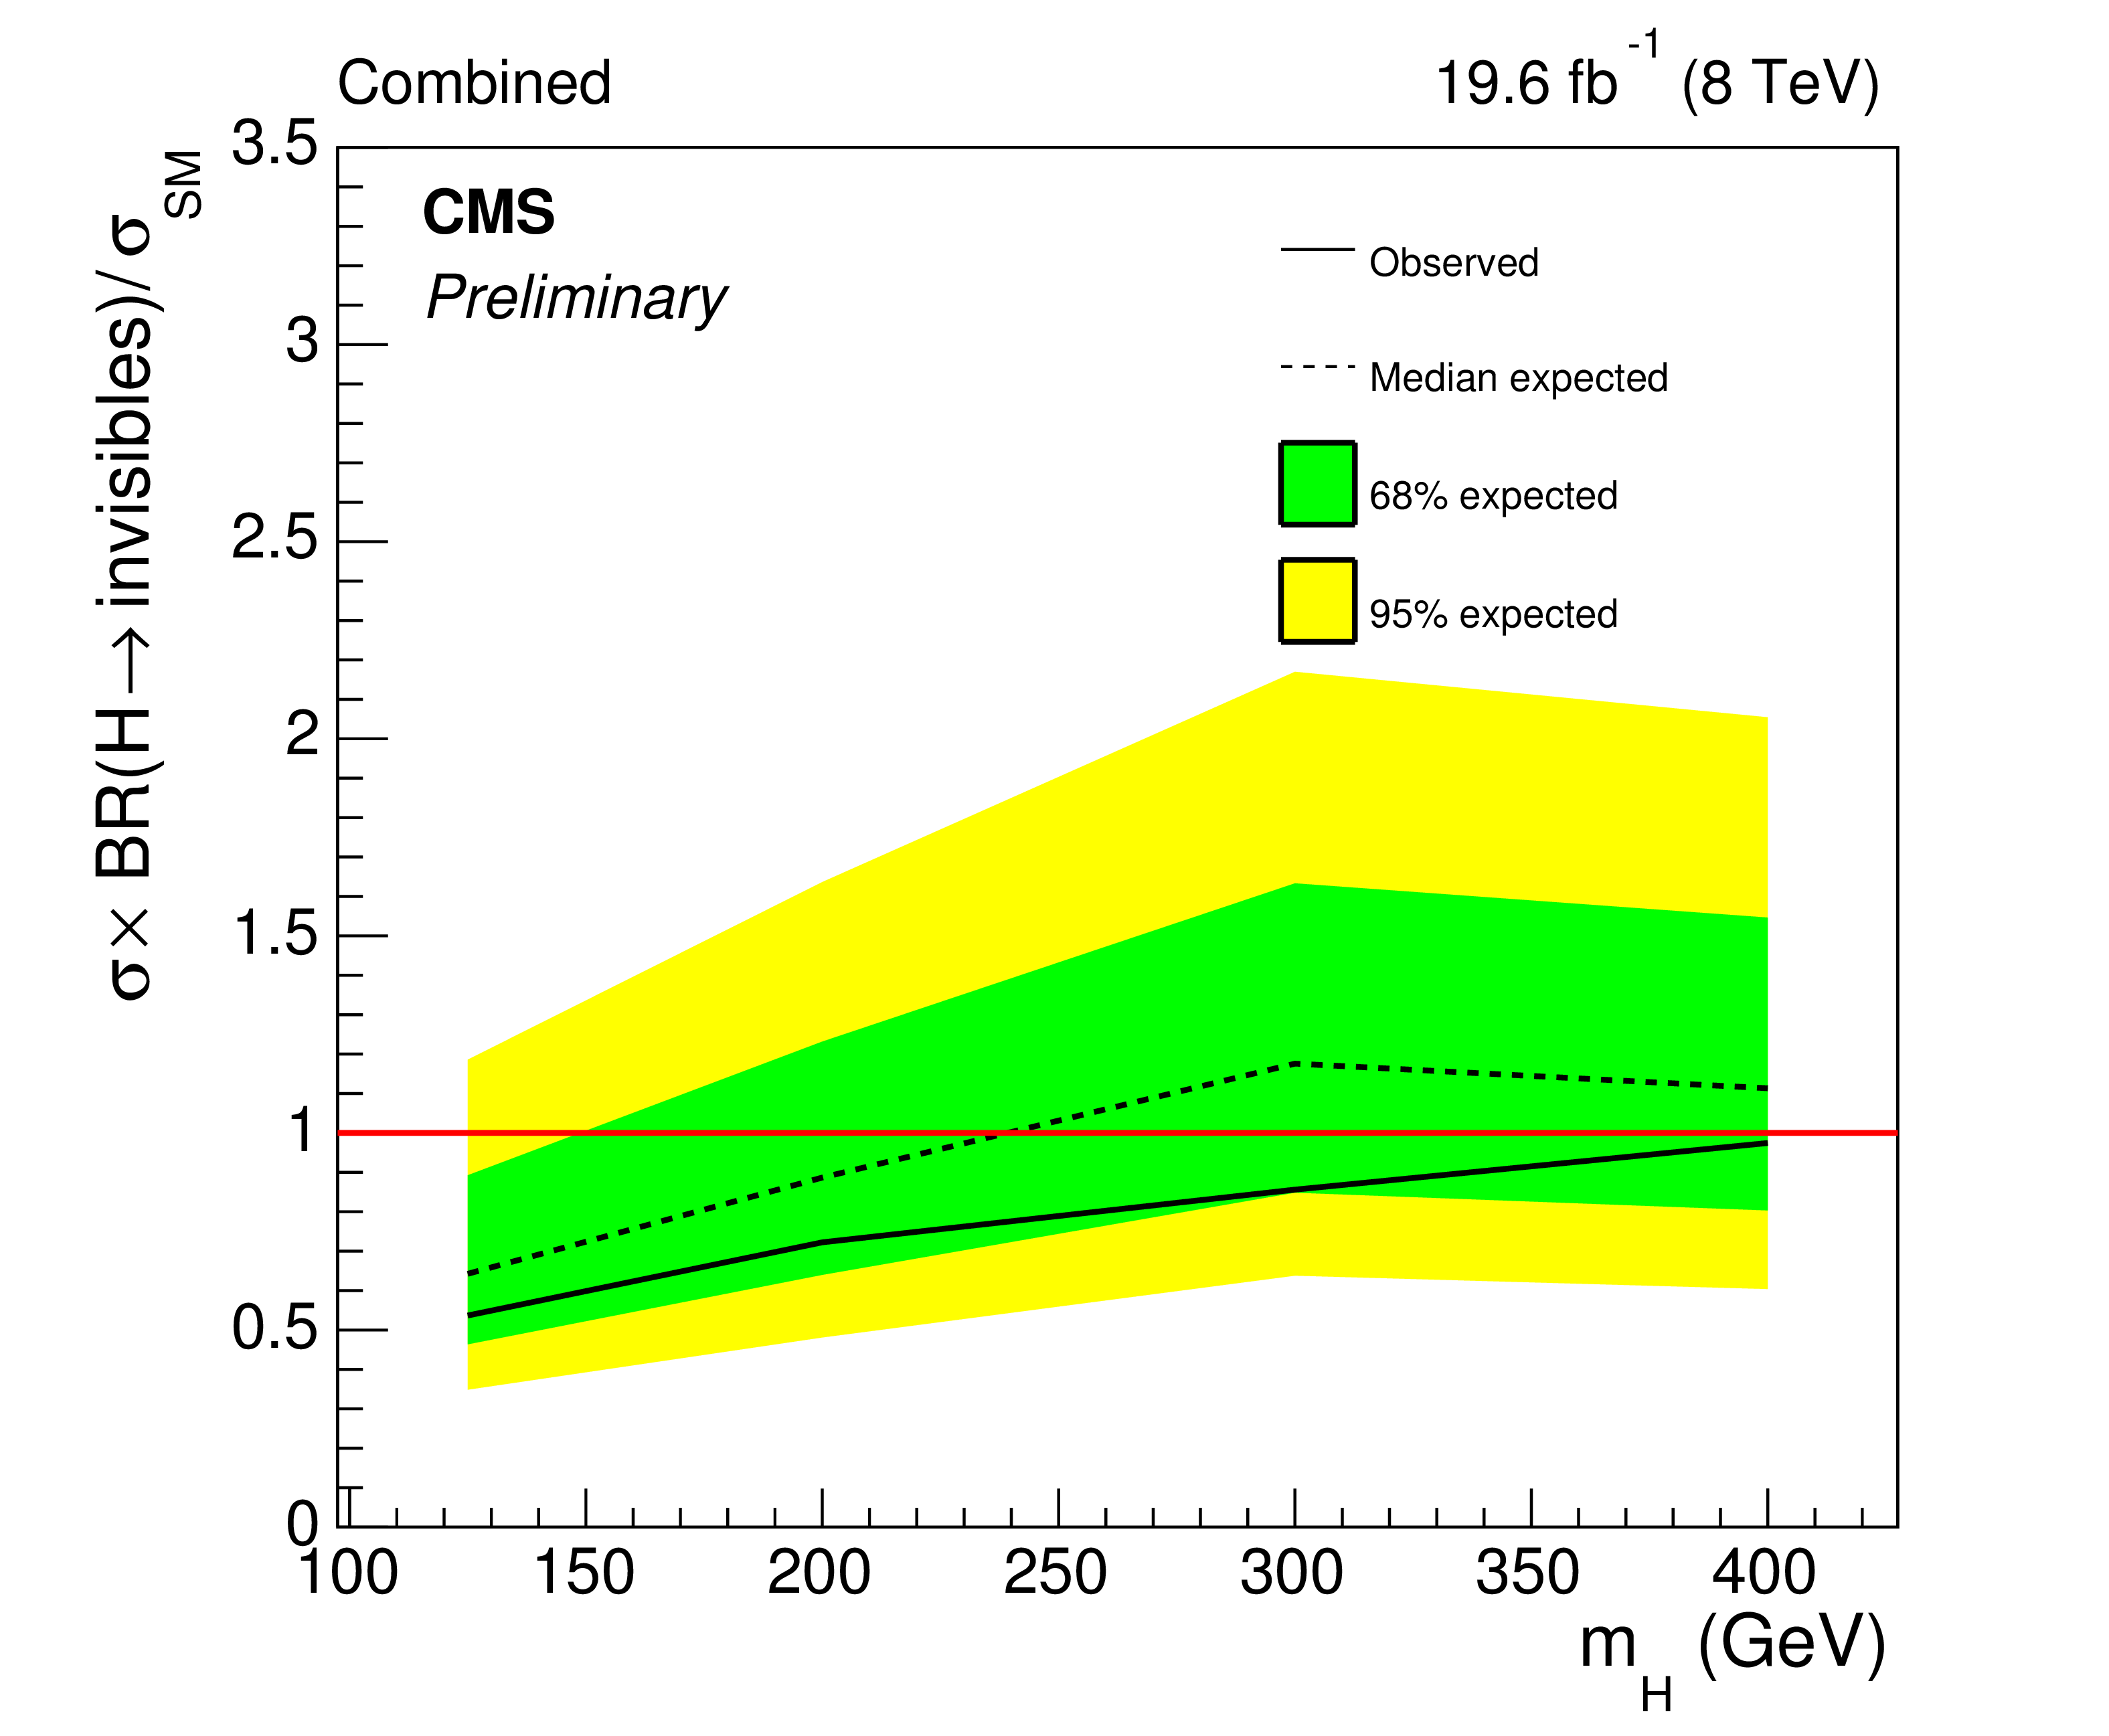
\includegraphics[width=\textwidth]{TalkPics/DM@LHC2016/CMS-PAS-EXO-12-055_Figure_008-b.png}
      \centering
      \scriptsize
      
      CMS-PAS-EXO-12-055
    \end{columns}
  \end{frame}

  %why combine and how does CMS handle correlated errors
  \begin{frame}
    \frametitle{Combining}
    \begin{block}{}
      \begin{itemize}
      \item Best result can be obtained by combining all available searches
      \item Must properly account for correlations between channels
      \item[-] CMS framework only allows for 100\% or 0\% correlation of a parameter
      \item Most energy resolutions and reconstruction efficiencies are centrally calculated so the uncertainties on these are correlated
      \item Exceptions are jet uncertainties in monojet analysis which are not correlated due to very different kinematics from other analyses
      \item Some cross-section uncertainties are also correlated between channels
      \end{itemize}
    \end{block}
  \end{frame}

  %Combinations expand
  \begin{frame}
    %HIG-15-012
    \frametitle{Run 1 CMS direct searches - Combination}
    \vspace{-.2cm}
    \begin{block}{}
      \small
      \begin{itemize}
        \vspace{-.1cm}
      \item Combine by production mode as well as full combination
        \vspace{-.2cm}
      \item[-] ggH-tagged is monojet, VH-tagged is Z($\ell\ell$)H+Z($bb$)H+V(had)H, VBF-tagged is VBF
      \item Obs. (exp.) limit on $\mathcal{B}\left(H\rightarrow inv.\right)$ at $m_{H}=$125 GeV was 36 (30)\%
      \end{itemize}
    \end{block}
    \begin{columns}
      %by category plot
      \column{.5\textwidth}
      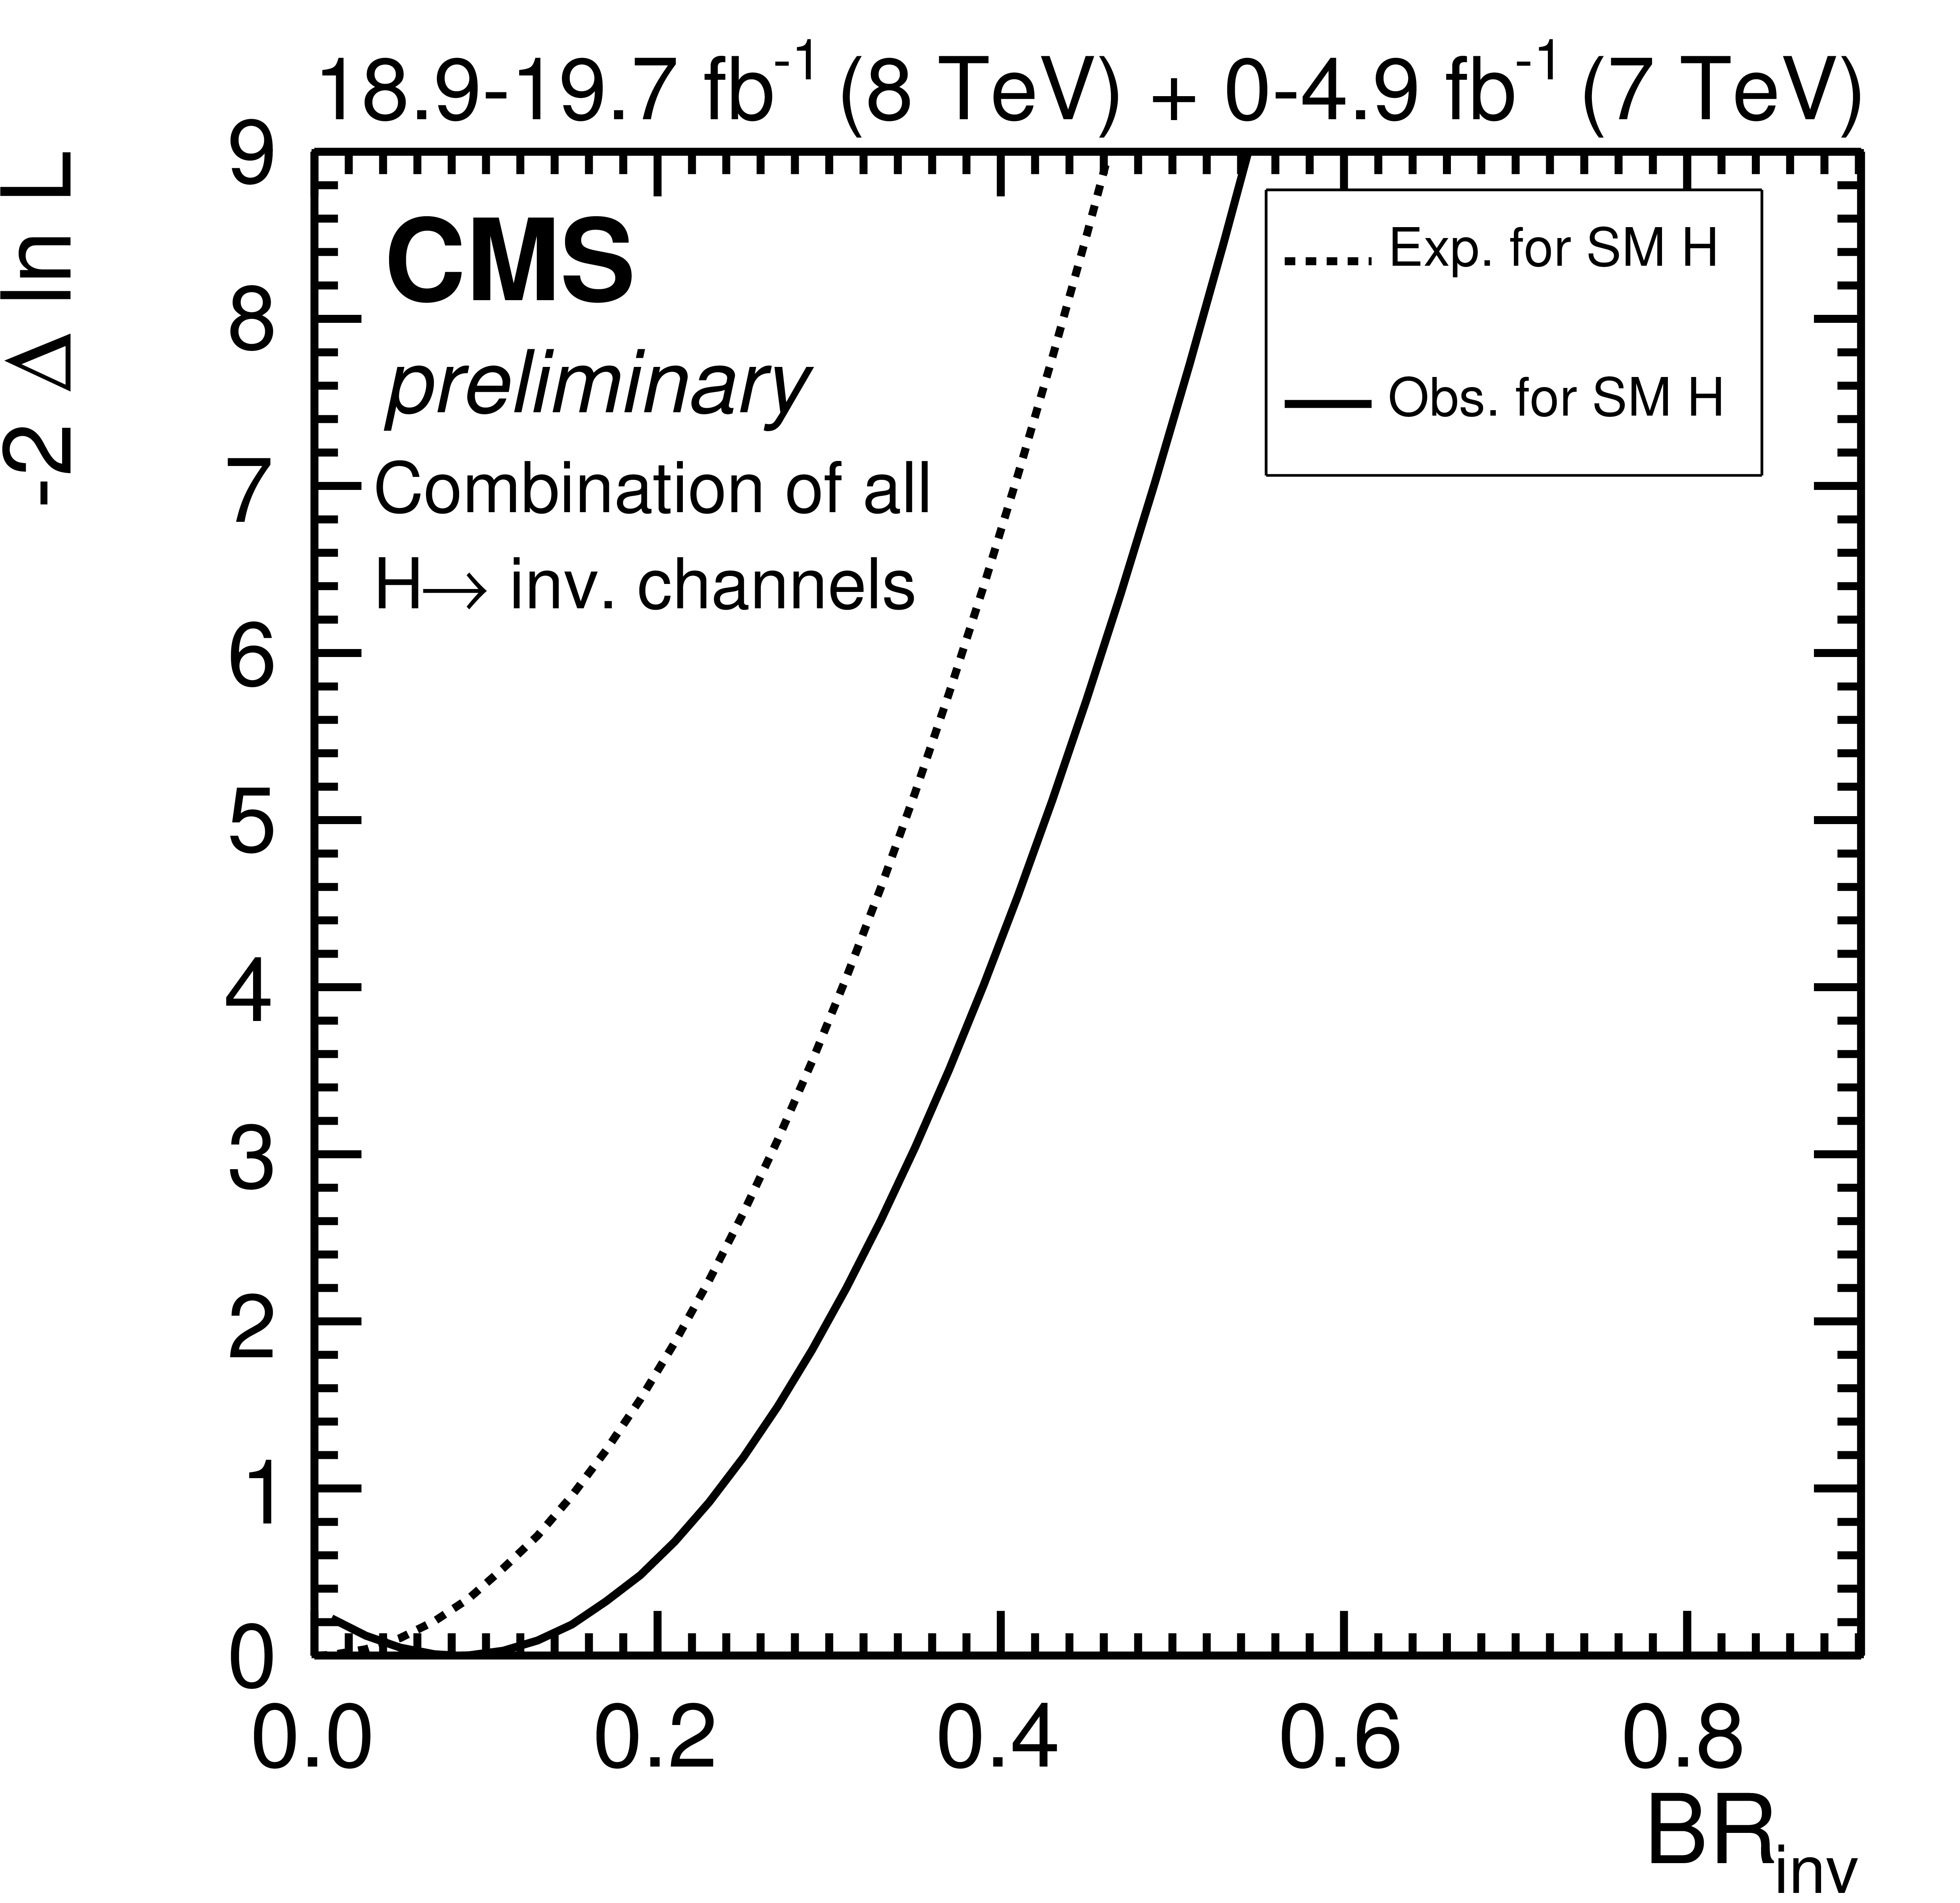
\includegraphics[width=.8\textwidth]{TalkPics/DM@LHC2016/CMS-PAS-HIG-15-012_Figure_002.png}
      \column{.5\textwidth}
      \includegraphics[width=.9\textwidth]{TalkPics/DM@LHC2016/CMS-PAS-HIG-15-012_Figure_003.png}
    \end{columns}
    \centering
    \scriptsize
    
    CMS-PAS-HIG-15-012
  \end{frame}

  \begin{frame}
    \centering
    \huge\textcolor{beamer@icmiddleblue}{Run 2}
  \end{frame}

  %Moving to a simultaneous fit for run 2
  \begin{frame}
    \frametitle{Run 2 CMS direct searches - VBF improvements}
    \begin{block}{}
      \begin{itemize}
      \item Dominant uncertainty in Run 1 was control region statistics
      \item In order to improve this all W+jets processes now assumed to share the same scale factor
      \item[-] True in the absence of mismodelling of lepton identification efficiency
      \item[-] Previous results show compatible scale factors within statistical errors
      \item W+jets and Z+jets normalisations are also tied together
      \item[-] 30\% systematic uncertainty calculated using NLO MC placed on their ratio
      \end{itemize}
  \end{block}
    \end{frame}

  %Current run 2 result and combinations
  \begin{frame}
    %HIG-16-009
    \frametitle{Run 2 CMS direct searches - VBF}
    %mass scan plot, WZ tying together
%    \begin{columns}
%      \column{.5\textwidth}
    \vspace{-.2cm}
      \begin{block}{}
        \small
        \begin{itemize}
        \item Dedicated trigger used again with tighter thresholds due to increased pileup and higher energy beam
          \vspace{-.2cm}
        \item Control regions and signal region are all considered as single bins in a simultaneous fit
          \vspace{-.2cm}
        \item Observed (expected) limit on $\mathcal{B}\left(H\rightarrow inv.\right)$ for $m_{H}=$125 GeV is 69 (62)\% 
        \end{itemize}
      \end{block}
      %\column{.5\textwidth}
      %mass scan
      \centering

      \includegraphics[width=.5\textwidth]{TalkPics/DM@LHC2016/output_run2ana_160329_sig/nunu_alljetsmetnomu_mindphi.pdf}
      \includegraphics[width=.35\textwidth]{TalkPics/DM@LHC2016/brlhscan.pdf}
      \centering
      \scriptsize
      
      CMS-PAS-HIG-16-009
%    \end{columns}
  \end{frame}

  %CMS Run 2
  \begin{frame}
    %HIG-16-008
    \frametitle{Run 2 CMS direct searches - ZH}
    %fig 3c, mention move away from mass scans in BR
    %\begin{columns}
      %\column{.5\textwidth}
      \begin{block}{}
        \small
        \begin{itemize}
        \item Targets $Z\rightarrow\ell\ell$ final state
          \vspace{-.2cm}
        \item 2D shape analysis with leading backgrounds estimated using MC
          \vspace{-.2cm}
        \item Observed (expected) limit on $\mathcal{B}\left(H\rightarrow inv.\right)$ for $m_{H}=$125 GeV is 124 (124)\%
        \end{itemize}
      \end{block}
      %\column{.5\textwidth}
      \includegraphics[width=.4\textwidth]{TalkPics/DM@LHC2016/HIG16008datamc.png}
      \includegraphics[width=.4\textwidth]{TalkPics/DM@LHC2016/CMS-PAS-HIG-16-008_Figure_003-c.png}
       \centering
      \scriptsize
      
      CMS-PAS-HIG-16-008
%    \end{columns}
  \end{frame}


  
  %HIG-16-009 Combination CMS Run 1 + Run 2
  \begin{frame}
    \frametitle{Run 2 CMS direct searches - Combination}
    %explain contributing analyses
    %13 TeV only and 8 TeV+13 TeV category plot
    %Replace with HIG-16-016
    \begin{block}{}
      \scriptsize
      \begin{itemize}
      \item All of the above analyses plus a 13 TeV update of Monojet+V(had)H search were combined
      \item 8 TeV VBF analysis redone with simultaneous fit and joint V+jets normalisation
      \item Observed (expected) $\mathcal{B}\left(H\rightarrow inv.\right)$ limit for $m_{H}=$125 GeV is 24 (23)\%
      \end{itemize}
      
    \end{block}
    \begin{columns}
      \column{.5\textwidth}
      \includegraphics[width=.9\textwidth]{TalkPics/RHULSeminar051016/run2combbychannel.pdf}
      \column{.5\textwidth}
      \includegraphics[width=.9\textwidth]{TalkPics/RHULSeminar051016/run2comblhscan.pdf}
    \end{columns}
    \centering
    \scriptsize
    
    CMS-PAS-HIG-16-016
  \end{frame}

  

  %DM pheno paper
  \begin{frame}
    \frametitle{VBF analysis projections}
    \begin{columns}
      \column{.5\textwidth}
      \begin{block}{}
        \small
        \begin{itemize}
        \item CMS VBF analysis projected to increased luminosity at 13 TeV
        \item If systematics scale as $\sqrt{\mathcal{L}}$ can exclude $\mathcal{B}\left(H\rightarrow inv.\right)=5\%$ with full LHC dataset
        \end{itemize}
      \end{block}
      \column{.5\textwidth}
      \includegraphics[width=\textwidth]{TalkPics/DM@LHC2016/phenoprojectedvbflimit.pdf}
      \centering
      \scriptsize

      arXiv:1603.07739
    \end{columns}
  \end{frame}

  \begin{frame}
    \centering
    \huge\textcolor{beamer@icmiddleblue}{Dark matter interpretations}
  \end{frame}

  \begin{frame}
    \frametitle{What does this mean for dark matter?}
    \vspace{-.2cm}
    \begin{block}{}
      \scriptsize
      \begin{itemize}
      \item If DM couples to the Higgs the following diagrams are possible
      \end{itemize}
    \end{block}
    \vspace{-.2cm}
    \begin{columns}
      \column{.35\textwidth}
      \begin{block}{\scriptsize Direct Detection - e.g. LUX}
        \vspace{.3cm}
        \begin{fmfgraph*}(100,70)
          \fmfleft{i1,i2}
          \fmfright{o1,o2}
          \fmf{fermion}{i1,v1,o1}
          \fmf{fermion}{i2,v2,o2}
          \fmf{dashes,label=$H$}{v1,v2}
          \fmffreeze
          \fmflabel{$N$}{i1}
          \fmflabel{$\chi$}{i2}
          \fmflabel{$N$}{o1}
          \fmflabel{$\chi$}{o2}
        \end{fmfgraph*}
        \vspace{.3cm}
      \end{block}

      \column{.35\textwidth}
      \begin{block}{\scriptsize Invisible Higgs - LHC}
        \vspace{.3cm}
        \begin{fmfgraph*}(100,70)
          \fmfleft{i1,i2}
          \fmfright{o1,o2}
          \fmf{fermion}{i1,v1,i2}
          \fmf{fermion}{o1,v2,o2}
          \fmf{dashes,label=$H$}{v1,v2}
          \fmffreeze
          %\fmflabel{$f/w/Z$}{i1}                                                                                                                                                                                                            
          \fmflabel{$\chi$}{o1}
          %\fmflabel{$f/W/Z$}{i2}                                                                                                                                                                                                            
          \fmflabel{$\chi$}{o2}
        \end{fmfgraph*}
        \vspace{.3cm}
      \end{block}
      \column{.35\textwidth}
      \begin{block}{\scriptsize Annihilation - e.g. WMAP}
        \vspace{.3cm}
        \begin{fmfgraph*}(100,70)
          \fmfleft{i1,i2}
          \fmfright{o1,o2}
          \fmf{fermion}{i1,v1,i2}
          \fmf{fermion}{o1,v2,o2}
          \fmf{dashes,label=$H$}{v1,v2}
          \fmffreeze
          %\fmflabel{$f/w/Z$}{i1}                                                                                                                                                                                                            
          \fmflabel{$\chi$}{i1}
          %\fmflabel{$f/W/Z$}{i2}                                                                                                                                                                                                            
          \fmflabel{$\chi$}{i2}
        \end{fmfgraph*}
        \vspace{.3cm}
      \end{block}
      \end{columns}
      \begin{block}{}
        \scriptsize
        \begin{itemize}
      \item Limits on $\mathcal{B}$(H$\rightarrow$inv) therefore constrain Higgs Portal DM models
      \item These constraints are directly comparable to those from other experiments
      \item[-] Only valid within the assumptions of the model used so caution needed
      \end{itemize}
    \end{block}
  \end{frame}

  \begin{frame}
    \frametitle{Which model to use? - Run 1 results}
    %ATLAS DM plot and arxiv EFT plane plot
    \begin{columns}
      \column{.5\textwidth}
      \begin{block}{}
        \small
        \begin{itemize}
        \item Several models for interpreting invisible Higgs limits
          \vspace{-.1cm}
        \item ``Higgs portal'' has been quite commonly used
          \vspace{-.2cm}
        \item[-] Assume 125 GeV Higgs acts as mediator between visible and dark matter sectors
          \vspace{-.2cm}
        \item[-] Assume scalar, fermion or vector dark matter
          \vspace{-.1cm}
        \item Scalar dark matter would mix with Higgs boson
          \vspace{-.2cm}
        \item[-] mixing angle must be small
          \vspace{-.1cm}
        \item Vector dark matter width goes to infinity as mass decreases
        \end{itemize}
      \end{block}      

      \column{.5\textwidth}

      \includegraphics[width=\textwidth]{TalkPics/DM@LHC2016/ATLASdmlimit.png}
      \centering
      \scriptsize

      JHEP11(2015)206      
    
    \end{columns}
  \end{frame}

  \begin{frame}
    \frametitle{Dark matter interpretations - Projections}
    \begin{block}{}
      \small
      \begin{itemize}
      \item EFT models with electroweak couplings studied: favour VBF channel
      \item VBF topology allows looser $E_{T}^{miss}$ selection than QCD driven searches making EFTs valid
      \item Also studied `implified' models with a scalar/pseudoscalar mediator
      \item Projections of CMS VBF channel sensitivity at several luminosities
      \end{itemize}
    \end{block}
    \includegraphics[width=\textwidth]{TalkPics/RHULSeminar051016/dmfeyndiags.png}
      \centering
      \scriptsize

      arXiv:1603.07739
  \end{frame}

  \begin{frame}
    \centering
    \includegraphics[width=.7\textwidth]{TalkPics/RHULSeminar051016/phenomodeleqns.png}
  \end{frame}

  \begin{frame}
    \frametitle{Simulation framework}
    \begin{block}{}
      \begin{itemize}
      \item Events simulated with MadGraph and run through Delphes fast detector simulation
      \item Simulation validated by comparing VBF produced SM Higgs to invisible events with yields from CMS central sample
      \end{itemize}
    \end{block}
    \includegraphics[width=\textwidth]{TalkPics/RHULSeminar051016/phenomodeldists.png}
  \end{frame}

  \begin{frame}
    \begin{block}{}
      \begin{itemize}
      \item Exclusion possible to several TeV for some models
      \end{itemize}
    \end{block}
    \begin{columns}
      \column{.5\textwidth}
      \includegraphics[width=\textwidth]{TalkPics/DM@LHC2016/D5_multilumi.pdf}
      \column{.5\textwidth}
      \includegraphics[width=\textwidth]{TalkPics/DM@LHC2016/Aplane.pdf}      
    \end{columns}
  \end{frame}

  \begin{frame}
    \frametitle{Summary}
    \label{lastframe}
    \begin{block}{}
      \begin{itemize}
      \item CMS has produced a wide range of invisibly decaying Higgs boson searches in LHC Runs 1 and 2
      \item Current 95\% CL upper observed (expected) limit on invisible branching fraction from direct searches is 24 (23)\% comparable with ATLAS: 25 (27) \%
      \item[-] Combination of channels allow sensitivity to be greatly improved
      \item Projected limit on $\mathcal{B}\left(H\rightarrow inv.\right)$ $\sim$10-20\% from VBF alone by the end of LHC Run 2 and 5\% by end of LHC running assuming systematics scale as $\sqrt{\mathcal{L}}$
      \item Several dark matter interpretations are being investigated
      \item[-] Starting to move beyond simple Higgs portal models
      \end{itemize}
    \end{block}
  \end{frame}


  %ATLAS RUN 1 
  \begin{frame}
    %ZH http://journals.aps.org/prl/abstract/10.1103/PhysRevLett.112.201802
    \frametitle{Run 1 ATLAS direct searches - Z($\ell\ell$)H}
    %search description and limit
    \begin{columns}
      \column{.5\textwidth}
      \begin{block}{}
        \small
        \begin{itemize}
        \item Selects two leptons opposite large $E_{T}^{miss}$
        \item $E_{T}^{miss}$ shape analysis with data driven backgrounds
        \item Observed (expected) limit on $\mathcal{B}\left(H\rightarrow inv.\right)$ for $m_{H}=$125.5 GeV is 75 (62)\%
        \end{itemize}
      \end{block}
      \column{.5\textwidth}
      \includegraphics[width=\textwidth]{TalkPics/DM@LHC2016/ATLASZH.png}
      \centering
      \scriptsize
      
      PRL 112, 201802 (2014)
    \end{columns}
  \end{frame}

  \begin{frame}
    %V(had)H: http://arxiv.org/abs/1504.04324
    \frametitle{Run 1 ATLAS direct searches - V(had)H}
    %search description and limit
    \begin{columns}
      \column{.5\textwidth}
      \begin{block}{}
        \small
        \begin{itemize}
        \item Targets $W/Z\rightarrow qq$ final state
        \item $E_{T}^{miss}$ and dijet $p_{T}$ shape analysis with data driven backgrounds
        \item Observed (expected) limit on $\mathcal{B}\left(H\rightarrow inv.\right)$ for $m_{H}=$125 GeV is 78 (86)\%
        \end{itemize}
      \end{block}
      \column{.5\textwidth}
      \includegraphics[width=\textwidth]{TalkPics/DM@LHC2016/ATLASVH.png}
      \centering
      \scriptsize

      Eur. Phys. J. C (2015) 75:337
    \end{columns}
  \end{frame}

  \begin{frame}
    %http://arxiv.org/pdf/1508.07869v2.pdf
    \frametitle{Run 1 ATLAS direct searches - VBF}
    %search description and limit mention tying W and Z together
    \begin{columns}
      \column{.5\textwidth}
      \begin{block}{}
        \small
        \begin{itemize}
        \item Select two jets with large $\Delta\eta$ opposite large $E_{T}^{miss}$
        \item Counting experiment with data driven background estimation
        \item[- ] $W\rightarrow e\nu$, $W\rightarrow \mu\nu$ and $W\rightarrow \tau\nu$ and $Z\rightarrow \nu\nu$ normalisation tied together
        \item Observed (expected) limit on $\mathcal{B}\left(H\rightarrow inv.\right)$ for $m_{H}=$125 GeV is 28 (31)\%
        \end{itemize}
      \end{block}
      \column{.5\textwidth}
      %no mas scan find another pic to use
      \includegraphics[width=\textwidth]{TalkPics/DM@LHC2016/ATLASvbfyields.png}
      \centering
      \scriptsize

      JHEP 01 (2016) 172
    \end{columns}
  \end{frame}

  \begin{frame}
    %http://arxiv.org/pdf/1509.00672v2.pdf (fig 8)
    %comb with vis
    \frametitle{Run 1 ATLAS direct searches - Combination}
    \begin{columns}
      \column{.5\textwidth}
      \begin{block}{}
        \small
        \begin{itemize}
        \item Combining searches significantly improves limits
        \item Direct searches provide most sensitivity
        \item[-] Observed (expected) limit on $\mathcal{B}\left(H\rightarrow inv.\right)$ for $m_{H}=$125 GeV is 25 (27)\%
        \item Adding indirect results adds assumption on Higgs total width 
        \item[-] Observed (expected) limit on $\mathcal{B}\left(H\rightarrow inv.\right)$ for $m_{H}=$125 GeV is 23 (24)\%
        \end{itemize}
      \end{block}
      \column{.5\textwidth}
      \includegraphics[width=\textwidth]{TalkPics/DM@LHC2016/ATLASviscomb.png}
      \centering
      \scriptsize

      JHEP11(2015)206
    \end{columns}
  \end{frame}





  
\end{fmffile}
\end{document}

